%==============================================================================
%  HEALTH MATE — GRADUATION PROJECT DOCUMENTATION
%  Zagazig University — Faculty of Computers and Informatics
%  Artificial Intelligence and Data Science Program — 2025/2026
%
%  Compiles on Overleaf with pdfLaTeX (default). No shell-escape required.
%  All raster figures are expected in ../assets/branding/ (see \graphicspath).
%  If you flatten the project on Overleaf, the graphicspath below also looks
%  in the current directory and in assets/branding/.
%==============================================================================
\documentclass[12pt,a4paper]{report}

%------------------------------- Packages -------------------------------------
\usepackage[utf8]{inputenc}
\usepackage[T1]{fontenc}
\usepackage[margin=1in]{geometry}
\usepackage{graphicx}
\usepackage{titlesec}
\usepackage{enumitem}
\usepackage{fancyhdr}
\usepackage{xcolor}
\usepackage{booktabs}
\usepackage{longtable}
\usepackage{array}
\usepackage{tabularx}
\usepackage{caption}
\usepackage{float}
\usepackage{amsmath}
\usepackage{amssymb}
\usepackage{multirow}
\usepackage{ragged2e}
\usepackage{pdflscape}
\usepackage{listings}
\usepackage{tikz}
\usepackage{pgfplots}
\pgfplotsset{compat=1.17}
\usetikzlibrary{shapes.geometric,arrows.meta,positioning,fit,backgrounds,calc,
                shapes.multipart,decorations.pathreplacing}
\usepackage[hidelinks]{hyperref}

%------------------------------- Colours --------------------------------------
\definecolor{primaryblue}{RGB}{0,60,110}
\definecolor{accentteal}{RGB}{0,131,143}
\definecolor{softred}{RGB}{198,40,40}
\definecolor{softgreen}{RGB}{46,125,50}
\definecolor{softamber}{RGB}{230,145,20}
\definecolor{softpurple}{RGB}{94,53,177}
\definecolor{lightgraybg}{RGB}{242,244,247}
\definecolor{darkgray}{RGB}{51,51,51}
\definecolor{nodeblue}{RGB}{225,238,252}
\definecolor{nodegreen}{RGB}{223,245,228}
\definecolor{nodeamber}{RGB}{255,244,222}
\definecolor{nodered}{RGB}{252,228,228}
\definecolor{nodepurple}{RGB}{236,229,250}
\definecolor{nodegray}{RGB}{236,238,241}

%------------------------------- hyperref -------------------------------------
\hypersetup{
    colorlinks=true,
    linkcolor=primaryblue,
    citecolor=softgreen,
    urlcolor=accentteal,
    pdftitle={Health Mate — Graduation Project Documentation},
    pdfauthor={Omar Ashraf Mohamed Kamal, Seif EL-Deen Amr Mohamed, Rofida Mohamed Ahmed Ibrahim, Farida Abdelazim Gharib Mohamed}
}

%------------------------------- Header/Footer --------------------------------
\pagestyle{fancy}
\fancyhf{}
\rhead{\small\textit{Health Mate}}
\lhead{\small\textit{Zagazig University --- 2025/2026}}
\cfoot{\thepage}
\renewcommand{\headrulewidth}{0.4pt}
\setlength{\headheight}{15pt}

%------------------------------- Titles ---------------------------------------
\titleformat{\chapter}[display]
  {\normalfont\huge\bfseries\color{primaryblue}}
  {\chaptertitlename\ \thechapter}{12pt}{\Huge}
\titlespacing*{\chapter}{0pt}{10pt}{24pt}
\titleformat{\section}{\Large\bfseries\color{primaryblue}}{\thesection}{1em}{}
\titleformat{\subsection}{\large\bfseries\color{darkgray}}{\thesubsection}{1em}{}
\titleformat{\subsubsection}{\normalsize\bfseries\color{darkgray}}{\thesubsubsection}{1em}{}

%------------------------------- Graphics path --------------------------------
\graphicspath{{../assets/branding/}{assets/branding/}{./assets/branding/}{../Back-end/}{Back-end/}{./Back-end/}{./}}

%------------------------------- TikZ styles ----------------------------------
\tikzset{
  box/.style   ={rectangle, rounded corners=3pt, draw=primaryblue!70, fill=nodeblue,
                 text width=2.8cm, align=center, minimum height=1.0cm, font=\small},
  gbox/.style  ={rectangle, rounded corners=3pt, draw=softgreen!80, fill=nodegreen,
                 text width=2.8cm, align=center, minimum height=1.0cm, font=\small},
  abox/.style  ={rectangle, rounded corners=3pt, draw=softamber!90, fill=nodeamber,
                 text width=2.8cm, align=center, minimum height=1.0cm, font=\small},
  rbox/.style  ={rectangle, rounded corners=3pt, draw=softred!80, fill=nodered,
                 text width=2.8cm, align=center, minimum height=1.0cm, font=\small},
  pbox/.style  ={rectangle, rounded corners=3pt, draw=softpurple!80, fill=nodepurple,
                 text width=2.8cm, align=center, minimum height=1.0cm, font=\small},
  graybox/.style={rectangle, rounded corners=3pt, draw=darkgray!60, fill=nodegray,
                 text width=2.8cm, align=center, minimum height=1.0cm, font=\small},
  db/.style    ={cylinder, shape border rotate=90, aspect=0.25, draw=accentteal!80,
                 fill=nodeblue, text width=1.9cm, align=center, minimum height=1.1cm, font=\small},
  dec/.style   ={diamond, aspect=2, draw=softamber!90, fill=nodeamber, align=center,
                 inner sep=1pt, font=\small\itshape, text width=2.2cm},
  flow/.style  ={-{Stealth[length=2.5mm]}, thick, draw=darkgray!80},
  flowd/.style ={-{Stealth[length=2.5mm]}, thick, dashed, draw=darkgray!70},
  lbl/.style   ={font=\scriptsize\itshape, fill=white, inner sep=1pt},
  actor/.style ={draw=primaryblue, thick},
  usecase/.style={ellipse, draw=accentteal!80, fill=nodeblue, align=center,
                 font=\scriptsize, minimum width=3.1cm, minimum height=0.9cm, inner sep=1pt},
  entity/.style ={rectangle split, rectangle split parts=2, draw=primaryblue!70,
                 fill=nodeblue, rounded corners=2pt, font=\scriptsize, text width=2.9cm,
                 align=center, rectangle split part fill={primaryblue!18,white}},
  layer/.style ={rectangle, rounded corners=4pt, draw=darkgray!50, thick,
                 inner sep=8pt}
}
\newcommand{\hmfig}[3]{% #1 file, #2 width, #3 caption
  \begin{figure}[H]\centering
  \includegraphics[width=#2\linewidth]{#1}
  \caption{#3}\label{fig:#1}\end{figure}}

\captionsetup{font=small,labelfont={bf,color=primaryblue}}
\setlength{\parskip}{0.45em}
\renewcommand{\arraystretch}{1.35}
\setlength{\tabcolsep}{7pt}
% Ragged-right variant of tabularx's auto-width X column -- prevents the
% full-justification "stretched/cramped" look in narrow multi-line cells.
\newcolumntype{Y}{>{\raggedright\arraybackslash}X}

%------------------------------- Code listings --------------------------------
\lstdefinelanguage{Dart}{
  morekeywords={abstract,as,async,await,bool,break,case,catch,class,const,
  continue,default,deferred,do,dynamic,else,enum,export,extends,extension,
  external,factory,false,final,finally,for,Future,get,hide,if,implements,import,
  in,interface,is,late,library,List,Map,mixin,new,null,on,operator,override,part,
  required,return,set,show,static,String,super,switch,sync,this,throw,true,try,
  typedef,var,void,while,with,yield},
  sensitive=true,
  morecomment=[l]{//},
  morecomment=[s]{/*}{*/},
  morestring=[b]',
  morestring=[b]"
}
\lstdefinestyle{hmcode}{
  basicstyle=\ttfamily\scriptsize,
  numbers=left,
  numberstyle=\tiny\color{darkgray},
  stepnumber=1,
  numbersep=7pt,
  showstringspaces=false,
  breaklines=true,
  breakatwhitespace=true,
  columns=fullflexible,
  keepspaces=true,
  frame=single,
  framerule=0.3pt,
  rulecolor=\color{darkgray!45},
  backgroundcolor=\color{lightgraybg},
  captionpos=b,
  tabsize=2,
  xleftmargin=1.4em,
  framexleftmargin=1.0em
}
% --- Screenshot slot: shows the real image if present, else a labelled
% --- placeholder box, so the document compiles before screenshots are added.
% --- Usage: \screenshot{file-name-without-path}{width fraction}{caption}{label}
\newcommand{\screenshot}[4]{%
  \begin{figure}[H]\centering
  \IfFileExists{#1}{%
     \includegraphics[width=#2\linewidth]{#1}%
  }{%
     \IfFileExists{assets/branding/#1}{%
        \includegraphics[width=#2\linewidth]{assets/branding/#1}%
     }{%
        \IfFileExists{../assets/branding/#1}{%
           \includegraphics[width=#2\linewidth]{../assets/branding/#1}%
        }{%
           \setlength{\fboxsep}{0pt}%
           \fbox{\parbox[c][0.32\textheight][c]{#2\linewidth}{\centering
              \color{primaryblue}\bfseries [ Screenshot placeholder ]\\[4pt]
              \normalfont\small\color{darkgray}
              Drop \texttt{#1} into \texttt{assets/branding/}\\ to replace this box.}}%
        }%
     }%
  }%
  \caption{#3}\label{#4}\end{figure}}

% --- One small phone screenshot inside a flow row (side-by-side).
% --- Usage: \flowshot{width-fraction}{file-name}{sub-label}
\newcommand{\flowshot}[3]{%
  \begin{minipage}[t]{#1\linewidth}\centering
  \IfFileExists{#2}{%
     \includegraphics[width=\linewidth]{#2}%
  }{%
     \IfFileExists{assets/branding/#2}{%
        \includegraphics[width=\linewidth]{assets/branding/#2}%
     }{%
        \IfFileExists{../assets/branding/#2}{%
           \includegraphics[width=\linewidth]{../assets/branding/#2}%
        }{%
           \setlength{\fboxsep}{0pt}%
           \fbox{\parbox[c][5.2cm][c]{\linewidth}{\centering
              \color{primaryblue}\bfseries\scriptsize[#2]\\[3pt]
              \normalfont\tiny\color{darkgray} add to\\ assets/branding/}}%
        }%
     }%
  }\\[2pt]{\scriptsize #3}\end{minipage}}

%==============================================================================
\begin{document}
%==============================================================================

%------------------------------- COVER PAGE -----------------------------------
\begin{titlepage}
\centering
\thispagestyle{empty}
\vspace*{0.4cm}


\includegraphics[height=2.3cm]{zagazig_university_logo.jpeg}
\hfill

\includegraphics[height=2.3cm]{faculty_computers_informatics_logo.jpeg}

\vspace{1.0cm}
{\large\scshape Zagazig University}\\[0.25cm]
{\large\scshape Faculty of Computers and Informatics}\\[0.25cm]
{\large\scshape Artificial Intelligence and Data Science Program}\\[1.4cm]

\rule{\linewidth}{0.5mm}\\[0.55cm]
{\Huge\bfseries\color{primaryblue} Health Mate}\\[0.5cm]
{\Large An AI-Assisted Remote Monitoring System\\[0.2cm] for Chronic Cardiovascular Care}\\[0.5cm]
\rule{\linewidth}{0.5mm}\\[1.4cm]

{\large\itshape A Graduation Project Documentation}\\[1.2cm]

{\large\bfseries BY}\\[0.5cm]
\begin{tabular}{c}
{\large\bfseries Omar Ashraf Mohamed Kamal} \; \textit{(Team Leader)}\\[0.3cm]
{\large\bfseries Seif EL-Deen Amr Mohamed}\\[0.3cm]
{\large\bfseries Rofida Mohamed Ahmed Ibrahim}\\[0.3cm]
{\large\bfseries Farida Abdelazim Gharib Mohamed}\\
\end{tabular}

\vfill

{\large Under Supervision Of}\\[0.35cm]
{\Large\bfseries ASS. Prof. Dr. Amr Abdellatif}\\[0.2cm]
{\Large\bfseries Eng. Mohamed Ameen}\\[1.1cm]

{\large\bfseries 2025 -- 2026}
\end{titlepage}

%------------------------------- ABSTRACT -------------------------------------
\pagenumbering{roman}
\chapter*{Abstract}
\addcontentsline{toc}{chapter}{Abstract}
\thispagestyle{fancy}

\noindent\textbf{\large Health Mate: An AI-Assisted Remote Monitoring System for Chronic Cardiovascular Care}\\[0.2cm]
\textit{\small Omar Ashraf Mohamed Kamal, Seif EL-Deen Amr Mohamed, Rofida Mohamed Ahmed Ibrahim, Farida Abdelazim Gharib Mohamed}
\vspace{0.5cm}
\hrule
\vspace{0.5cm}

Hypertension and related cardiovascular disease require sustained monitoring
between clinical visits, yet patients --- particularly elderly patients ---
are inconsistent about manual cuff measurement, and the family members who
care for them typically have no visibility into readings unless told directly.
\textbf{Health Mate} is a remote patient-monitoring system that closes this gap
with three connected parts: a custom cuffless blood-pressure sensing unit built
from a MAX30102 pulse-oximeter and an AD8232 single-lead ECG front-end; a
FastAPI backend that runs a trained deep-learning model to estimate blood
pressure from the resulting PPG/ECG signal; and a Flutter mobile application
that gives both the patient and a linked caregiver a shared, near-real-time
view of the same data.

A second AI subsystem --- a symptom/disease triage model backed by a
safety-first rule engine --- complements the blood-pressure pipeline by letting
a patient describe symptoms and receive an urgency-graded response that can
independently escalate to a caregiver notification. A third piece of hardware,
a smart medicine box, indicates which medication drawer to open on a schedule
through an LED and buzzer, paired with cloud-push and on-device reminders.

The blood-pressure model, trained on a MIMIC-derived dataset of more than
650{,}000 signal windows, was selected from a ten-model comparison. Its best
architecture --- a plain one-dimensional convolutional network --- reaches a
diastolic accuracy that clears the AAMI clinical standard
(MAE 4.91\,mmHg) while systolic accuracy remains just below that bar
(MAE 9.08\,mmHg); this document reports the result plainly rather than rounding
it up. The structured symptom-checker model reaches 85.8\% top-1 and 95.5\%
top-3 accuracy on a held-out synthetic dataset, with its largest weakness
concentrated in distinguishing overlapping cardiac subtypes --- the project's
own core clinical focus. Throughout, this documentation covers the system's
architecture, the methodology and honest, measured results behind both models,
the hardware that feeds them, and the real engineering gaps found during
review, so that the system is evaluated on what it actually does rather than on
what it was originally intended to do.

\vspace{0.4cm}
\noindent\textbf{Keywords:} Cuffless Blood Pressure, PPG/ECG, Deep Learning,
Remote Patient Monitoring, Symptom Triage, IoT Health, FastAPI, Flutter,
Per-Patient Calibration.

%------------------------------- TOC ------------------------------------------
\newpage
\tableofcontents
\listoffigures
\listoftables
\newpage
\pagenumbering{arabic}

%==============================================================================
\chapter{Introduction}
%==============================================================================

\section{Introduction and Significance}

Hypertension is one of the most prevalent chronic conditions worldwide and the
single largest modifiable risk factor for stroke, myocardial infarction, heart
failure, and chronic kidney disease. Its danger is compounded by the fact that
it is largely asymptomatic: a patient whose pressure has drifted into a
dangerous range typically feels nothing until an acute event forces the issue,
which means the disease has to be caught by measurement, not by how the
patient feels. This is precisely where the standard model of care falls short.
A clinic visit every few months produces a single data point --- a
\emph{snapshot} --- when what actually matters clinically is the \emph{trend}
across weeks and months. Between those visits, the burden of measurement falls
entirely on the patient, and in practice two failure modes recur constantly:
patients forget or actively avoid manual cuff readings (correct cuff placement,
sitting still for the reading, and then remembering to write the number down
are each their own small barrier), and family caregivers --- very often adult
children managing a parent's condition from a different household --- have no
channel to that data at all short of phoning and asking. A caregiver who wants
to check in proactively on a bad day currently cannot; they can only react to
what they are told, often after the fact.

Health Mate's central bet is that solving both halves of this problem together
--- not separately --- is what actually changes the outcome. On the
measurement side, replacing a manual cuff with a guided, sensor-based flow
removes the specific frictions (placement, timing, remembering to log the
result) that cause patients to skip readings, without asking the patient to
be more disciplined than they already are. On the visibility side, giving a
caregiver a live, linked view of the same data removes their dependency on
being told, and lets them notice a concerning trend on their own schedule
rather than only in a crisis. Neither half is new by itself; a
network-connected cuff and a family-sharing health app already exist as
separate products. The distinctive engineering claim here is that combining
guided cuffless measurement, automatic per-patient calibration, a linked
caregiver view, medication support, and a safety-checked symptom triage layer
into one coherent system --- built and running end to end, not four
disconnected demos --- is what turns ``more consistent monitoring'' from a
slogan into something a specific patient and a specific caregiver can actually
rely on day to day. Figure~\ref{fig:context} shows the four technical parts
that make this possible and how they connect.

\begin{figure}[H]
\centering
\resizebox{\linewidth}{!}{%
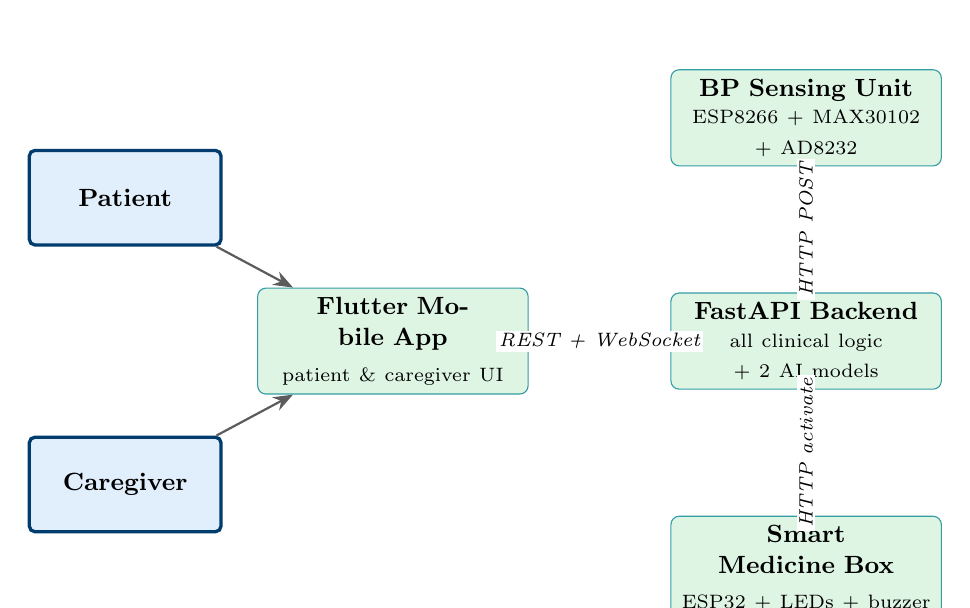
\begin{tikzpicture}[
  actorb/.style={rectangle, rounded corners=2pt, draw=primaryblue, very thick,
                 fill=nodeblue, text width=2.2cm, align=center, minimum height=1.2cm, font=\small\bfseries},
  sys/.style={rectangle, rounded corners=3pt, draw=accentteal!80, fill=nodegreen,
              text width=3.2cm, align=center, minimum height=1.1cm, font=\small}]
  \node[actorb] (pat) {Patient};
  \node[actorb, below=2.4cm of pat] (car) {Caregiver};

  \node[sys] at ($(pat)!0.5!(car)+(3.4,0)$) (app) {\textbf{Flutter Mobile App}\\[2pt]\scriptsize patient \& caregiver UI};
  \node[sys, right=1.8cm of app] (be) {\textbf{FastAPI Backend}\\[2pt]\scriptsize all clinical logic\\+ 2 AI models};
  \node[sys, above=1.6cm of be] (bp) {\textbf{BP Sensing Unit}\\[2pt]\scriptsize ESP8266 + MAX30102\\+ AD8232};
  \node[sys, below=1.6cm of be] (box) {\textbf{Smart Medicine Box}\\[2pt]\scriptsize ESP32 + LEDs + buzzer};

  \draw[flow] (pat) -- (app);
  \draw[flow] (car) -- (app);
  \draw[{Stealth[length=2mm]}-{Stealth[length=2mm]}, thick, draw=darkgray!80] (app) -- node[lbl]{REST + WebSocket} (be);
  \draw[flow] (bp) -- node[lbl,rotate=90]{HTTP POST} (be);
  \draw[flow] (be) -- node[lbl,rotate=90]{HTTP activate} (box);
\end{tikzpicture}
}%
\caption{System context: two human actors, one shared mobile app, one backend
that owns every clinical decision, and two purpose-built IoT devices.}
\label{fig:context}
\end{figure}

The system was built as a full \emph{vertical slice} rather than a collection
of independent components: custom sensor hardware that captures a real
physiological signal, a trained model that turns that raw signal into a
clinical number, a backend that owns every safety-relevant decision so the
hardware itself never has to be trusted with one, and a mobile app that
presents the same underlying data appropriately to a patient and to a
caregiver from shared code. Building all four layers together, integrated and
actually running against each other rather than validated in isolation, is
what distinguishes this project's engineering effort from a single training
notebook or a single mobile-app prototype --- and it is also why the honest
gaps documented throughout this report (Chapter~\ref{sec:results},
Section~\ref{sec:screenshots}, and the reliability notes in
Chapter~\ref{sec:conclusion}) are named plainly rather than hidden: a system
this size, built by a graduation-project team, will have real rough edges, and
stating them precisely is more useful to a reader than pretending otherwise.

\subsection{Project Objectives}

The objectives below are stated as they are evidenced by what was actually
built and measured, not as aspirations:

\begin{itemize}[leftmargin=1.4em]
  \item Deliver cuffless blood-pressure estimation accurate enough to be
  clinically useful, measured against the AAMI and BHS standards --- currently
  achieved for diastolic pressure, not yet for systolic.
  \item Make blood-pressure measurement a guided, low-friction routine through
  scheduled reminders and a step-by-step in-app flow, rather than a manual,
  easy-to-skip task.
  \item Give caregivers near-real-time visibility into a linked patient's
  vitals, medication adherence, and risk alerts without the patient having to
  actively share anything after the initial link.
  \item Improve real-world blood-pressure accuracy per patient via a
  calibration mechanism that learns from occasional reference cuff readings.
  \item Reduce missed medication doses via scheduled reminders plus an optional
  physical LED/buzzer indicator on a smart medicine box.
  \item Provide a symptom-triage capability that can stand alone or be
  triggered directly from a concerning blood-pressure reading, with a
  safety-first rule engine that can escalate urgency independently of the ML
  prediction and never let the model suppress a red flag.
  \item Support Arabic and English as first-class, parallel experiences rather
  than a translated afterthought.
\end{itemize}

\section{Contribution to Scientific Discovery}

The project's technical contribution centers on two applied machine-learning
efforts, and both are documented here with their real, measured results rather
than a single flattering headline number chosen after the fact:

\begin{itemize}[leftmargin=1.4em]
  \item A \textbf{cuffless blood-pressure estimation pipeline} that trains and
  fairly compares ten different models --- six classical regressors and four
  deep-learning architectures --- on an identical, record-level split of a
  MIMIC-derived dataset of over 650{,}000 signal windows. The headline result
  runs directly against the intuitive expectation going into the project: the
  team's own purpose-built architecture, which combines a temporal
  convolutional network encoder, a bidirectional LSTM, and multi-head
  self-attention specifically to capture rich temporal structure, did
  \emph{not} outperform a considerably simpler plain one-dimensional
  convolutional network trained on the same data with the same features. That
  result is reported as measured, not explained away, and Chapter~\ref{sec:results}
  discusses why it plausibly happened.
  \item A \textbf{structured symptom-triage model} that deliberately replaces an
  earlier free-text/TF-IDF representation with a severity-, duration-, age-,
  and vitals-aware structured feature vector, precisely because a bag-of-words
  representation has no way to encode ``a mild headache for two days'' as
  different from ``a severe headache for two weeks.'' Evaluating this new
  representation against simpler baselines trained on the identical data
  surfaces a second counter-intuitive finding: a plain Logistic Regression
  baseline scores higher than the LightGBM model that was actually chosen for
  production. Encountering the same pattern independently in two unrelated
  subsystems is itself a transferable finding, not a coincidence to be
  explained away in either case.
  \item A \textbf{per-patient calibration subsystem} for the blood-pressure
  model that adapts a population-trained model to one specific individual
  without ever retraining the model itself --- starting from a
  noise-resistant median offset and automatically upgrading to a full linear
  fit once enough reference readings accumulate, with a separate scheduled job
  that watches for the fit drifting out of date against the patient's own
  history. This is evaluated here against its own honestly inconclusive
  simulation result (Section~\ref{sec:calibration}) rather than assumed to
  work simply because the mechanism is well-designed.
  \item \textbf{Methodological discipline that eliminates a whole class of bug
  by construction.} For both AI subsystems, the exact same
  preprocessing/feature-engineering code that produced the training data is
  imported directly by the production inference path, rather than
  reimplemented a second time. This guarantees that what the model sees in
  production is mathematically identical to what it saw during training --- a
  guarantee that is usually only aspirational in applied ML systems, where
  training and inference code drift apart silently over time as one side is
  updated and the other is not.
\end{itemize}


%==============================================================================
\chapter{Related Work}
%==============================================================================

\section{Cuffless Blood Pressure Estimation}

Cuffless blood-pressure estimation from photoplethysmography (PPG) and
electrocardiography (ECG) signals is a well-known hard problem in biomedical
signal processing, and the physiological basis for attempting it at all is
real: the \emph{pulse transit time} (PTT) --- the delay between the electrical
activation of the heart, seen as the ECG R-peak, and the arrival of the
resulting pressure wave at a peripheral site, seen as the PPG peak --- is
inversely related to arterial pressure, because a stiffer, more pressurized
artery propagates a pulse wave faster than a more compliant one. Early
cuffless approaches, such as Kachuee et al.~\cite{kachuee2015}, built explicit
regression models directly on PTT and a small set of other hand-crafted
waveform features. The persistent difficulty with this line of work is that
the relationship between these features and true blood pressure is nonlinear,
patient-dependent, and confounded by vascular tone, age, and the specific
measurement site, which caps the accuracy any purely feature-based model can
reach across a diverse population --- a ceiling this project's own results
reproduce (Section~\ref{sec:bpfeatures} and Chapter~\ref{sec:results}).

More recent work has shifted toward deep learning applied directly to the raw
waveform, letting the model learn morphological features beyond hand-crafted
PTT rather than depending entirely on it~\cite{ppgbp2021,ppgdl2021}. A
recurring caveat across essentially all of this literature is dataset
provenance: the most common public benchmark for this problem is derived from
the MIMIC critical-care database~\cite{mimic3}, whose arterial-line reference
pressures come from ICU patients on invasive monitoring, not from ambulatory
or otherwise healthy subjects. A model trained on that distribution does not
automatically generalize to the resting, largely healthy or moderately
hypertensive home-use population that a wearable consumer product actually
targets --- a limitation this project inherits directly, and states plainly
rather than glossing over (Chapter~\ref{sec:results}).

This project's dataset handling and general preprocessing pipeline --- bandpass
filtering, resampling to a common rate, and peak-based reference-label
extraction from the arterial-line waveform itself --- follow the same broad
approach already established across the MIMIC-based cuffless-BP literature,
rather than introducing a novel signal-processing method of its own. The
project's genuine contribution sits one level up from preprocessing: a
controlled, ten-model comparison run on an identical record-level split so
that every model is judged on exactly the same evidence; a fault-tolerant,
resumable training pipeline built to survive a shared, quota-limited GPU
environment; and a per-patient calibration layer built on top of the
population-trained model, addressing the generalization gap above not by
collecting more diverse training data (which was not available) but by
adapting the deployed model to each individual patient after the fact.

\section{Rule-Based Clinical Decision Support}

On the symptom-checker side, rule-based clinical decision support --- red-flag
detection and escalation-only urgency rules layered on top of a statistical
classifier --- is an established, deliberately conservative design pattern in
clinical software. Its value is specific and well understood: it lets a
statistical model's errors be caught by a simpler, fully auditable safety net,
one that a clinician can read, reason about, and sign off on line by line in a
way that a gradient-boosted decision ensemble's internal weights cannot be. The
project's own rule engine (Section~\ref{sec:ruleengine}) follows this
established principle rather than inventing a new safety paradigm, and is
deliberately implemented as pure, independently testable functions kept
entirely separate from the ML classifier's code path --- so that the safety
layer's behavior is fully determined by its documented inputs and never by
anything the model happens to have learned.

The specific modeling choices also sit within the current mainstream of
applied machine learning: a gradient-boosted tree model
(LightGBM~\cite{lightgbm}) for the structured symptom classifier, and a direct
comparison against a modern attention-based architecture~\cite{attention} on
the blood-pressure side. What is less common is reporting, without spin, that
the simpler alternative won in both comparisons. That finding is a genuinely
useful, honestly-measured data point for the broader and still-open question
of when additional architectural sophistication is actually justified by the
data available, rather than assumed to help by default.

\section{Internal Comparative History}

The project's own internal history is itself a form of comparative evidence,
and is worth reading as a timeline rather than a single decision. Two earlier,
larger, less-regularized blood-pressure model attempts --- referred to
internally in the training notebook as ``v4'' and ``v10'' --- are documented
directly alongside the final results: v4 used no L2 regularization at all and
produced an 86\% train/validation MAE gap, a textbook case of severe
overfitting; v10 attempted to fix class imbalance by discarding real training
windows down to an equal count per class, which threw away most of the usable
dataset and made the model measurably worse overall rather than better. Both
failures directly and traceably shaped the final configuration used in this
project: inverse-frequency sample weighting in place of downsampling, so no
real data is thrown away, and a lighter, carefully re-tuned regularization
scheme that closes most of the overfitting gap without under-fitting the
model. Retaining this lineage of failed and refined attempts in the
documentation, rather than presenting only the final configuration as if it
were obvious from the start, is a more honest and more useful account of the
actual engineering process than a single final number ever could be.


%==============================================================================
\chapter{Software Description}
%==============================================================================

\section{Software Architecture}
\label{sec:arch}

Health Mate is composed of four cooperating parts: a Flutter mobile client
serving both patient and caregiver roles, a FastAPI backend that owns all
business logic and state, two purpose-built AI models, and two independent IoT
devices. A managed WebRTC voice/video calling layer connects patients and
caregivers directly. Figure~\ref{fig:sysarch} shows the full architecture and
the protocols each edge uses.

\begin{figure}[H]
\centering
\resizebox{\linewidth}{!}{%
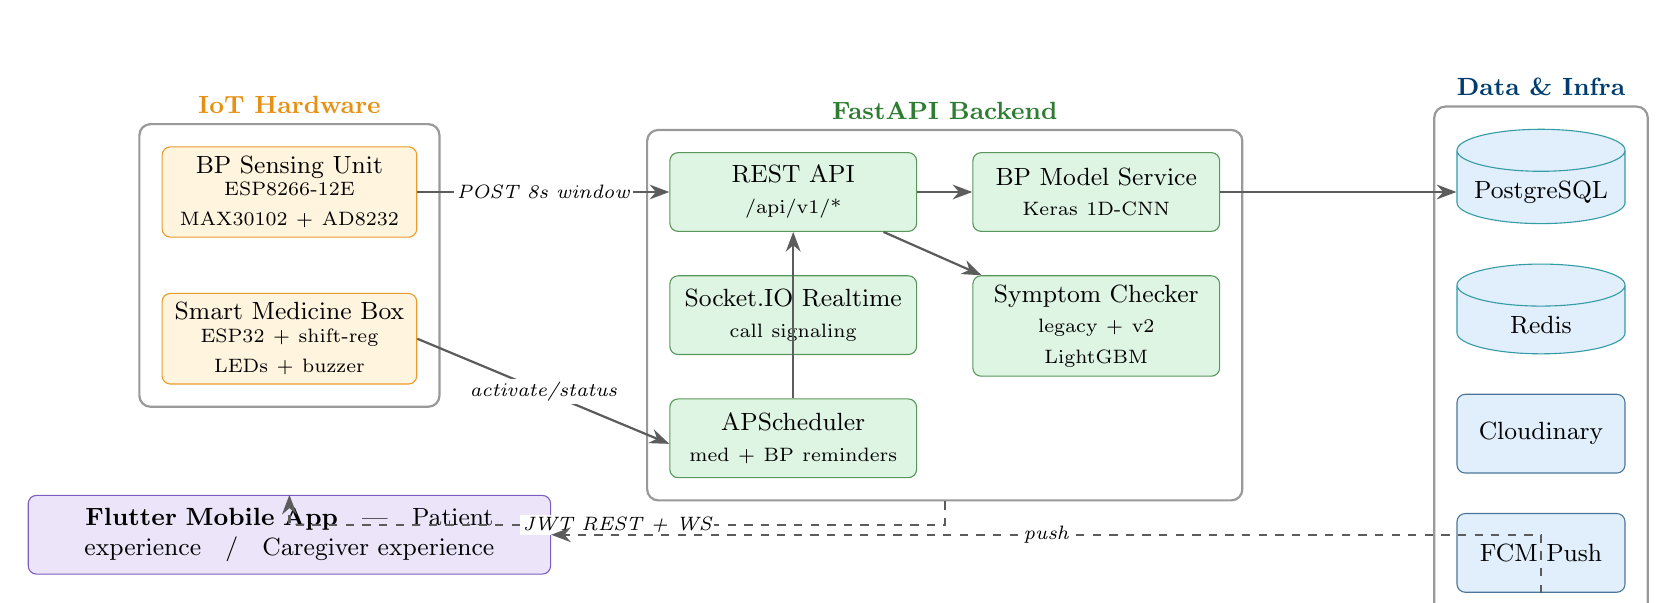
\begin{tikzpicture}[font=\footnotesize, node distance=0.7cm]
% ---- Hardware group ----
\node[abox, text width=3.0cm] (bpdev) {BP Sensing Unit\\\scriptsize ESP8266-12E\\MAX30102 + AD8232};
\node[abox, text width=3.0cm, below=0.7cm of bpdev] (box) {Smart Medicine Box\\\scriptsize ESP32 + shift-reg\\LEDs + buzzer};
\begin{scope}[on background layer]
\node[layer, fit=(bpdev)(box), label={[font=\small\bfseries\color{softamber}]above:IoT Hardware}] (hw) {};
\end{scope}

% ---- Backend group ----
\node[gbox, right=3.2cm of bpdev, text width=2.9cm] (api) {REST API\\\scriptsize /api/v1/*};
\node[gbox, below=0.55cm of api, text width=2.9cm] (ws) {Socket.IO Realtime\\\scriptsize call signaling};
\node[gbox, below=0.55cm of ws, text width=2.9cm] (sched) {APScheduler\\\scriptsize med + BP reminders};
\node[gbox, right=0.7cm of api, text width=2.9cm] (bpmodel) {BP Model Service\\\scriptsize Keras 1D-CNN};
\node[gbox, below=0.55cm of bpmodel, text width=2.9cm] (sym) {Symptom Checker\\\scriptsize legacy + v2 LightGBM};
\begin{scope}[on background layer]
\node[layer, fit=(api)(ws)(sched)(bpmodel)(sym),
      label={[font=\small\bfseries\color{softgreen}]above:FastAPI Backend}] (bemid) {};
\end{scope}

% ---- Data group ----
\node[db, right=3.0cm of bpmodel] (pg) {PostgreSQL};
\node[db, below=0.5cm of pg] (redis) {Redis};
\node[box, below=0.5cm of redis, text width=1.9cm] (cloud) {Cloudinary};
\node[box, below=0.5cm of cloud, text width=1.9cm] (fcm) {FCM Push};
\begin{scope}[on background layer]
\node[layer, fit=(pg)(redis)(cloud)(fcm),
      label={[font=\small\bfseries\color{primaryblue}]above:Data \& Infra}] (data) {};
\end{scope}

% ---- Mobile ----
\node[pbox, below=1.4cm of box, text width=6.4cm] (mobile)
  {\textbf{Flutter Mobile App} \; --- \; Patient experience \; / \; Caregiver experience};

% ---- Edges ----
\draw[flow] (bpdev.east) -- node[lbl]{POST 8s window} (api.west);
\draw[flow] (box.east) -- node[lbl]{activate/status} ([yshift=-2pt]sched.west);
\draw[flow] (api) -- (bpmodel);
\draw[flow] (api) -- (sym);
\draw[flow] (bpmodel.east) -- (pg.west);
\draw[flow] (sched) -- (api);
\draw[flow, dashed] (bemid.south) -- ++(0,-0.3) -| node[lbl,pos=0.25]{JWT REST + WS} (mobile.north);
\draw[flow, dashed] (fcm.south) |- node[lbl,pos=0.75]{push} (mobile.east);
\end{tikzpicture}
}%
\caption{Health Mate system architecture. The hardware never makes clinical
decisions --- every safety-relevant step runs in the backend.}
\label{fig:sysarch}
\end{figure}

The system is deliberately split so that \textbf{the hardware never makes
clinical decisions}. Both the blood-pressure unit and the smart box are data
collectors / actuators only: the ESP8266 firmware buffers 800 raw PPG/ECG
samples, checks finger/lead gating, and posts the window to the backend; it
contains no model, no calibration, and no risk logic. Every clinically
meaningful step --- signal validation, model inference, calibration, drift
detection, risk classification, and alerting --- runs in the backend. This is a
verifiable property of the code, not merely stated intent.

\subsection{Two Architectural Styles, Side by Side}

The backend mixes two architectural styles, and it is worth being explicit
about that rather than pretending it is uniform:

\begin{itemize}[leftmargin=1.4em]
  \item \textbf{Service-layer style} (most of the system). Authentication,
  medications, vitals, notifications, contacts, calls, IoT device management,
  and the BP reminder/calibration/drift logic all follow a straightforward
  pattern: FastAPI routers call flat service modules, which talk directly to
  SQLAlchemy models. There is no repository abstraction here --- this is simple,
  easy to trace, and dominant across the codebase.
  \item \textbf{Clean/hexagonal architecture} (symptom checker v2). The newer
  symptom-checker implementation is structured as a deliberate, documented
  refactor with a genuine dependency-inversion boundary
  (Figure~\ref{fig:cleanarch}). Use cases depend on domain interfaces, and a
  single dependency-injection module decides which concrete infrastructure
  implementation satisfies each interface.
\end{itemize}

\begin{figure}[H]
\centering
\resizebox{\linewidth}{!}{%
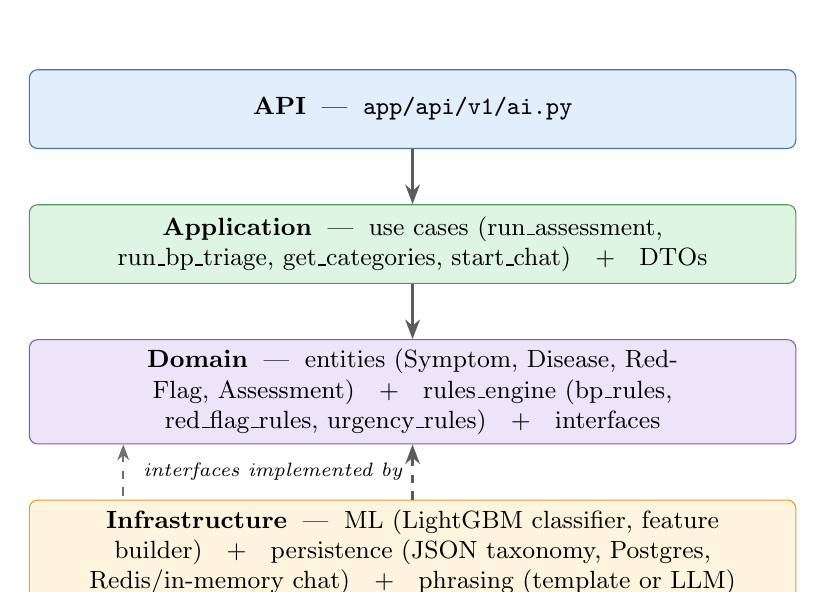
\begin{tikzpicture}[font=\footnotesize, node distance=0.55cm]
\node[box, text width=9.5cm] (apilayer) {\textbf{API} \;---\; \texttt{app/api/v1/ai.py}};
\node[gbox, below=0.7cm of apilayer, text width=9.5cm] (applayer)
  {\textbf{Application} \;---\; use cases (run\_assessment, run\_bp\_triage,
   get\_categories, start\_chat) \; + \; DTOs};
\node[pbox, below=0.7cm of applayer, text width=9.5cm] (domlayer)
  {\textbf{Domain} \;---\; entities (Symptom, Disease, RedFlag, Assessment) \; +
   \; rules\_engine (bp\_rules, red\_flag\_rules, urgency\_rules) \; + \; interfaces};
\node[abox, below=0.7cm of domlayer, text width=9.5cm] (infralayer)
  {\textbf{Infrastructure} \;---\; ML (LightGBM classifier, feature builder) \;
   + \; persistence (JSON taxonomy, Postgres, Redis/in-memory chat) \; + \;
   phrasing (template or LLM)};
\draw[flow] (apilayer) -- (applayer);
\draw[flow] (applayer) -- (domlayer);
\draw[{Stealth[length=2mm]}-, thick, dashed, draw=darkgray!70]
   (domlayer.south west) ++(1.2,0) -- ++(0,-0.7)
   node[lbl, pos=0.5, xshift=1.9cm]{interfaces implemented by};
\draw[flow, dashed] (infralayer.north) -- (domlayer.south);
\end{tikzpicture}
}%
\caption{Clean-architecture layering used for the symptom checker v2: the only
subsystem restructured this way. Dependencies point inward; infrastructure
implements domain interfaces, wired in one dependency-injection module.}
\label{fig:cleanarch}
\end{figure}

This layered structure exists \emph{only} for the symptom checker. An older,
simpler implementation is still loaded at application startup alongside the v2
path; the two coexist, gated by a backend setting. The point here is
architectural: this is the one part of the backend deliberately restructured,
and the rest has intentionally been left in its simpler, already-working form.

\subsection{Cross-Cutting Backend Pieces}

\begin{itemize}[leftmargin=1.4em]
  \item \textbf{Configuration} --- a single Pydantic \texttt{Settings} object
  sourced from environment variables, covering the database, Redis, JWT, IoT
  mode, AI model paths, Cloudinary, Firebase, WebRTC STUN/TURN servers, and
  CORS. No hardcoded configuration values live in application code.
  \item \textbf{Security} --- JWT issuance and verification (access + refresh
  tokens), and bcrypt password hashing.
  \item \textbf{Scheduler} --- APScheduler background jobs. Medication reminders
  are cron-style jobs; when one fires, the backend looks up matching
  medications, optionally activates smart-box drawers, and sends a
  notification. BP reminders use the same mechanism.
  \item \textbf{Realtime layer} --- a \texttt{python-socketio} async server
  mounted onto the FastAPI app, authenticated with the same JWT, used
  specifically for WebRTC call signaling.
  \item \textbf{Firebase Cloud Messaging} --- push notifications (medication
  alarms, BP reminders, critical-vitals alerts), separate from the Socket.IO
  channel.
  \item \textbf{PostgreSQL + Alembic} --- the system of record, with a migration
  history that traces the project's real build-out.
\end{itemize}

\section{Tools and Technologies Used}

The technology choices below were made for concrete, stated reasons rather than
by default (Table~\ref{tab:tools}).

\begin{table}[H]
\centering
\caption{Technology stack and rationale.}
\label{tab:tools}
\small
\begin{tabularx}{\linewidth}{@{}>{\raggedright\arraybackslash}p{2.4cm}>{\raggedright\arraybackslash}p{4.7cm}Y@{}}
\toprule
\textbf{Layer} & \textbf{Technology} & \textbf{Why chosen} \\
\midrule
Mobile client & Flutter, Riverpod, Dio + Retrofit, Hive,
flutter\_secure\_storage, easy\_localization &
Cross-platform single codebase; Riverpod family providers let one set of
screens serve both patient and caregiver views; Hive gives offline-first
access to recent vitals \\
Backend & FastAPI (async), SQLAlchemy (async, asyncpg), Alembic, APScheduler,
python-socketio &
Non-blocking I/O suited to real-time telemetry; APScheduler drives reminders;
Socket.IO handles WebRTC call signaling \\
Data & PostgreSQL 15, Redis &
Postgres as the relational system of record; Redis for app-level caching and
chat-session state \\
BP model & TensorFlow/Keras, scikit-learn, XGBoost, LightGBM, CatBoost &
A deliberately broad model comparison rather than committing to one
architecture upfront \\
Symptom checker & LightGBM (v2, structured), scikit-learn (v1, TF-IDF, legacy) &
LightGBM for the new structured feature set; the older pipeline retained, not
deleted \\
Notifications & Firebase Cloud Messaging, flutter\_local\_notifications &
Cloud push for reliability, local scheduling for offline reminder delivery \\
Media & Cloudinary & Profile and medication/adherence photo uploads \\
Calling & flutter\_webrtc, Socket.IO signaling &
Direct patient/caregiver audio/video without a third-party calling SDK \\
Deployment & Docker Compose & Single-host development/demo deployment \\
Firmware & Arduino / C++ (ESP8266, ESP32) &
Low-cost, WiFi-capable microcontrollers matched to the model's 100\,Hz input
contract \\
\bottomrule
\end{tabularx}
\end{table}

\section{Software Functionalities}

The features below are the ones that actually exist in the codebase; the
use-case catalogue in Table~\ref{tab:usecases} records their implementation
evidence, and the use-case diagram in Figure~\ref{fig:usecase} groups them by
actor.

\begin{itemize}[leftmargin=1.4em]
  \item \textbf{Authentication} --- email/password and Firebase (social)
  sign-up and login, JWT access + refresh tokens, role selection at
  registration.
  \item \textbf{Patient--caregiver linking} --- link by user ID (with a QR-code
  UI on top), multiple caregivers per patient, one designated primary
  caregiver, and unlinking.
  \item \textbf{Guided blood-pressure measurement} --- an 8-second sensor
  capture walked through step by step, feeding the backend's model + calibration
  pipeline, with results withheld from the patient as a raw number until
  calibration is trustworthy.
  \item \textbf{Per-patient calibration and drift detection} --- a two-tier fit
  (robust median offset below 8 samples, full linear regression above), with a
  scheduled job flagging sustained drift or staleness.
  \item \textbf{BP measurement reminders} --- up to three daily reminder times
  derived from one patient-chosen start time.
  \item \textbf{Medication management} --- catalog with dosage/schedule,
  optional smart-box drawer assignment, scheduled alarms (push + local
  notification + optional LED/buzzer), adherence logging with optional photo
  proof.
  \item \textbf{Structured symptom triage} --- a severity/duration/age/
  vitals-aware assessment wizard backed by a rule engine, plus a direct handoff
  from a concerning BP reading into the same triage flow.
  \item \textbf{Emergency alerting} --- automatic caregiver push on
  high/critical BP or red-flag symptoms, rate-limited per risk tier.
  \item \textbf{Medical contacts} --- doctor/clinic/pharmacy/emergency/family
  contact list per patient, with the caregiver auto-added as a family contact
  on linking.
  \item \textbf{Audio/video calling} --- WebRTC calls between a patient and a
  linked caregiver, with dedicated incoming-call and emergency-call screens.
  \item \textbf{Notifications inbox} --- in-app list of all past notifications,
  read/unread state.
  \item \textbf{Localization} --- full English/Arabic parity with RTL support.
  \item \textbf{Offline support} --- cached last-known BP reading and history
  (Hive-backed); reminders continue to fire locally without connectivity.
\end{itemize}

\clearpage
\section{Functional Requirements}

The functional requirements in Table~\ref{tab:functional-reqs} summarize what
the implemented system must do from a user and system-behavior perspective.

\begingroup
\small
\setlength{\LTpre}{0.3em}
\setlength{\LTpost}{0.3em}
\begin{longtable}{@{}>{\raggedright\arraybackslash}p{4.4cm}>{\raggedright\arraybackslash}p{10.0cm}@{}}
\caption{Functional requirements.}\label{tab:functional-reqs}\\
\toprule
\textbf{Requirement} & \textbf{Implemented behavior} \\
\midrule
\endfirsthead
\multicolumn{2}{c}{\small\itshape Table~\ref{tab:functional-reqs} continued}\\
\toprule
\textbf{Requirement} & \textbf{Implemented behavior} \\
\midrule
\endhead
\bottomrule
\endfoot
Account registration and login & Patients and caregivers can create accounts, sign in, refresh sessions, and use Firebase/social authentication. \\
Role-based experience & The mobile application opens patient or caregiver workflows according to the saved account role. \\
Patient-caregiver linking & Patients and caregivers can link, unlink, and maintain one active primary caregiver for a patient. \\
Guided BP measurement & The BP device sends an 800-sample PPG/ECG window; the backend stores a result or a clear rejection reason. \\
Calibration and cuff confirmation & The backend asks for cuff confirmation when calibration is missing, weak, or due, then stores calibration samples. \\
Vitals history and monitoring & Patients and linked caregivers can view recent readings, history, and statistics. \\
BP reminders & Patients can schedule daily blood-pressure reminders from a selected start time. \\
Medication management & Patients can add, edit, delete, schedule, and assign medications to smart-box drawers. \\
Medication adherence & Patients can confirm medication intake, with optional image proof. \\
Smart-box activation & The backend or mobile app can activate drawer LEDs and buzzer when the smart box is reachable. \\
Symptom assessment & The app collects structured symptoms, severity, duration, age group, known conditions, and vitals, then returns urgency and action guidance. \\
Emergency notifications & Caregivers receive alerts for critical BP or high-risk symptom assessments, with cooldown protection. \\
Medical contacts & Patients can manage doctor, clinic, pharmacy, emergency, and family contacts. \\
Audio/video calling & Linked patients and caregivers can start, accept, reject, and end WebRTC calls. \\
Notification inbox & Users can list, read, mark, and delete notifications. \\
Localization & The mobile app supports English and Arabic, including RTL display for Arabic. \\
\end{longtable}
\endgroup

\clearpage
\section{Non-Functional Requirements}

The non-functional requirements in Table~\ref{tab:nonfunctional-reqs} describe
the quality constraints that shape the implementation.

\begingroup
\small
\setlength{\LTpre}{0.3em}
\setlength{\LTpost}{0.3em}
\begin{longtable}{@{}>{\raggedright\arraybackslash}p{4.4cm}>{\raggedright\arraybackslash}p{10.0cm}@{}}
\caption{Non-functional requirements.}\label{tab:nonfunctional-reqs}\\
\toprule
\textbf{Quality attribute} & \textbf{Implementation approach} \\
\midrule
\endfirsthead
\multicolumn{2}{c}{\small\itshape Table~\ref{tab:nonfunctional-reqs} continued}\\
\toprule
\textbf{Quality attribute} & \textbf{Implementation approach} \\
\midrule
\endhead
\bottomrule
\endfoot
Safety & Hardware devices collect signals or actuate alarms only; clinical decisions run in the backend. \\
Security & Human endpoints use JWT authentication, passwords are hashed, and BP hardware endpoints use device credentials. \\
Privacy & Health records, contacts, calls, notifications, and calibration data are scoped to the owning patient and authorized caregivers. \\
Reliability & Model-loading failures, poor signals, unreachable devices, and notification failures degrade gracefully. \\
Data integrity & PostgreSQL foreign keys, enums, constraints, and the primary-caregiver unique index protect the data model. \\
Maintainability & The project separates Flutter UI/data layers, FastAPI routers/services/models, migrations, and symptom-checker use cases. \\
Scalability & Async FastAPI/SQLAlchemy, PostgreSQL, and Redis support non-blocking API, persistence, and cache/session state. \\
Usability & Guided mobile flows reduce user mistakes during BP measurement, medication setup, symptom triage, and caregiver monitoring. \\
Localization & English and Arabic interfaces are supported, including RTL presentation for Arabic. \\
Portability & Flutter supports multi-platform mobile development, and Docker Compose provides repeatable backend deployment. \\
Auditability & Security and compliance events are stored in audit logs where available. \\
Offline tolerance & Recent vitals/history are cached and local reminder behavior can continue without connectivity. \\
\end{longtable}
\endgroup

\begin{table}[H]
\centering
\caption{Professional use-case catalogue for the implemented Health Mate system.}
\label{tab:usecases}
\small
\begin{tabularx}{\linewidth}{@{}>{\raggedright\arraybackslash}p{2.9cm}>{\raggedright\arraybackslash}p{3.8cm}Y@{}}
\toprule
\textbf{Primary actor} & \textbf{Use case} & \textbf{Implementation evidence and outcome} \\
\midrule
Patient & Register / sign in & FastAPI auth endpoints issue JWT access/refresh tokens; Flutter stores credentials securely and gates patient/caregiver navigation. \\
Patient, caregiver & Link / unlink accounts & \texttt{patient\_caregiver\_links} stores active patient-caregiver relationships, with one active primary caregiver per patient. \\
Patient & Take guided BP measurement & The BP device submits an 800-sample PPG/ECG window; the backend runs inference, calibration, status handling, and persistence. \\
Patient & Confirm cuff reading & Cuff confirmation completes pending readings and appends calibration samples for future per-patient correction. \\
Patient, caregiver & View vitals history & Vitals history and stats endpoints power patient charts and caregiver monitoring screens for linked patients. \\
Patient & Manage medications & Medication CRUD stores dosage, schedule, optional image, and optional smart-box drawer assignment. \\
Patient & Log adherence & Medication adherence records a taken timestamp and optional image proof rather than trusting the box as a physical retrieval sensor. \\
Patient & Run symptom assessment & The v2 structured assessment path combines selected symptoms, severity, duration, age group, vitals, red flags, and ML predictions. \\
Caregiver & Receive alerts & Notification services send caregiver alerts for critical BP and red-flag/high-urgency symptom assessments, with cooldown logic for BP tiers. \\
Patient, caregiver & Audio/video call & Call sessions track caller/callee, call type, status, offer/answer SDP, and lifecycle events used by the WebRTC UI. \\
Patient & Manage medical contacts & Contacts endpoints persist doctors, clinics, pharmacies, emergency contacts, and family contacts under the patient account. \\
\bottomrule
\end{tabularx}
\end{table}

\begin{figure}[H]
\centering
\resizebox{\linewidth}{!}{%
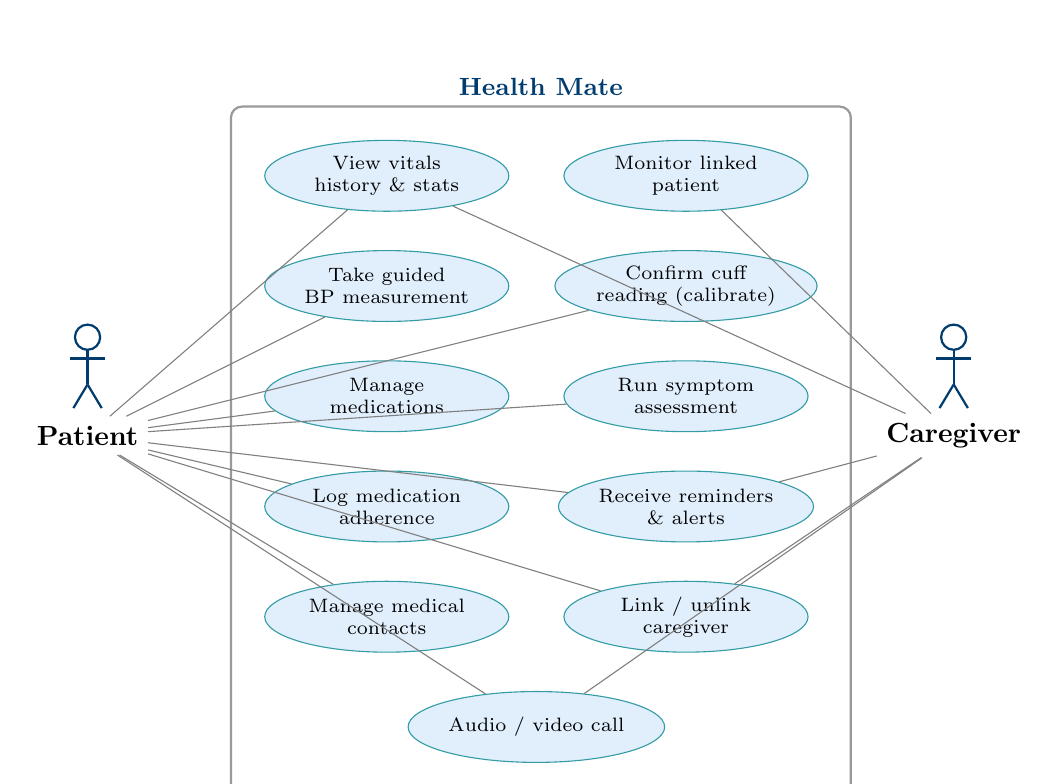
\begin{tikzpicture}[font=\footnotesize,
  stick/.pic={
    \draw[actor] (0,0.55) circle (0.16);
    \draw[actor] (0,0.39)--(0,-0.05);
    \draw[actor] (-0.22,0.28)--(0.22,0.28);
    \draw[actor] (0,-0.05)--(-0.18,-0.35);
    \draw[actor] (0,-0.05)--(0.18,-0.35);
  }]
% Actors (left = patient, right = caregiver)
\pic (patp) at (0,2) {stick};
\node[font=\bfseries] (pat) at (0,1.3) {Patient};
\pic (carp) at (11,2) {stick};
\node[font=\bfseries] (car) at (11,1.3) {Caregiver};

% Use cases -- columns centered at x=3.8 / x=7.6 (3.8cm apart) so that two
% 3.1cm-wide ellipses (half-width 1.55cm each) never touch (0.7cm clear gap).
\node[usecase] (uc1) at (3.8,3.2)  {Take guided\\BP measurement};
\node[usecase] (uc2) at (7.6,3.2)  {Confirm cuff\\reading (calibrate)};
\node[usecase] (uc3) at (3.8,1.8)  {Manage\\medications};
\node[usecase] (uc4) at (7.6,1.8)  {Run symptom\\assessment};
\node[usecase] (uc5) at (3.8,0.4)  {Log medication\\adherence};
\node[usecase] (uc6) at (7.6,0.4)  {Receive reminders\\\& alerts};
\node[usecase] (uc7) at (3.8,-1.0) {Manage medical\\contacts};
\node[usecase] (uc8) at (7.6,-1.0) {Link / unlink\\caregiver};
\node[usecase] (uc9) at (5.7,-2.4){Audio / video call};
\node[usecase] (uc10) at (3.8,4.6) {View vitals\\history \& stats};
\node[usecase] (uc11) at (7.6,4.6) {Monitor linked\\patient};

\begin{scope}[on background layer]
\node[layer, fit=(uc1)(uc2)(uc3)(uc4)(uc5)(uc6)(uc7)(uc8)(uc9)(uc10)(uc11),
      inner sep=12pt, label={[font=\small\bfseries\color{primaryblue}]above:Health Mate}] {};
\end{scope}

\foreach \u in {uc1,uc2,uc3,uc4,uc5,uc7,uc8,uc9,uc10,uc6}{\draw[-, gray] (pat) -- (\u);}
\foreach \u in {uc11,uc6,uc8,uc9,uc10}{\draw[-, gray] (car) -- (\u);}
\end{tikzpicture}
}%
\caption{Use-case diagram. Patients and caregivers share the calling, linking,
alerting, and monitoring use cases; measurement, calibration, medication, and
symptom assessment are patient-driven, while ``monitor linked patient'' is
caregiver-specific.}
\label{fig:usecase}
\end{figure}


%==============================================================================
\chapter{IoT Hardware Subsystems}
%==============================================================================

Health Mate has two entirely separate hardware subsystems --- a blood-pressure
sensing unit and a smart medicine box --- built on different microcontrollers,
different firmware, and different interaction models. They deliberately do not
share a microcontroller. Table~\ref{tab:hwcompare} summarizes the contrast.

\begin{table}[H]
\centering
\caption{The two IoT subsystems at a glance.}
\label{tab:hwcompare}
\small
\begin{tabularx}{\linewidth}{@{}>{\raggedright\arraybackslash}p{3.0cm}YY@{}}
\toprule
 & \textbf{BP sensing unit} & \textbf{Smart medicine box} \\
\midrule
MCU & ESP8266-12E NodeMCU & ESP32 \\
Sensors / actuators & MAX30102 (PPG, I2C), AD8232 (ECG, analog + lead-off pins) &
74HC595 shift register driving one LED per drawer, plus a buzzer --- no motors \\
Talks to backend how & Pushes data (POST /bp/submit, /bp/heartbeat) & Receives commands (POST /activate) \\
Authentication & Device ID + hashed token (real mechanism) & None --- plain HTTP, same-network trust \\
Actuation & None (pure sensor) & LEDs + buzzer only --- no physical dispensing \\
Failure mode & Retry with backoff; abort on auth rejection & Fail-soft: errors logged, alarm job continues \\
\bottomrule
\end{tabularx}
\end{table}

\section{Blood-Pressure Sensing Unit}

\subsection{Hardware}

\begin{itemize}[leftmargin=1.4em]
  \item \textbf{ESP8266-12E NodeMCU} --- WiFi microcontroller, no on-device model
  inference.
  \item \textbf{MAX30102} --- PPG sensor over I2C, configured with
  \texttt{sampleAverage = 1}, chosen specifically to produce raw, unaveraged
  100\,Hz output matching the trained model's expected input rate.
  \item \textbf{AD8232} --- single-lead ECG front-end, analog output on A0, with
  dedicated lead-off detection pins and a shutdown pin held high to keep the
  chip enabled.
\end{itemize}

The full breadboard wiring, the complete pin-connection tables for both sensors,
and the electrode-placement reference are shown in Figure~\ref{fig:wiring}. The
MAX30102 communicates over I2C (SDA on \texttt{D2}, SCL on \texttt{D1}); the
AD8232's analog output is read on \texttt{A0}, its shutdown pin is driven from
\texttt{D5}, and its two lead-off detection lines are on \texttt{D6}/\texttt{D7}.
A common ground between all three modules is required. Figure~\ref{fig:ecgplace}
shows the standard three-lead electrode placement on the body in more anatomical
detail.

\begin{figure}[H]
\centering
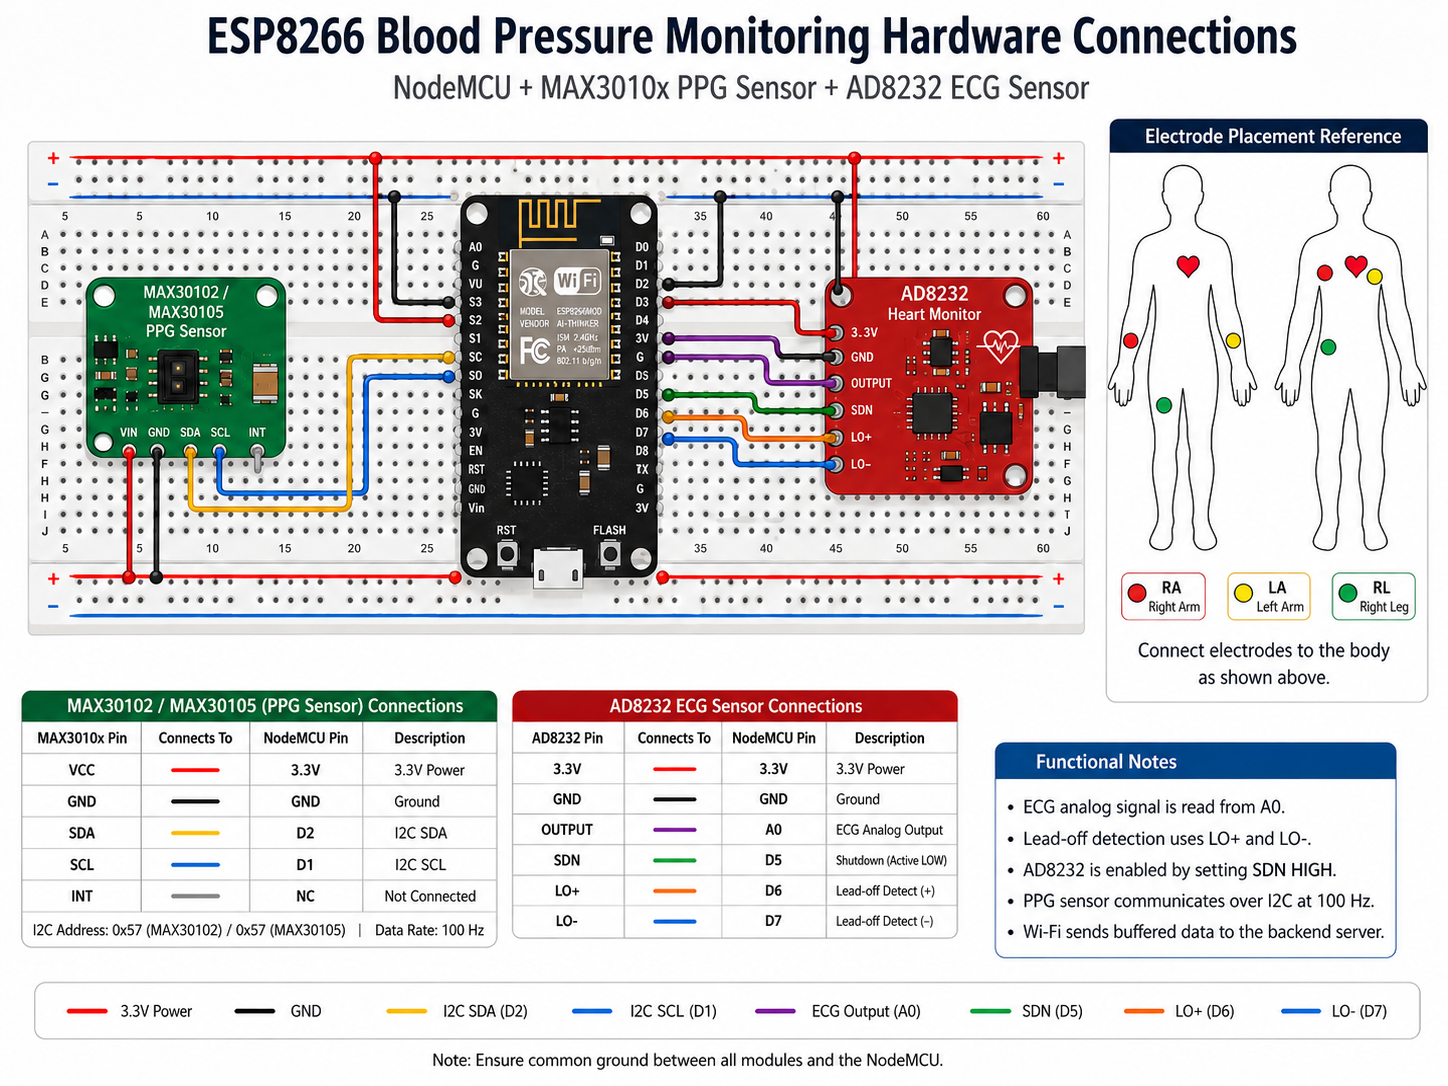
\includegraphics[width=0.98\linewidth]{bp_hardware_circuit.png}
\caption{Blood-pressure sensing unit --- complete hardware wiring (NodeMCU
ESP8266 + MAX30102 PPG + AD8232 ECG), with per-sensor pin tables, electrode
placement, and functional notes.}
\label{fig:wiring}
\end{figure}

\begin{figure}[H]
\centering
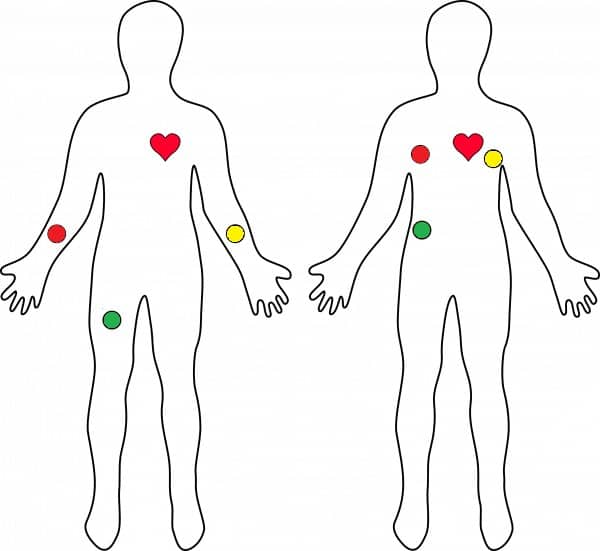
\includegraphics[width=0.42\linewidth]{ecg_lead_placement.jpg}
\caption{AD8232 three-lead (RA/LA/RL) electrode placement on the torso and
limbs, shown in two equivalent placement variants.}
\label{fig:ecgplace}
\end{figure}

\subsection{Firmware Behavior}

This is real, working firmware, not a wiring test. The behavior below is
confirmed directly in the source:

\begin{itemize}[leftmargin=1.4em]
  \item Samples both channels at a precise 100\,Hz, buffering exactly 800
  samples per channel --- an 8-second window matching the model's input
  contract.
  \item \textbf{Gates on signal presence} before accepting any sample: both ECG
  leads connected \emph{and} a finger detected on the PPG sensor (IR $>$ 50{,}000
  counts). If gating fails for 50 consecutive checks ($\sim$500\,ms), the
  in-progress buffer is discarded rather than silently accepting a bad window.
  \item Computes \textbf{on-device SpO2} (ratio-of-ratios) and \textbf{heart
  rate} (peak detection), included in the payload only when physiologically
  plausible --- an unusable value is omitted, not sent as a placeholder.
  \item \textbf{Uploads the completed window} via HTTP POST with device-ID and
  device-token headers and an exponential-backoff retry policy (up to 4
  attempts), except on a 401/403/422 response, treated as a permanent rejection
  and aborted immediately.
  \item \textbf{Sends a heartbeat} on a 10-second timer, or immediately (at most
  once per second) whenever the finger/lead state changes, so the backend's
  device flags reflect a mid-measurement disconnection within about a second.
\end{itemize}

\textbf{A real, unresolved gap:} the device token in the current firmware is a
hardcoded placeholder string, not a per-device provisioned secret. The
authentication \emph{mechanism} (hashed token compared server-side) is real and
correct, but the credential shipped in this firmware file is not
production-grade.

\section{Smart Medicine Box}

\subsection{Hardware --- an Explicit Correction}

The smart box is an ESP32 running its own tiny web server on port 80, a 74HC595
shift register driving up to 6 LEDs (one per drawer), and a buzzer.
\textbf{There is no motor, servo, solenoid, or physical locking/dispensing
mechanism anywhere in the firmware.} Concretely, the smart box \emph{indicates}
which drawer to open --- it does not open it. On receiving an activation payload
such as \texttt{\{"drawers": [3]\}}, it lights the corresponding LED(s) and runs
an intermittent buzzer alert; an empty list turns everything off. The patient
still physically opens the correct drawer once the LED points to it. Any
description of this as ``automatically dispensing'' overstates the hardware; it
is a guided-indicator system --- still a real and useful piece of assistive
hardware for an elderly or memory-impaired patient, but a materially simpler and
more reliable mechanism than a motorized dispenser.

The physical build and full wiring are shown in Figure~\ref{fig:boxwiring}: a
laser-cut wooden enclosure with six medication compartments and an acrylic
window, an ESP32 driving a 74HC595 shift register (data on \texttt{GPIO23},
clock on \texttt{GPIO18}, latch on \texttt{GPIO5}), the register's
\texttt{Q0}--\texttt{Q5} outputs lighting the six drawer LEDs through current-
limiting resistors, and an active buzzer on \texttt{GPIO4}.

\begin{figure}[H]
\centering
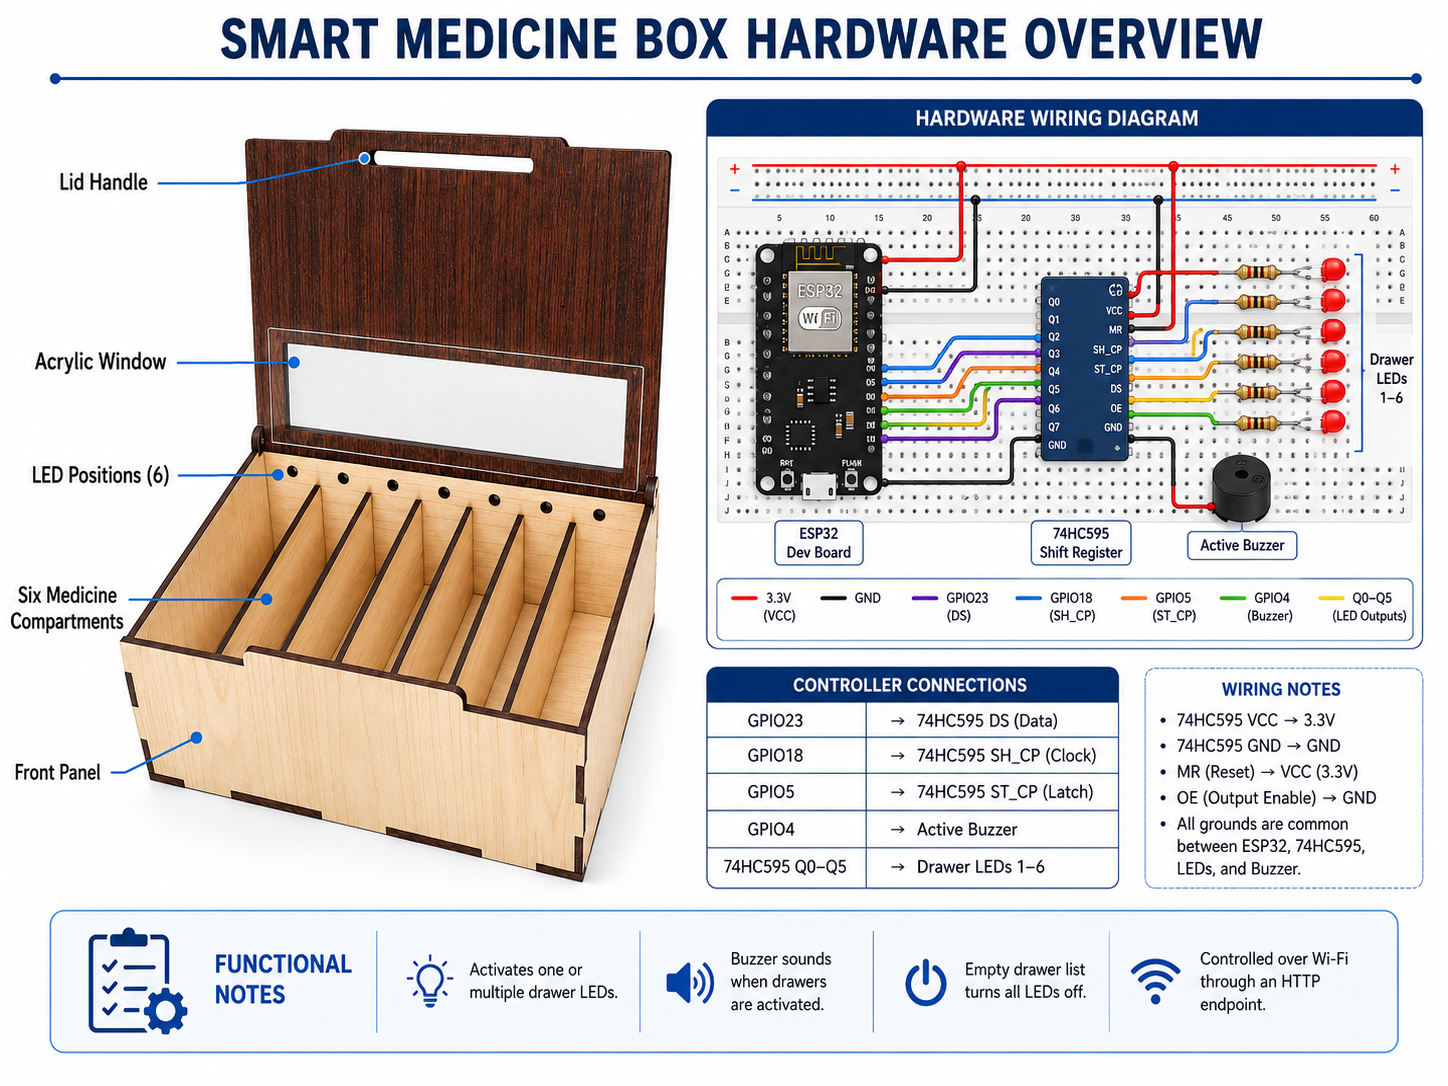
\includegraphics[width=0.98\linewidth]{smart_box_circuit.png}
\caption{Smart medicine box --- physical enclosure (six compartments, LED
positions, acrylic window) and complete hardware wiring (ESP32 + 74HC595 shift
register + six drawer LEDs + active buzzer), with the controller pin map and
functional notes.}
\label{fig:boxwiring}
\end{figure}

\subsection{Who Talks to It}

Two independent callers can activate the box:

\begin{enumerate}[leftmargin=1.6em]
  \item \textbf{The backend scheduler} --- when a medication alarm fires, it
  collects the drawers due at that time and calls activate(); the call is
  fail-soft, so an unreachable box never crashes the alarm job.
  \item \textbf{The Flutter app directly} --- it can make its own HTTP call
  straight to the ESP32's local IP, bypassing the backend, as long as the phone
  is on the same network as the box.
\end{enumerate}

\subsection{Reliability Characteristics}

\begin{itemize}[leftmargin=1.4em]
  \item \textbf{No acknowledgment of physical retrieval} --- because no sensor
  detects whether a drawer was opened, adherence is logged from the patient
  explicitly confirming ``taken'' in the app, not from any hardware signal.
  \item \textbf{Offline behavior} --- if the ESP32 is unreachable when an alarm
  fires, the LED/buzzer step is silently skipped, but the phone push/local
  notification for the same reminder is unaffected.
  \item \textbf{Multiple medications at the same time} are collected into one
  activation call, lighting multiple LEDs simultaneously.
\end{itemize}


%==============================================================================
\chapter{Database Design}
%==============================================================================

Health Mate's system of record is PostgreSQL 15, accessed through SQLAlchemy's
async ORM and versioned with Alembic. The schema comprises 21 model classes.
Figure~\ref{fig:er} shows the core entities and their relationships;
Table~\ref{tab:tables} lists every table.

\section{Entity-Relationship Diagram}

The ERD in Figure~\ref{fig:er} is the project-maintained diagram exported from
the implemented backend schema. Because the source is a wide diagram, it is
placed as one complete landscape page instead of being split into cropped
pieces. In print, this page should be printed in landscape orientation.

\clearpage
\begin{landscape}
\thispagestyle{empty}
\begin{figure}[p]
\centering
\vspace*{-0.4cm}
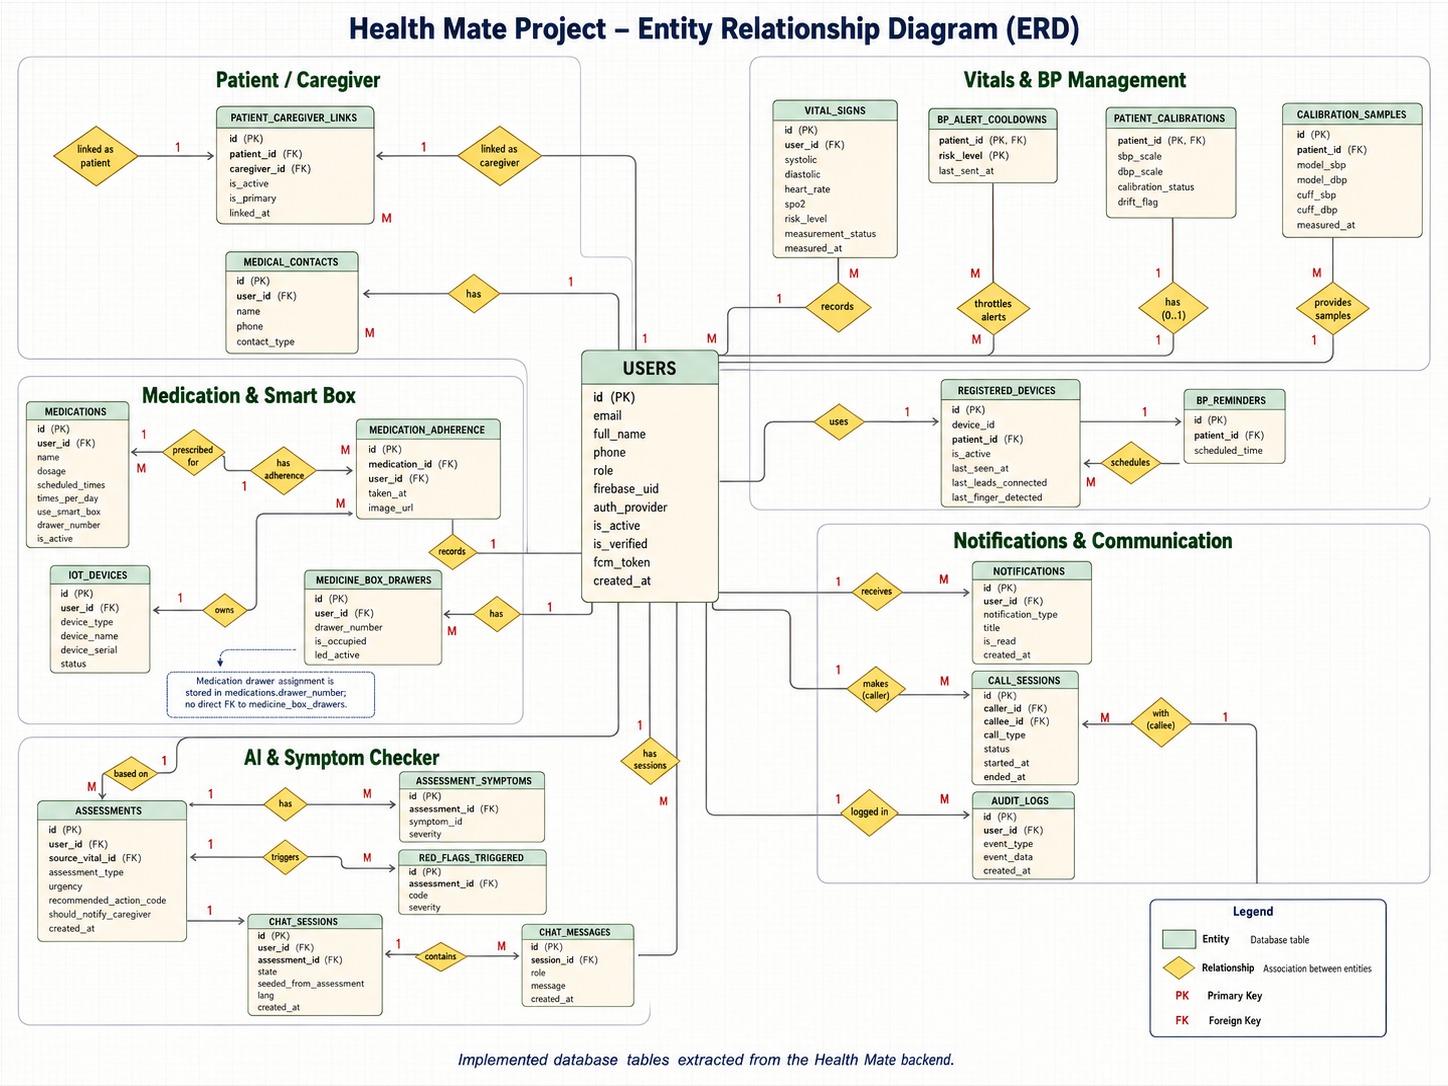
\includegraphics[width=0.98\linewidth,height=0.82\textheight,keepaspectratio]{Health_Mate_ERD_diagram.png}
\caption{Complete entity-relationship diagram for the implemented Health Mate
backend schema.}
\label{fig:er}
\end{figure}
\end{landscape}
\clearpage

\section{Tables at a Glance}

\begin{longtable}{@{}>{\raggedright\arraybackslash}p{3.4cm}>{\raggedright\arraybackslash}p{7.0cm}>{\raggedright\arraybackslash}p{4.3cm}@{}}
\caption{The 21 tables of the Health Mate schema.}\label{tab:tables}\\
\toprule
\textbf{Table} & \textbf{Purpose} & \textbf{Notable constraint} \\
\midrule
\endfirsthead
\multicolumn{3}{c}{\small\itshape Table~\ref{tab:tables} continued}\\
\toprule
\textbf{Table} & \textbf{Purpose} & \textbf{Notable constraint} \\
\midrule
\endhead
\bottomrule
\endfoot
users & Patients and caregivers (one table, role discriminates) & unique email, firebase\_uid \\
patient\_caregiver\_links & Many-to-many patient$\leftrightarrow$caregiver linking & partial unique index: one active primary per patient \\
vital\_signs & BP/HR/SpO2 readings, sensor or manual & FK user\_id (cascade) \\
bp\_alert\_cooldowns & Prevents duplicate emergency alerts per tier & composite (patient\_id, risk\_level) \\
medications & Medication catalog + schedule + drawer assignment & FK user\_id \\
medication\_adherence & ``Taken'' confirmations, optional photo proof & FK medication\_id, user\_id \\
medical\_contacts & Doctor/clinic/pharmacy/emergency/family contacts & FK user\_id \\
notifications & All push/in-app notification records & FK user\_id \\
call\_sessions & WebRTC audio/video call state & FK caller\_id, callee\_id \\
iot\_devices & Generic sensor/medicine-box registry & unique device\_serial \\
medicine\_box\_drawers & Per-drawer occupancy/LED state & FK user\_id \\
registered\_devices & BP-hardware auth (device\_id + hashed token) & unique device\_id \\
patient\_calibrations & Per-patient BP calibration coefficients & PK = patient\_id (1:1) \\
calibration\_samples & Historical cuff-vs-model reading pairs & FK patient\_id \\
bp\_reminders & Scheduled daily BP reminder times & FK patient\_id \\
audit\_logs & Security/compliance event trail & FK user\_id (nullable, SET NULL) \\
assessments & Symptom-checker v2 assessment results & FK user\_id?, source\_vital\_id? \\
assessment\_symptoms & Symptoms selected within one assessment & FK assessment\_id (cascade) \\
red\_flags\_triggered & Red flags fired within one assessment & FK assessment\_id (cascade) \\
chat\_sessions & Symptom-checker chat session state (model exists) & FK user\_id?, assessment\_id? \\
chat\_messages & Individual chat turns & FK session\_id (cascade) \\
\end{longtable}

The full visual table reference is placed as one complete page in
Figure~\ref{fig:full-db-tables}. The same information is also summarized in
Table~\ref{tab:tables}, so the visual figure can remain an overview artifact
without replacing the readable text table.

\clearpage
\thispagestyle{empty}
\begin{figure}[p]
\centering
\vspace*{-0.3cm}
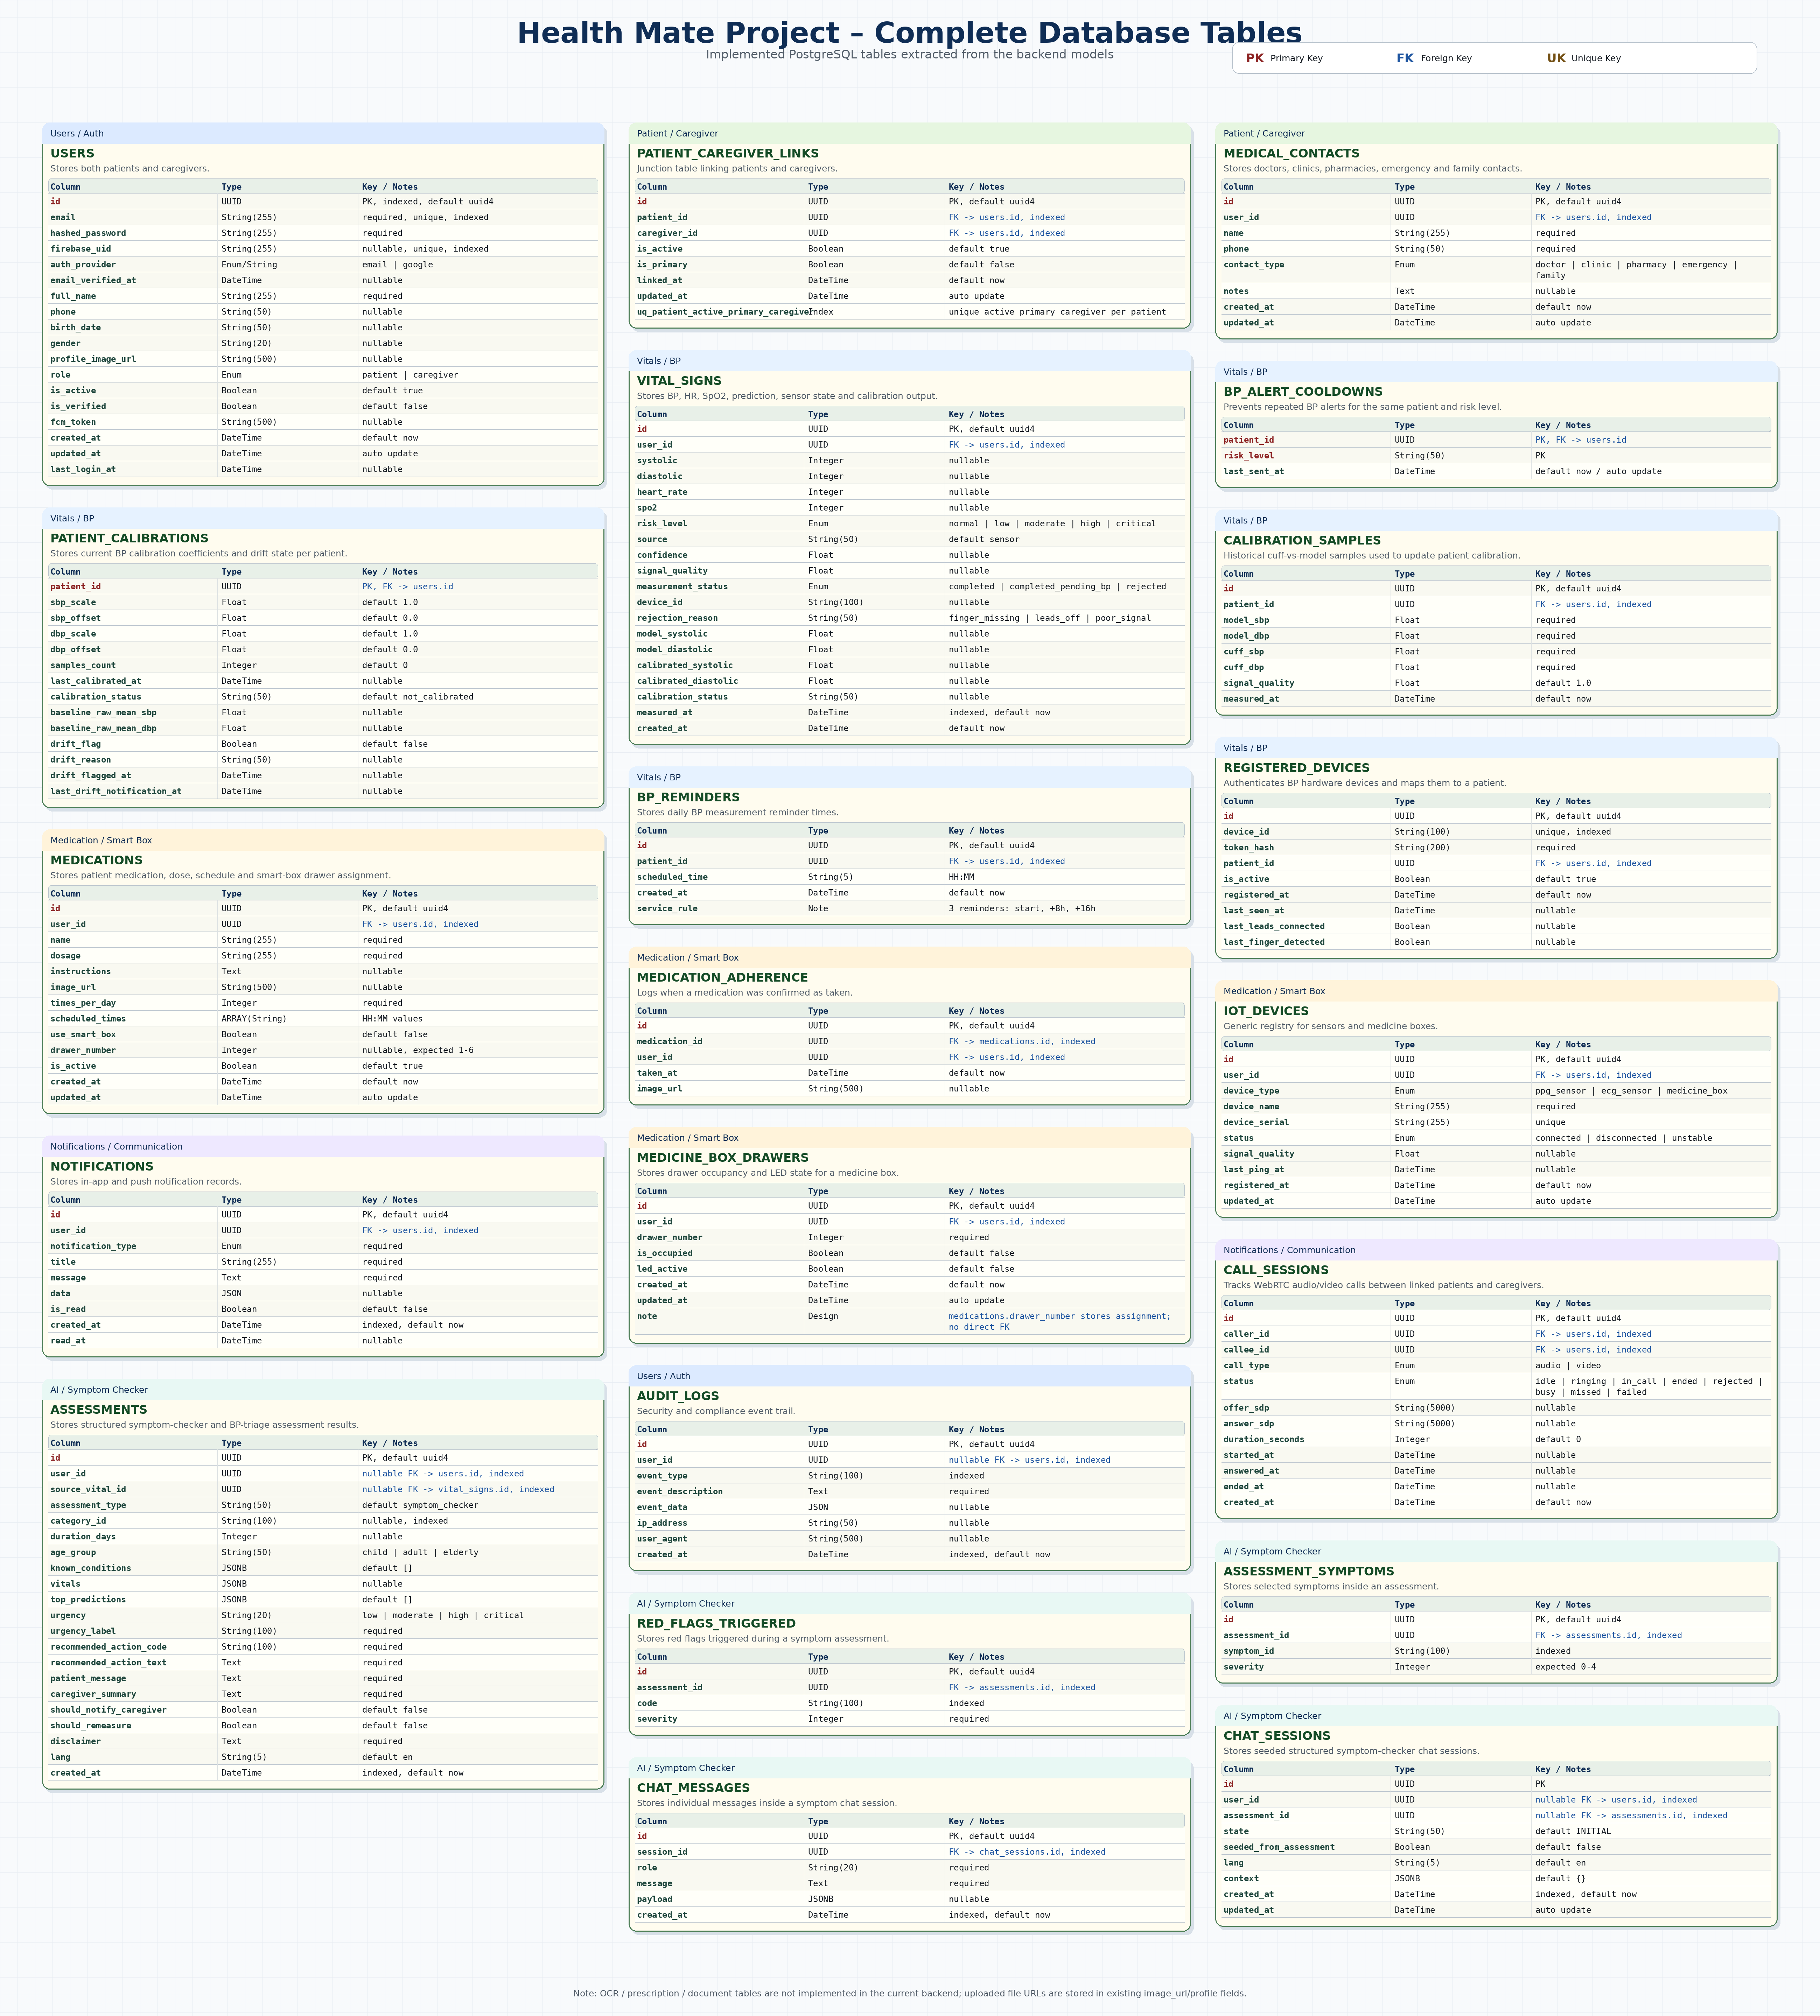
\includegraphics[width=0.98\linewidth,height=0.86\textheight,keepaspectratio]{health_mate_full_database_tables.png}
\caption{Complete database tables reference exported from the implemented
backend models.}
\label{fig:full-db-tables}
\end{figure}
\clearpage

\section{Relationships Worth Calling Out}

\begin{itemize}[leftmargin=1.4em]
  \item \textbf{One many-to-many junction.} \texttt{patient\_caregiver\_links}
  is the only many-to-many table; every other user-owned table is a
  straightforward one-to-many from \texttt{users}. A partial unique index
  (\texttt{WHERE is\_primary AND is\_active}) enforces at most one active primary
  caregiver per patient --- a real database-level invariant, not just an
  application check.
  \item \textbf{The BP-triage database trace.}
  \texttt{assessments.source\_vital\_id} is a nullable FK straight to
  \texttt{vital\_signs}: when a triage runs off a real BP reading, the resulting
  assessment row links directly back to the vital sign that triggered it.
  \item \textbf{Nullable BP by design.} \texttt{vital\_signs.systolic}/
  \texttt{diastolic} are nullable because a sensor-submitted reading can exist in
  a \texttt{completed\_pending\_bp} state (HR/SpO2 known, BP not yet confirmed)
  before a cuff-confirmed value arrives.
  \item \textbf{Two device-registry tables.} \texttt{iot\_devices} is a generic
  registry used by the mock path, while \texttt{registered\_devices} is the
  table actually used for BP-hardware authentication in production; they do not
  reference each other.
\end{itemize}

\section{Business Rules Encoded in the Schema and Domain Layer}

\begin{table}[H]
\centering
\caption{Key business rules, as encoded in the domain layer.}
\label{tab:rules}
\small
\begin{tabularx}{\linewidth}{@{}>{\raggedright\arraybackslash}p{3.6cm}Y@{}}
\toprule
\textbf{Rule} & \textbf{Definition} \\
\midrule
BP risk tiers & Low $<$ 90/60; Normal 90/60--120/80; Moderate 120--139/80--89; High 140--179/90--119; Critical $\ge$ 180/120 \\
Symptom urgency & Critical if any red flag severity $\ge 3$ or critical vitals; High if any red flag or high vitals; Moderate if $\ge 2$ symptoms at severity $\ge 2$ or known hypertension + elevated vitals; else Low \\
Red flags & Most trigger at severity $\ge 2$; syncope/LOC variants at any severity $\ge 1$ \\
Calibration & $<8$ paired samples $\rightarrow$ median offset only; $\ge 8$ $\rightarrow$ least-squares linear fit; both clamp scale $\in[0.70,1.30]$, offset $\in[-25,+25]$ \\
Calibration drift & Flagged on sustained shift $>$8\,mmHg (SBP) or $>$5\,mmHg (DBP) from baseline, or age $>$90 days; re-notify throttled to once / 14 days \\
Emergency cooldown & 15\,min for critical, 30\,min for high/low, per patient per tier \\
Primary caregiver & One active primary per patient, enforced at the database level \\
\bottomrule
\end{tabularx}
\end{table}


%==============================================================================
\chapter{Methodology}
%==============================================================================

This chapter documents the two AI subsystems end to end: the data they were
built from, how that data was preprocessed and represented, how the models were
trained and compared, and how the trained artifacts were carried into
production. Everything below is drawn from the training notebook, the training
scripts, and the generated artifacts they produced.

\section{Data Collection and Preprocessing}

\subsection{Blood-Pressure Dataset}

The blood-pressure model was trained on a MIMIC-derived cuffless dataset
\cite{mimic3}: twelve \texttt{.mat} files, where each record is a
$[3, N]$ array of synchronized PPG, arterial blood pressure (ABP, the reference
signal), and ECG, originally sampled at 125\,Hz. The ABP channel is an
\emph{invasive arterial-line} reading --- this is genuine ground truth for
blood pressure, though it is arterial-line pressure, not sphygmomanometer cuff
pressure, and the two are not identical in every clinical sense.

Splitting is done at the \textbf{record level}, not the window level, to prevent
information leakage:

\begin{itemize}[leftmargin=1.4em]
  \item 15\% of records held out as test.
  \item Of the remaining 85\%, another 15\% held out as validation.
  \item An explicit no-overlap assertion between the three index sets before
  proceeding.
\end{itemize}

A window-level split would leak adjacent, overlapping windows from the same
patient into both train and test and produce an optimistic accuracy estimate.
After extraction and quality filtering, the final window counts are given in
Table~\ref{tab:splits}; the test set spans 1{,}631 distinct records, later
reused for the per-patient calibration simulation.

\begin{table}[H]
\centering
\caption{Final windowed dataset sizes after record-level splitting and quality
filtering.}
\label{tab:splits}
\begin{tabular}{@{}lr@{}}
\toprule
\textbf{Split} & \textbf{Windows} \\
\midrule
Train & 455{,}596 \\
Validation & 99{,}340 \\
Test & 98{,}079 \\
\midrule
\textbf{Total} & \textbf{653{,}015} \\
\bottomrule
\end{tabular}
\end{table}

\subsubsection{Windowing and Reference Labels}

Each record is bandpass filtered, resampled from 125\,Hz to 100\,Hz, then cut
into 8-second (800-sample) windows with 50\% overlap (step size 400 samples).
For each window:

\begin{itemize}[leftmargin=1.4em]
  \item Systolic/diastolic reference values are derived from the ABP channel
  itself, by peak/trough detection and amplitude averaging --- not from a
  separate cuff reading.
  \item Windows are rejected if peak/trough counts fall outside a plausible
  heart-rate range (40--180\,bpm), or if the derived SBP/DBP fall outside
  plausible bounds (SBP 70--200\,mmHg, DBP 40--130\,mmHg, DBP $<$ SBP required).
  \item A signal-to-noise gate ($-7$\,dB) is applied to the PPG channel; on this
  clean dataset it keeps essentially all windows and acts as a safety net.
\end{itemize}

\subsection{Preprocessing Pipeline}

The same three-step pipeline is applied to every window and --- importantly ---
the exact same functions are reused verbatim in the production inference code,
so there is no drift between training and inference:

\begin{enumerate}[leftmargin=1.6em]
  \item \textbf{Bandpass filter} --- 4th-order Butterworth, 0.5--8\,Hz for PPG
  and 0.5--40\,Hz for ECG (zero-phase \texttt{filtfilt}).
  \item \textbf{Z-score normalization} --- $(x-\mu)/(\sigma+10^{-8})$, per
  window, per channel.
  \item \textbf{Feature extraction} --- 21 hand-crafted features (below), also
  z-scored using a scaler fit only on the training set.
\end{enumerate}

Figures~\ref{fig:pipe-max}--\ref{fig:pipe-ad} show this pipeline applied to
synthetic signals shaped like real MAX30102/AD8232 output, demonstrating that
raw sensor units (ADC counts, with a $\sim$150{,}000 DC offset for the PPG
photodiode and $\sim$512 for the single-ended ECG front-end) collapse onto the
same normalized scale the model was trained on --- a deliberate check performed
before ever wiring up real hardware.

\begin{figure}[H]\centering
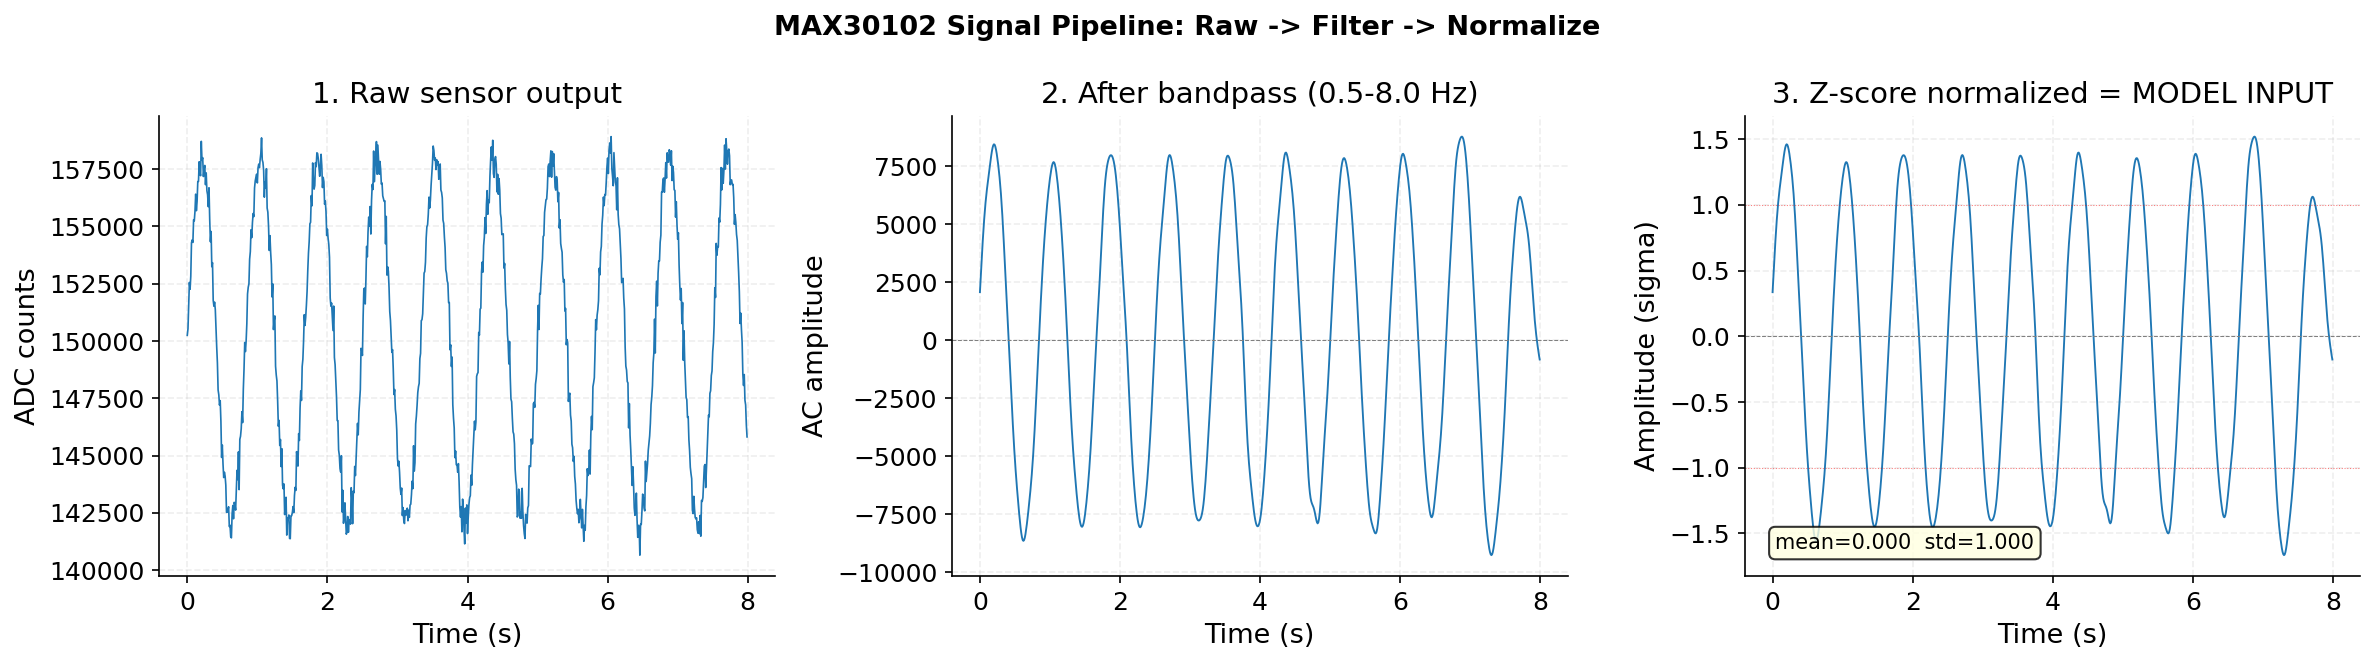
\includegraphics[width=0.92\linewidth]{fig_01_max30102_pipeline.png}
\caption{PPG (MAX30102) preprocessing pipeline: raw ADC counts $\rightarrow$
bandpass $\rightarrow$ z-score normalized.}
\label{fig:pipe-max}\end{figure}

\begin{figure}[H]\centering
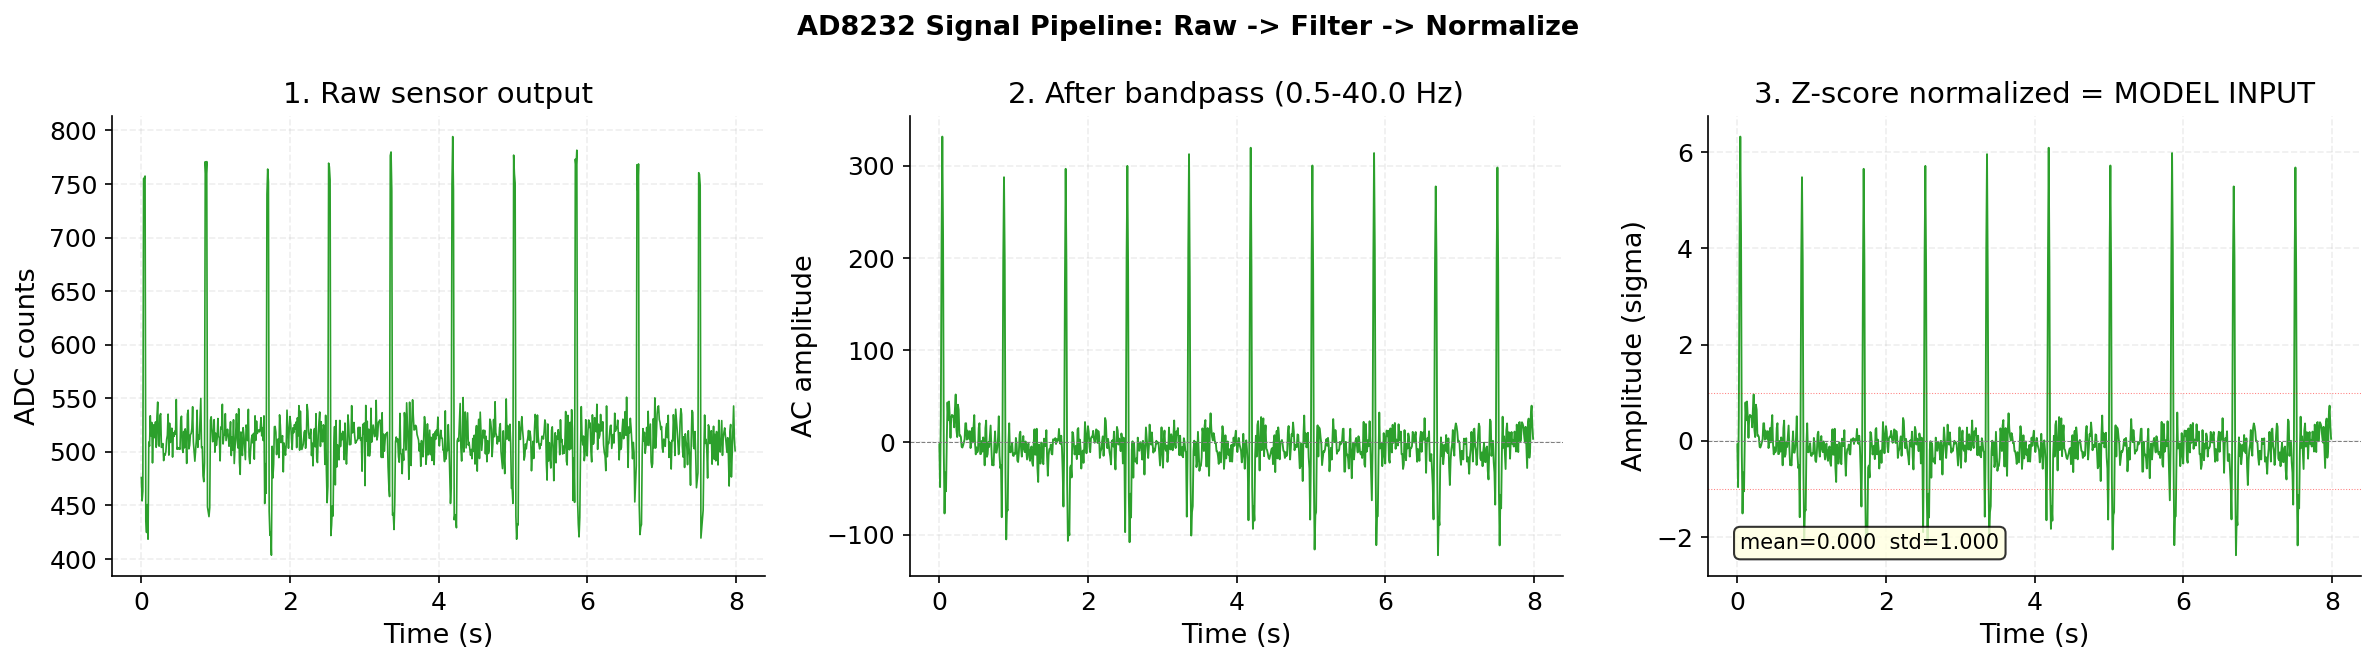
\includegraphics[width=0.92\linewidth]{fig_02_ad8232_pipeline.png}
\caption{ECG (AD8232) preprocessing pipeline: raw single-ended output
$\rightarrow$ bandpass $\rightarrow$ z-score normalized.}
\label{fig:pipe-ad}\end{figure}

\subsection{Feature Engineering}
\label{sec:bpfeatures}

Alongside the raw waveform, a 21-dimensional hand-crafted feature vector is
computed per window and fed into a small dense side-branch
(Table~\ref{tab:bpfeatures}). Pulse transit time (PTT) is the feature most
grounded in physiology --- it is the classical basis for cuffless BP estimation
\cite{kachuee2015}. The notebook's correlation analysis
(Figure~\ref{fig:featcorr}) confirms that PTT and heart rate carry the strongest
linear correlation with SBP/DBP among the 21 features, though none individually
correlates strongly enough to justify a pure feature-based (non-waveform) model.

\begin{table}[H]
\centering
\caption{The 21 hand-crafted features fed to the model's dense side-branch.}
\label{tab:bpfeatures}
\small
\begin{tabularx}{\linewidth}{@{}>{\raggedright\arraybackslash}p{1.3cm}>{\raggedright\arraybackslash}p{4.4cm}Y@{}}
\toprule
\textbf{Index} & \textbf{Feature(s)} & \textbf{Description} \\
\midrule
0--2 & HR\_bpm, RR\_mean\_s, RR\_std\_s & Heart rate and RR-interval statistics from PPG peaks \\
3--4 & PTT\_mean\_s, PTT\_std\_s & Pulse transit time: PPG peak minus preceding ECG R-peak \\
5 & PPG\_rise\_time\_s & Time from preceding trough to peak \\
6--7 & PPG\_amp\_mean, PPG\_amp\_std & Pulse amplitude (peak $-$ preceding trough) \\
8--11 & PPG\_mean/std/skew/kurt & Basic PPG waveform statistics \\
12--13 & VPG\_mean, VPG\_std & First derivative of PPG (velocity plethysmogram) \\
14--15 & APG\_mean, APG\_std & Second derivative of PPG (acceleration plethysmogram) \\
16--17 & ECG\_RR\_mean\_s, ECG\_RR\_std\_s & RR interval from ECG R-peaks \\
18 & ECG\_QRS\_width\_s & Approximate QRS width around each R-peak \\
19--20 & ECG\_mean, ECG\_std & Basic ECG waveform statistics \\
\bottomrule
\end{tabularx}
\end{table}

\begin{figure}[H]\centering
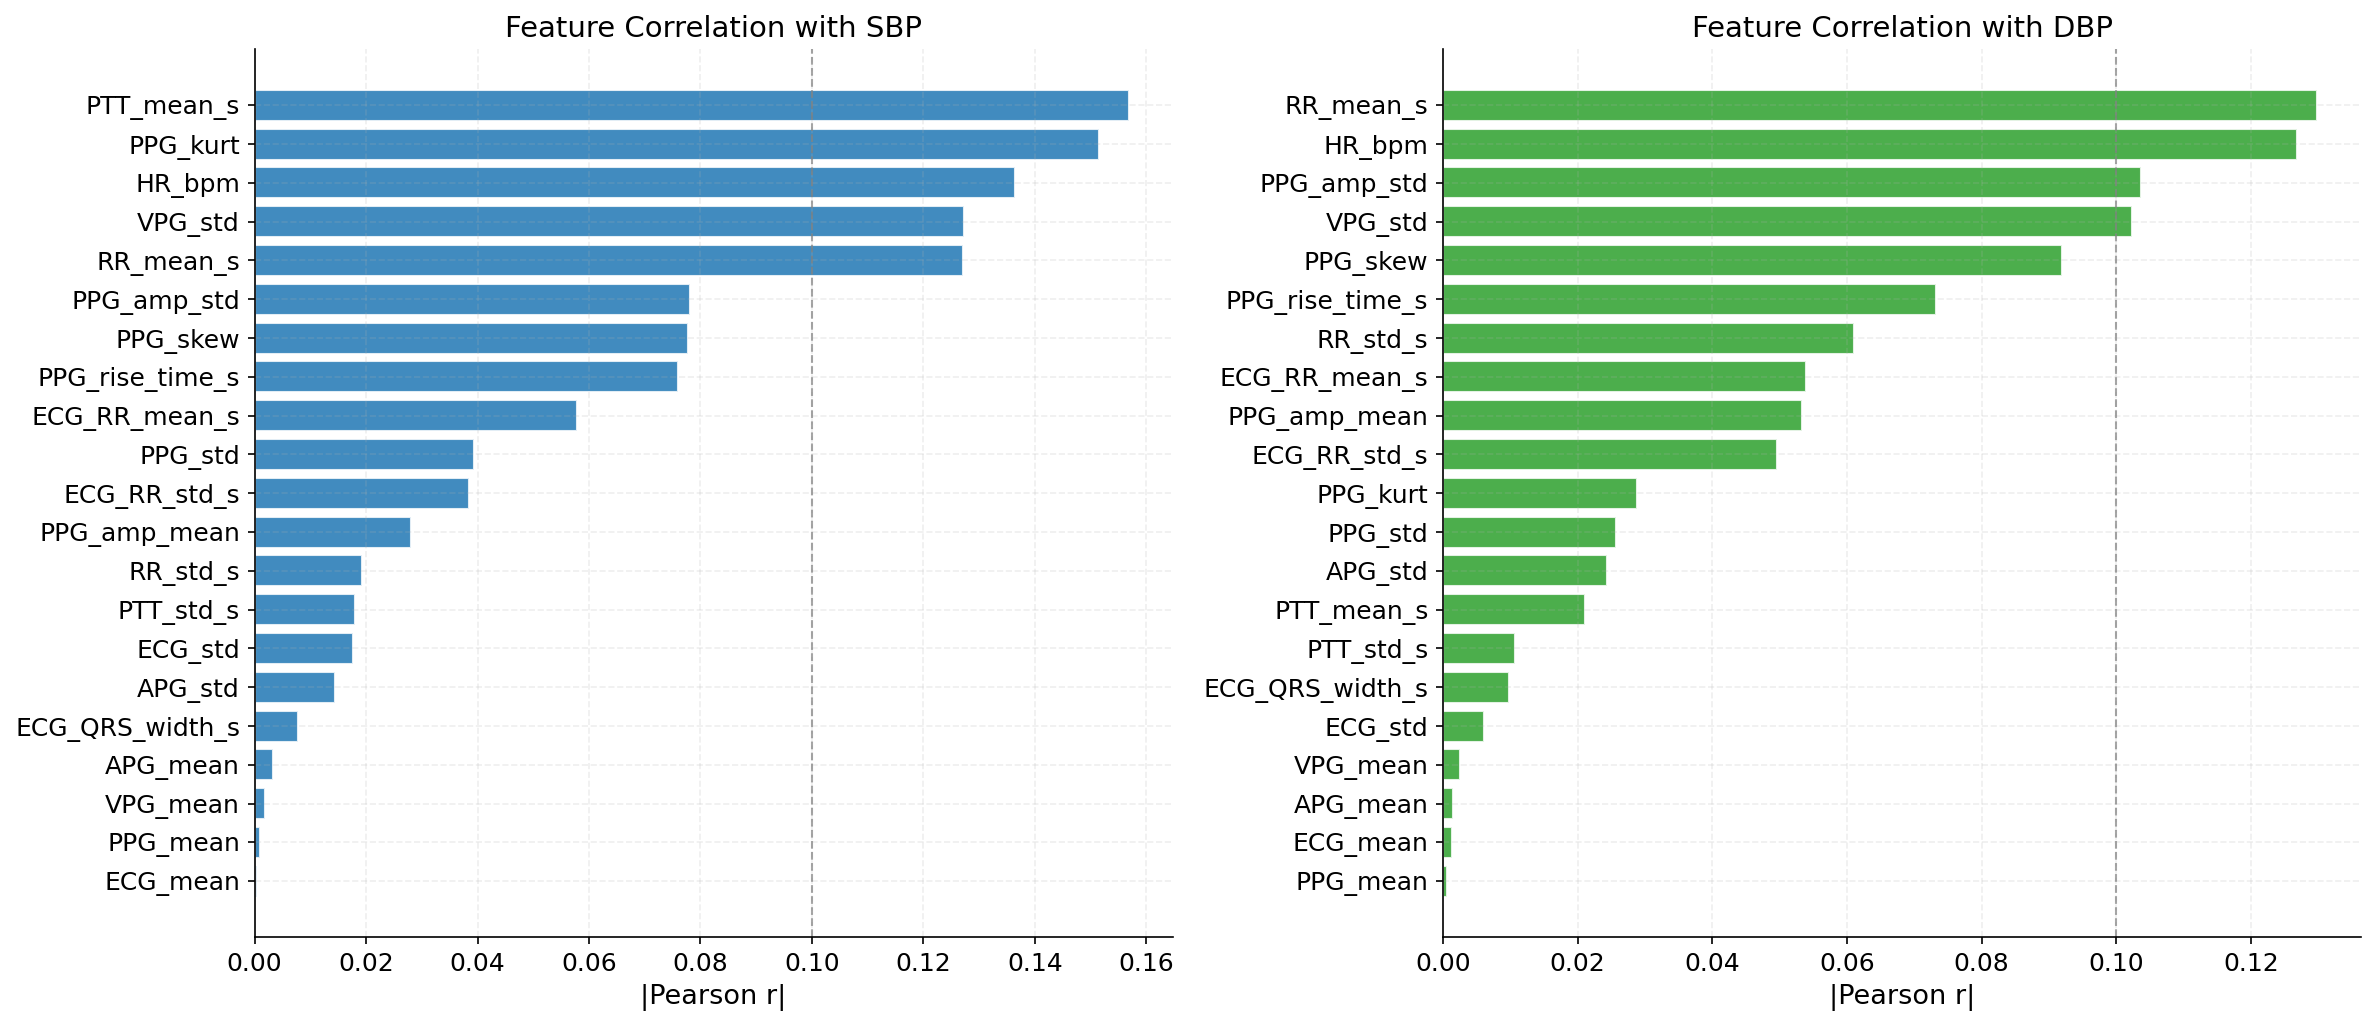
\includegraphics[width=0.82\linewidth]{fig_05_feature_correlation.png}
\caption{Correlation of the 21 hand-crafted features with SBP/DBP. PTT and
heart rate dominate, but no single feature is strong enough on its own.}
\label{fig:featcorr}\end{figure}

\subsection{Class Imbalance: Sample Weights, Not Downsampling}

Windows are labeled into four BP categories (Hypotension, Normal, Elevated,
Hypertension). These are heavily imbalanced (Figure~\ref{fig:bpdist}). An
earlier internal attempt (``v10'') forced class balance by discarding windows
down to 50\,K per class, which threw away most of the real dataset and made the
model \emph{worse} (SBP MAE 11.47 versus an earlier unbalanced 9.13). The final
approach instead computes a per-window sample weight from inverse class
frequency, clipped to a maximum 5$\times$ ratio (Figure~\ref{fig:classw}), and
keeps every real window.

\begin{figure}[H]
\centering
\begin{minipage}{0.48\linewidth}\centering
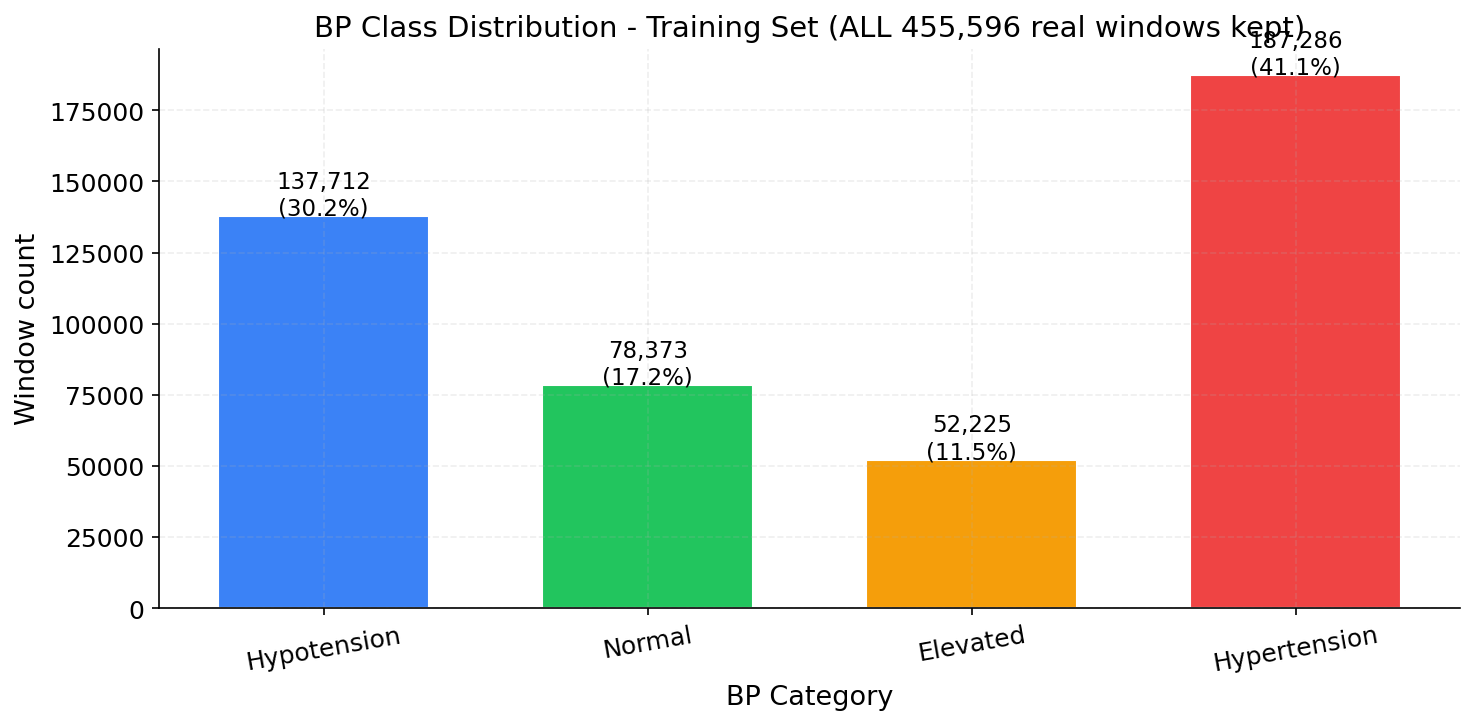
\includegraphics[width=\linewidth]{fig_03_bp_distribution.png}
\captionof{figure}{BP-category distribution: heavily imbalanced toward the
Hypertension and Hypotension extremes.}
\label{fig:bpdist}
\end{minipage}\hfill
\begin{minipage}{0.48\linewidth}\centering
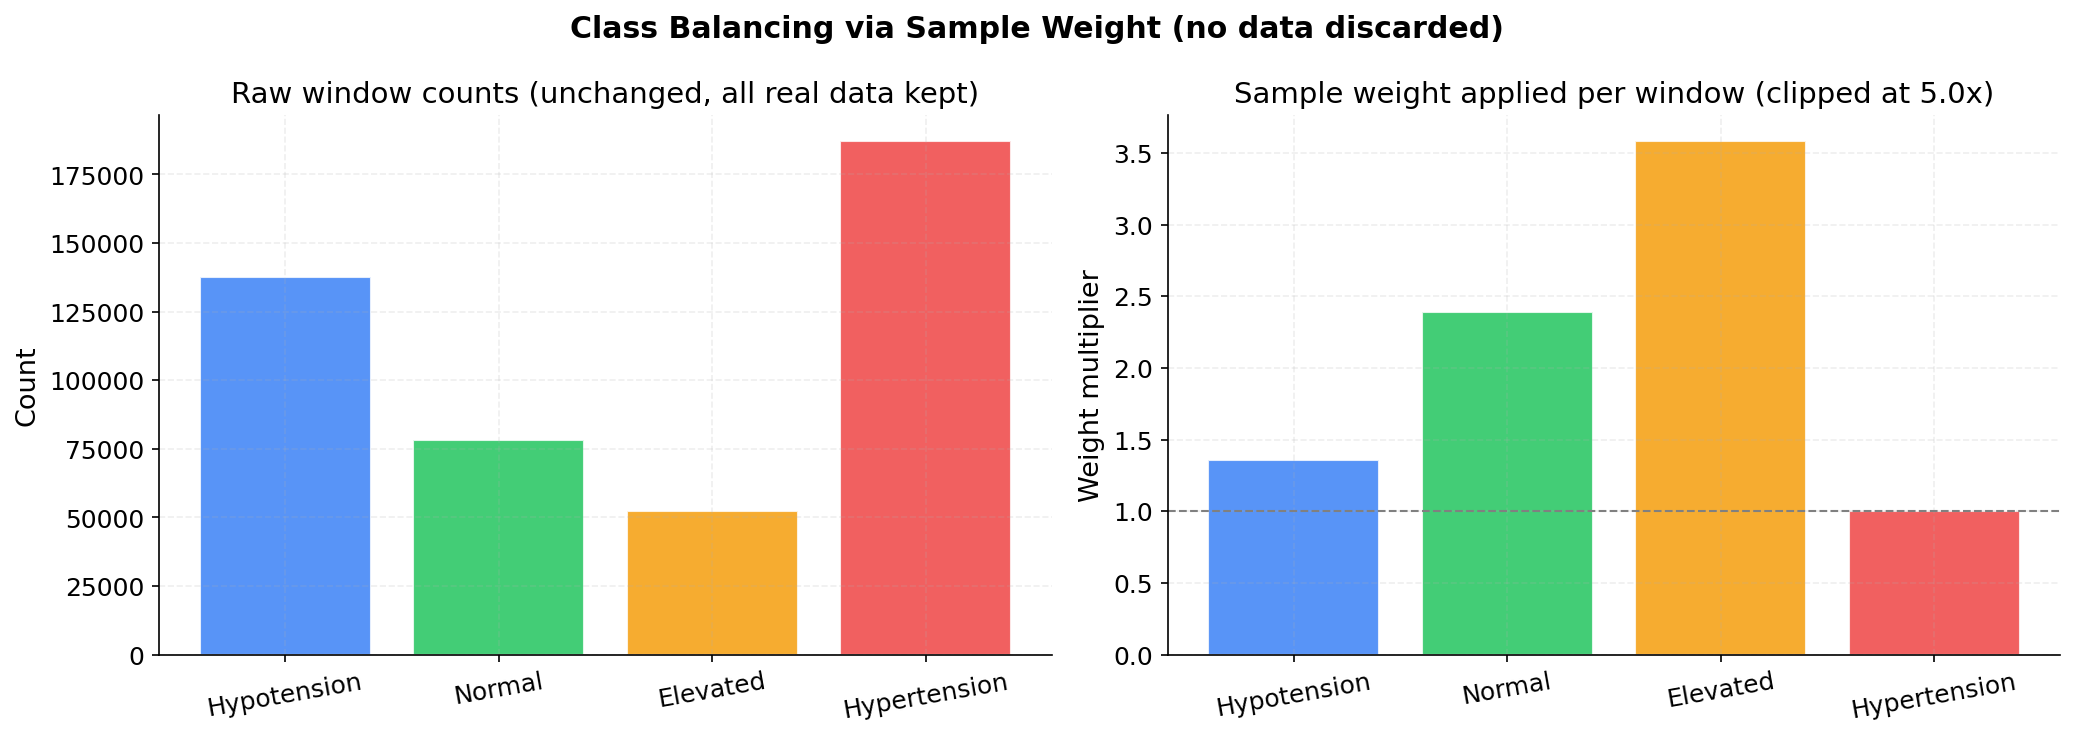
\includegraphics[width=\linewidth]{fig_04_class_weights.png}
\captionof{figure}{Inverse-frequency sample weights, clipped to a 5$\times$
maximum ratio.}
\label{fig:classw}
\end{minipage}
\end{figure}

\subsection{Data Augmentation}

A modest synthetic augmentation (15\% of the real training-set size, versus 40\%
in the earlier ``v10'' attempt) is layered on top of the full real dataset,
using three sensor-realistic perturbations applied together per augmented
sample: additive white Gaussian noise (target SNR 25\,dB), slow baseline wander
(0.05--0.3\,Hz sinusoid, random phase/amplitude), and random amplitude scaling
(0.8--1.2$\times$ for PPG, 0.85--1.15$\times$ for ECG). This adds 68{,}339
synthetic windows on top of the 455{,}596 real ones, for an effective training
set of 523{,}935 windows, shuffled so real and synthetic windows interleave.

\subsection{Symptom-Checker Dataset}

The structured (v2) symptom model's training data is explicitly \textbf{synthetic},
generated from a taxonomy of diseases, symptoms, and categories rather than
collected from real patients:

\begin{itemize}[leftmargin=1.4em]
  \item Each disease's related-symptom list becomes a symptom-inclusion
  probability profile (symptoms listed earlier get higher probability, from
  0.85 down to a 0.35 floor).
  \item Each synthetic case independently samples severity, duration, age
  group, and optional risk factors/vitals around that profile.
  \item A target of 300 cases per disease is generated, split into 9{,}840
  train / 2{,}460 test at training time across 40 disease classes.
  \item \textbf{Urgency labels are not hand-assigned} --- every generated case
  is run through the same production rule engine that judges real assessments,
  so the dataset can never encode an urgency value that disagrees with the
  live logic.
  \item Targeted differentiation was applied to two commonly-confused clusters:
  Common Cold / Influenza / COVID-19 (separated by duration, severity, and a
  boosted probability of loss of taste/smell for COVID-19), and Hypertension /
  Migraine / Stroke (whose symptom sets already do not overlap in the taxonomy).
\end{itemize}

The resulting per-case representation is a 232-dimension feature vector, a
single \texttt{build\_features()} function shared verbatim between training and
production inference (Table~\ref{tab:symfeatures}).

\begin{table}[H]
\centering
\caption{Layout of the 232-dimension structured symptom feature vector.}
\label{tab:symfeatures}
\small
\begin{tabularx}{\linewidth}{@{}>{\raggedright\arraybackslash}p{3.3cm}>{\raggedright\arraybackslash}p{2.2cm}Y@{}}
\toprule
\textbf{Segment} & \textbf{Size} & \textbf{Content} \\
\midrule
Symptom presence & $N_{sym}$ & Multi-hot: 1 if the symptom was selected \\
Symptom severity & $N_{sym}$ & 0 if absent, else the reported severity \\
Duration bucket & 4 & One-hot: $<$1, 1--3, 4--7, $>$7 days \\
Age group & 3 & One-hot: child / adult / elderly \\
Risk factors & 5 & Multi-hot over a comorbidity pool (hypertension, T2 diabetes, asthma, hypothyroidism, CKD) \\
Vitals & 4 & Normalized systolic/diastolic/heart rate (clipped) + a \texttt{vitals\_present} flag \\
\bottomrule
\end{tabularx}
\end{table}

\section{Model Development}

\subsection{Blood-Pressure Models}

Ten models were trained and evaluated on the identical test set, all using the
same 21 features (classical) or the same waveform + feature combination (deep
learning), and all trained with the same sample weights:

\begin{itemize}[leftmargin=1.4em]
  \item \textbf{Classical ML (6):} Ridge, ElasticNet, Random Forest, XGBoost,
  LightGBM, CatBoost --- each predicting SBP/DBP jointly.
  \item \textbf{Deep learning (4):} 1D-CNN, BiLSTM, TCN, and the team's proposed
  TCN+BiLSTM+Attention model. All four share a two-branch design: a waveform
  encoder consuming the raw $(800,2)$ PPG+ECG tensor, and a small dense branch
  consuming the 21 features, concatenated before a shared prediction head
  (Table~\ref{tab:dlmodels}).
\end{itemize}

\begin{table}[H]
\centering
\caption{The four deep-learning architectures and their parameter counts.}
\label{tab:dlmodels}
\small
\begin{tabularx}{\linewidth}{@{}>{\raggedright\arraybackslash}p{4.0cm}Yr@{}}
\toprule
\textbf{Model} & \textbf{Encoder} & \textbf{Params} \\
\midrule
1D-CNN & 4-stage Conv1D + MaxPooling, global average pool & 485{,}154 \\
BiLSTM & 2 Conv+Pool stages (800$\rightarrow$50 steps) feeding a bidirectional LSTM & 371{,}234 \\
TCN & 4-stage dilated causal Conv1D residual blocks (dilations 1/2/4/8) & 1{,}017{,}634 \\
TCN+BiLSTM+Attn (ours) & TCN $\rightarrow$ BiLSTM $\rightarrow$ 4-head self-attention $\rightarrow$ residual + LayerNorm & 1{,}544{,}610 \\
\bottomrule
\end{tabularx}
\end{table}

The conceptual two-branch design and the best model's exact Keras layer graph
are shown in Figures~\ref{fig:modeloverview}--\ref{fig:keras1dcnn}, and the exact
auto-generated layer graphs of the other three architectures (BiLSTM, TCN, and
the team's full TCN+BiLSTM+Attention model) are shown together in
Figure~\ref{fig:keras3}. Each architecture's graph was produced directly by
Keras \texttt{plot\_model} on the trained model, so these are the real,
verifiable network structures, not redrawn approximations. The BiLSTM
architecture is worth calling out: an earlier version ran the LSTM directly over
all 800 raw timesteps and was the slowest model in the ablation (64\,ms/step);
the current version downsamples to 50 steps with two Conv+Pool stages first ---
a documented performance fix, not an incidental choice.

\begin{figure}[H]
\centering
\begin{minipage}{0.46\linewidth}\centering
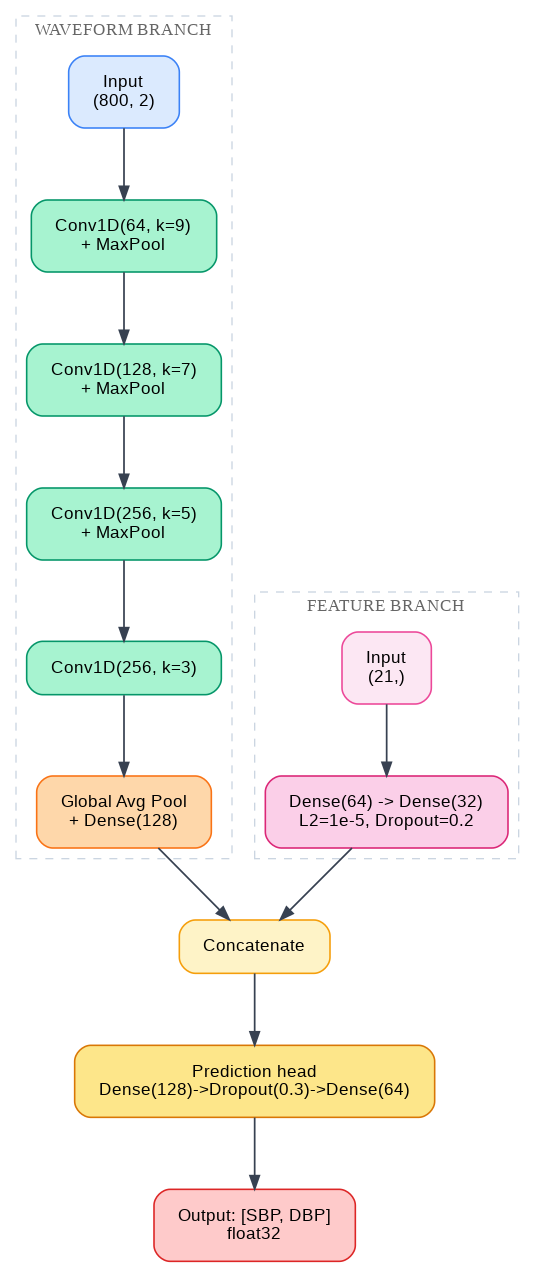
\includegraphics[height=8.2cm]{fig_31_model_architecture_overview.png}
\captionof{figure}{Conceptual two-branch design: a waveform encoder and a dense
feature branch, concatenated before a shared prediction head.}
\label{fig:modeloverview}
\end{minipage}\hfill
\begin{minipage}{0.46\linewidth}\centering
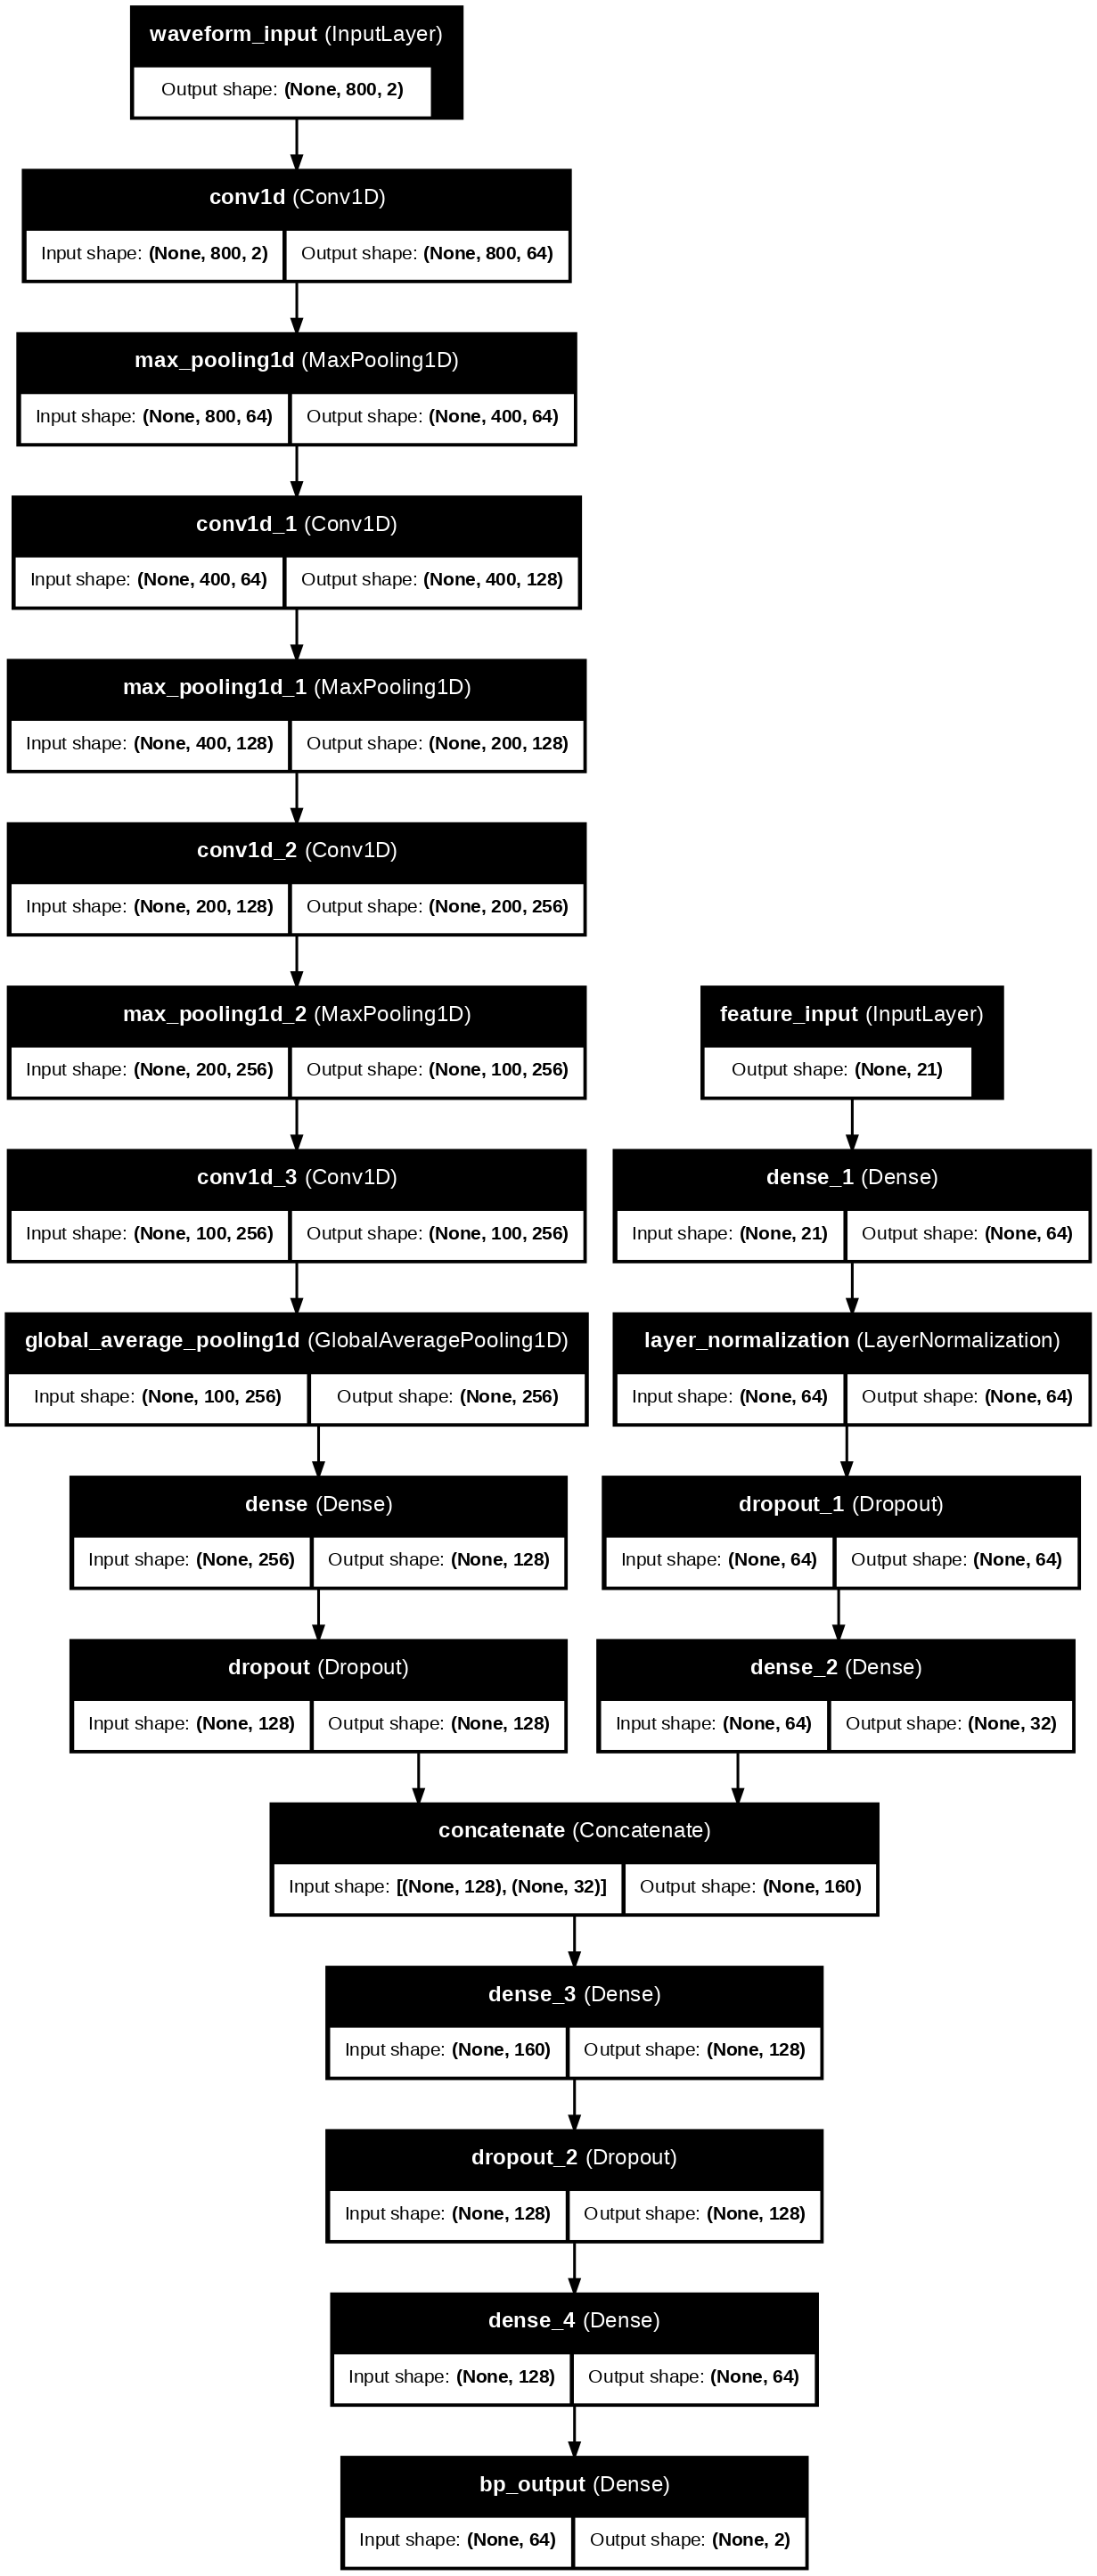
\includegraphics[height=8.2cm]{fig_32_keras_1d_cnn.png}
\captionof{figure}{Exact Keras layer graph of the best-performing 1D-CNN model
(auto-generated by \texttt{plot\_model}).}
\label{fig:keras1dcnn}
\end{minipage}
\end{figure}

\begin{figure}[H]
\centering
\begin{minipage}{0.30\linewidth}\centering
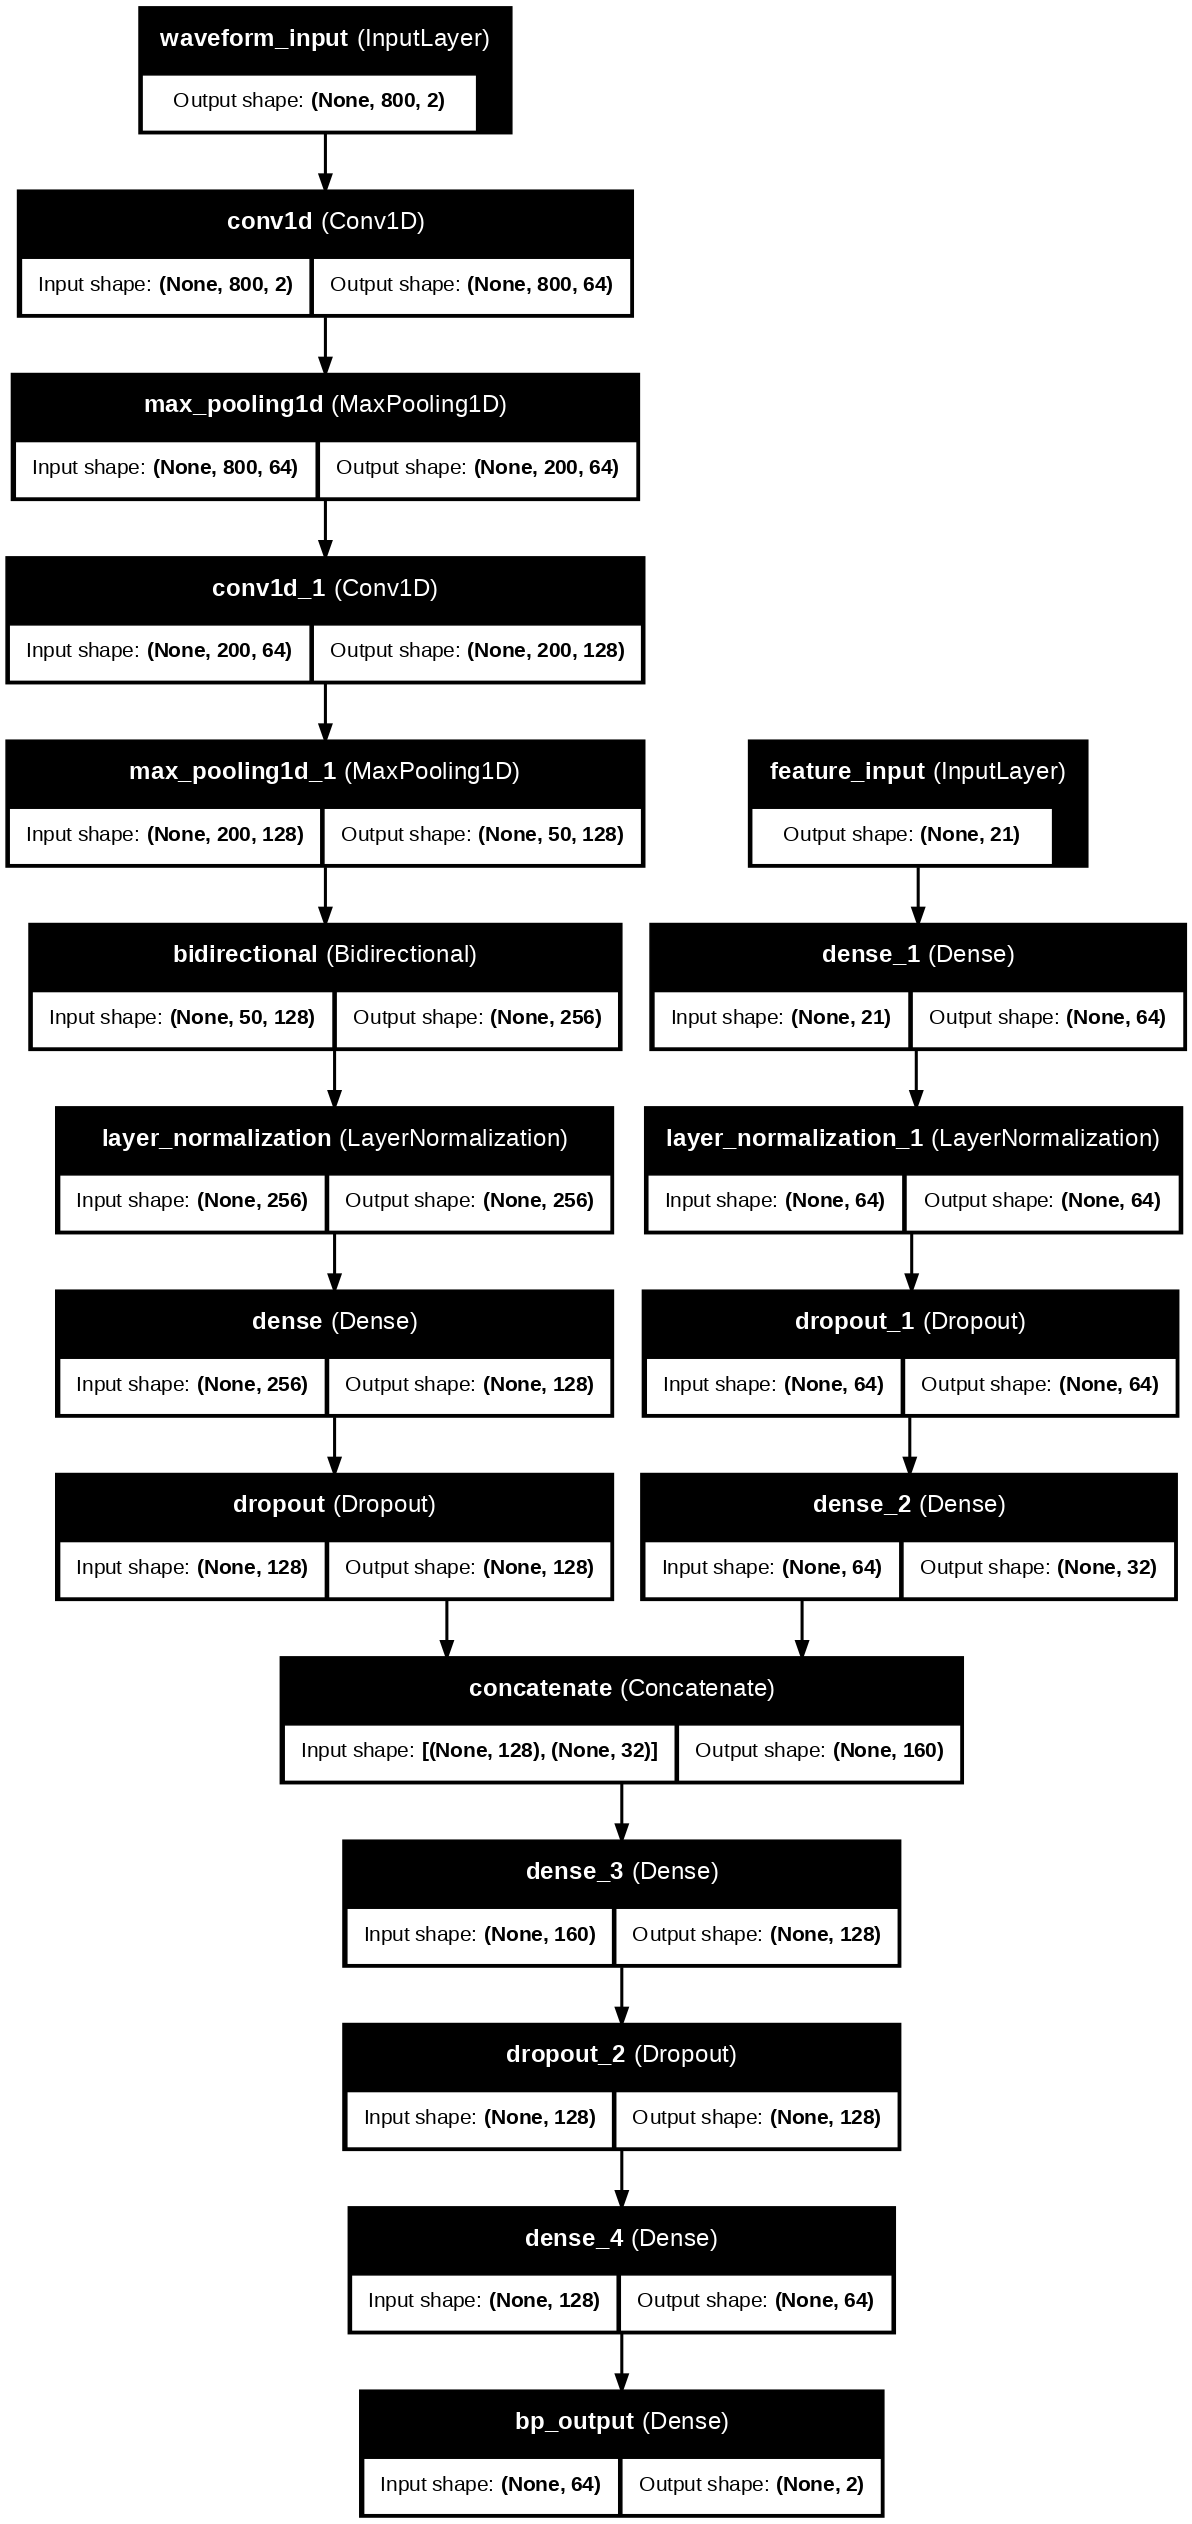
\includegraphics[height=8.6cm]{fig_33_keras_bilstm.png}\\[2pt]
{\scriptsize (a) BiLSTM}
\end{minipage}\hfill
\begin{minipage}{0.30\linewidth}\centering
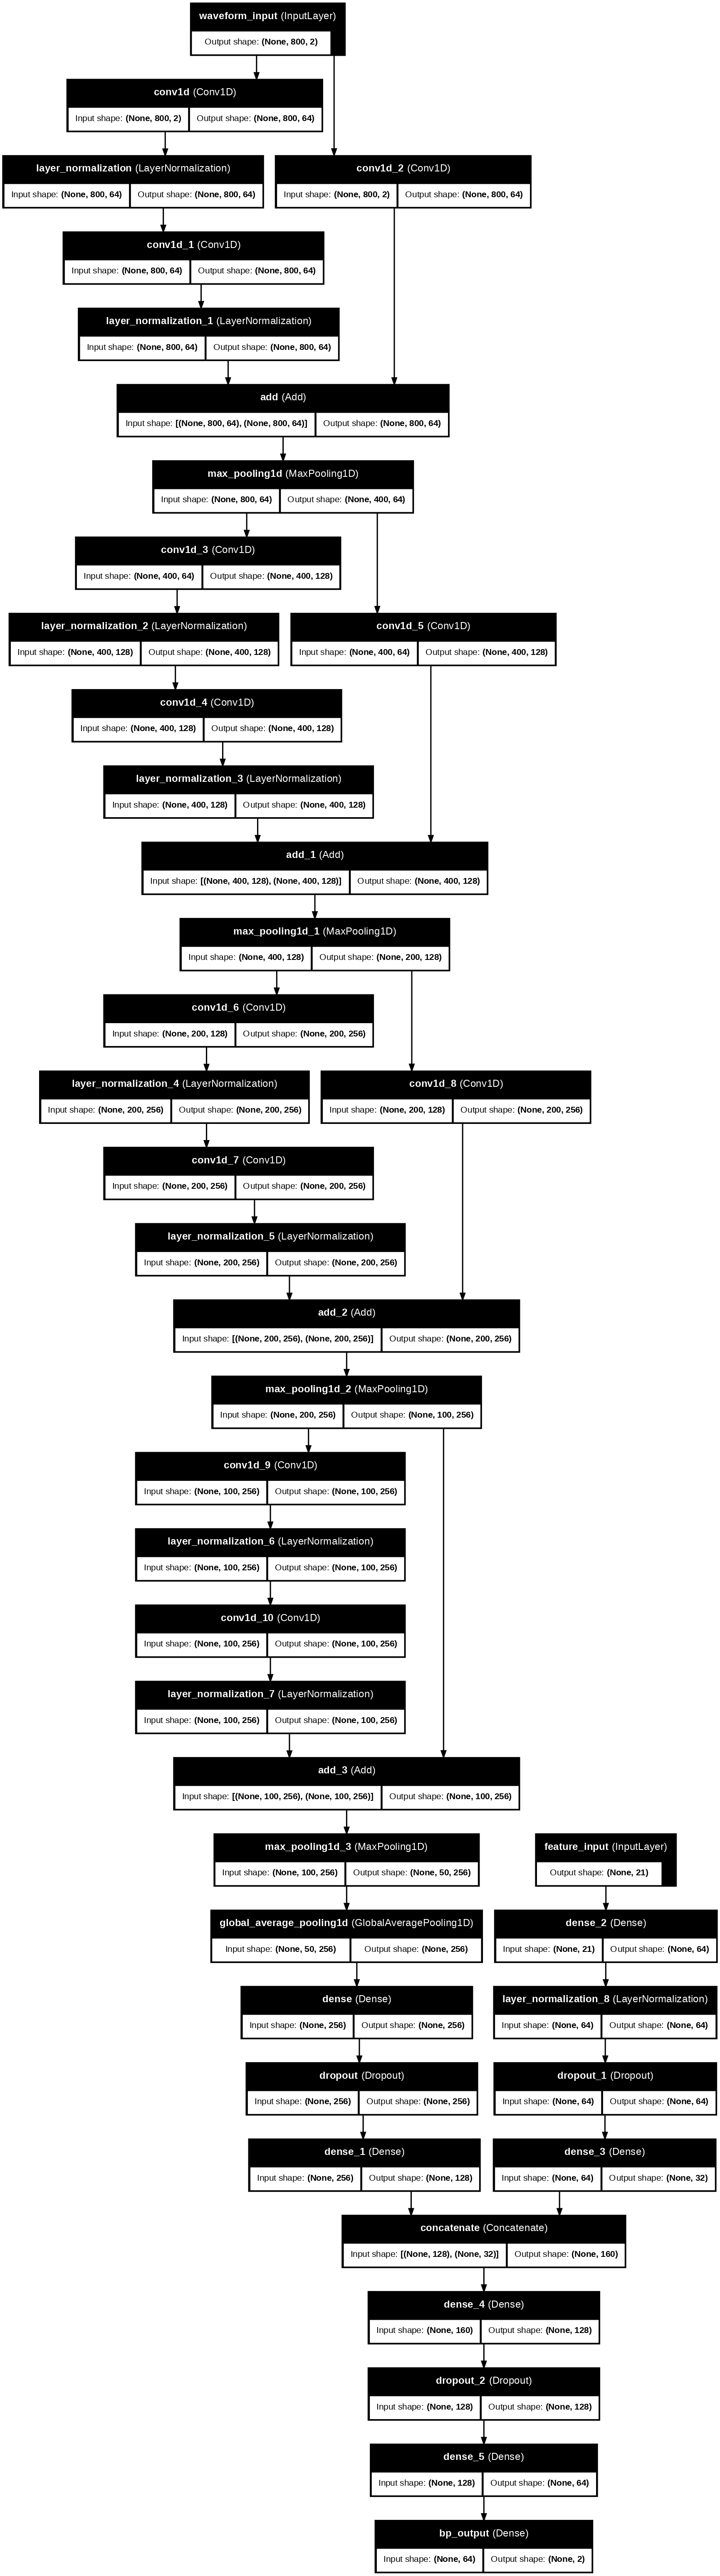
\includegraphics[height=8.6cm]{fig_34_keras_tcn.png}\\[2pt]
{\scriptsize (b) TCN}
\end{minipage}\hfill
\begin{minipage}{0.30\linewidth}\centering
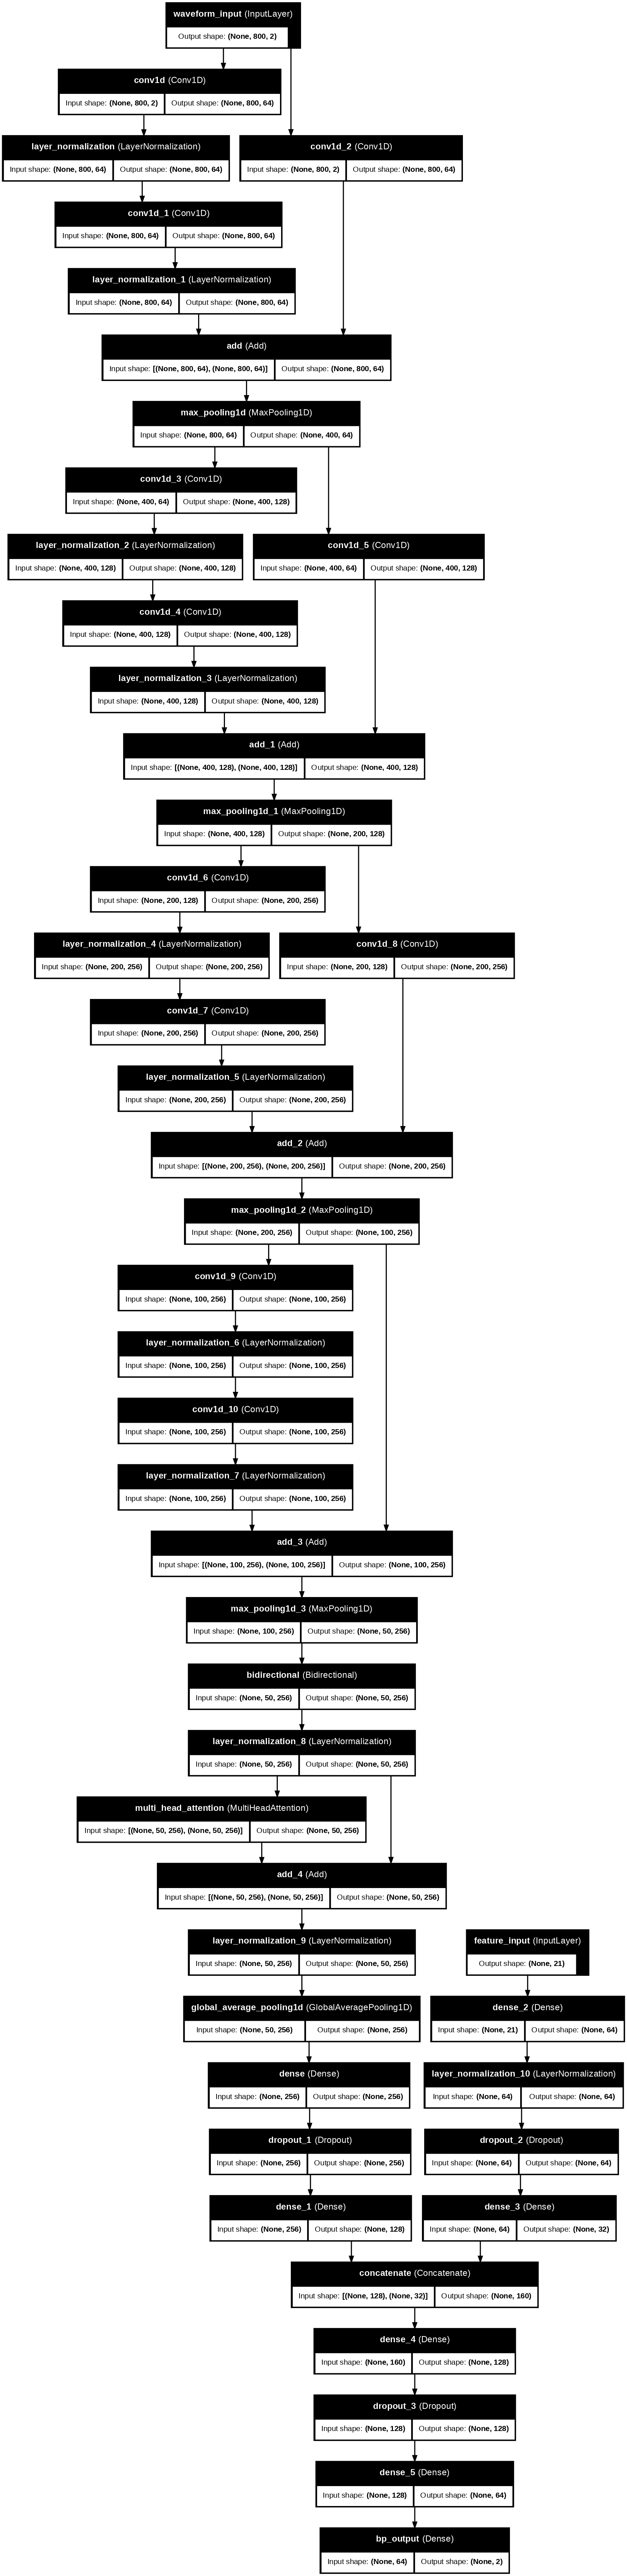
\includegraphics[height=8.6cm]{fig_35_keras_full_model.png}\\[2pt]
{\scriptsize (c) TCN+BiLSTM+Attn (ours)}
\end{minipage}
\caption{Exact Keras layer graphs of the other three deep-learning
architectures. The increasing depth from (a) to (c) reflects the rising
parameter counts in Table~\ref{tab:dlmodels} --- and, as the results show, that
added depth did not translate into better accuracy.}
\label{fig:keras3}
\end{figure}

\subsubsection{Regularization: a Documented Course-Correction}

The notebook explicitly documents why the current hyperparameters differ from an
earlier attempt (``v4''): v4 used \emph{no} L2 regularization, producing an 86\%
train/validation MAE gap (severe overfitting). The current configuration uses
light L2 ($10^{-5}$) and 0.3 dropout, bringing the healthiest models'
overfitting gap down substantially (Figure~\ref{fig:overfit}). A dead decoder
branch (from an abandoned reconstruction loss that never moved during training)
was also removed. Training uses Huber loss (robust to noisy windows), Adam with
gradient clipping, learning-rate reduction on plateau, and early stopping on
validation MAE with best-weight restoration, on a dual-T4 Kaggle session with
mixed precision.

\begin{figure}[H]\centering
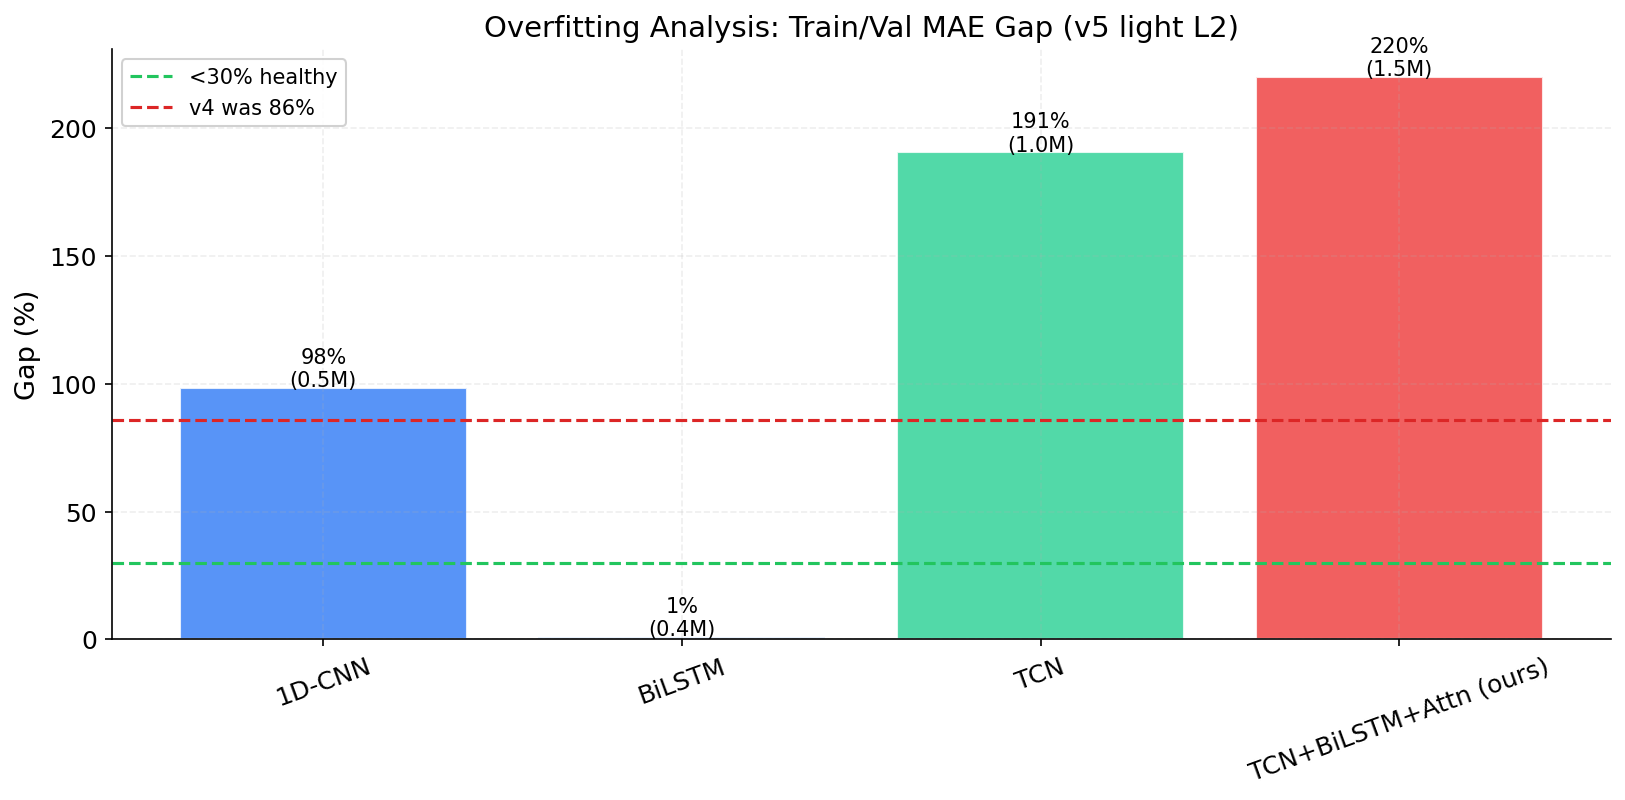
\includegraphics[width=0.85\linewidth]{fig_16_overfitting_analysis.png}
\caption{Train-versus-validation MAE gap across models after the regularization
course-correction.}
\label{fig:overfit}\end{figure}

\subsubsection{Fault Tolerance and Reproducibility}

Every expensive stage --- window extraction, feature engineering, and each
model's training --- checkpoints to disk. If the session is interrupted (a real
risk on free Kaggle GPU quotas) and restarted, completed stages are detected
from cached files and skipped. Each model is wrapped in its own try/except, so
one model crashing does not take down the run. This resumable design
(Figure~\ref{fig:trainflow}) is what made training practical across multiple
sessions on a shared, quota-limited GPU.

\begin{figure}[H]\centering
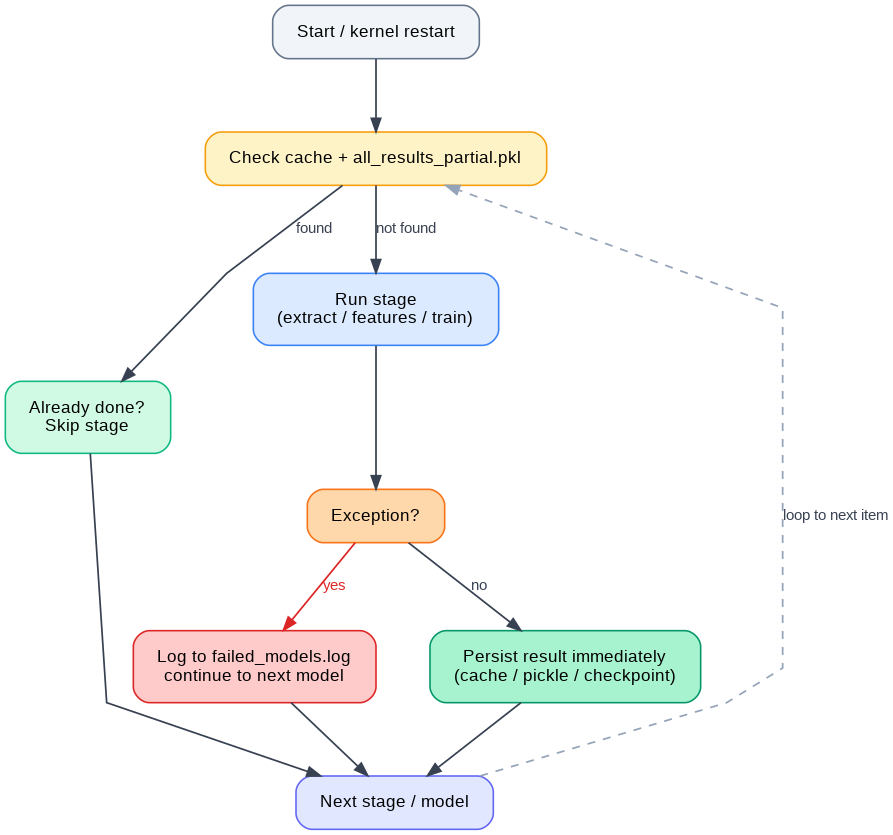
\includegraphics[width=0.6\linewidth]{fig_36_training_workflow.png}
\caption{Fault-tolerant, resumable training workflow: cache-and-resume at every
stage, with per-model isolation.}
\label{fig:trainflow}\end{figure}

\subsection{Symptom-Checker Model}

The production candidate is a LightGBM classifier~\cite{lightgbm} with a
multiclass objective, 300 estimators, learning rate 0.05, over the 40 disease
classes and the 232-feature vector. Two simpler baselines (Logistic Regression,
Random Forest) were trained on the identical feature matrix and split
specifically for comparison --- a decision that turns out to matter
(Section~\ref{sec:symresults}).

\section{Implementation}

The trained BP model's exact preprocessing and inference logic (bandpass filter
$\rightarrow$ z-score normalize $\rightarrow$ feature extraction $\rightarrow$
model call $\rightarrow$ inverse-transform to mmHg) is implemented once in the
training notebook and reimplemented in the backend's inference service using the
identical function bodies. The three exported artifacts ---
\texttt{bp\_model\_final.keras}, \texttt{scaler\_features.pkl}, and
\texttt{scaler\_targets.pkl} --- are copied verbatim into the backend. On top of
the notebook template, the backend service adds:

\begin{itemize}[leftmargin=1.4em]
  \item \textbf{Graceful startup} --- if the model files are missing, the
  service reports \texttt{model\_not\_ready} instead of crashing the API.
  \item \textbf{Input validation} --- exact window length and all-finite checks
  before inference.
  \item \textbf{Physiological clamping} --- output clamped to SBP 50--300, DBP
  30--200, HR 30--220 as a final safety net before any number reaches a patient
  screen.
\end{itemize}

The equivalent guarantee exists on the symptom-checker side: the 232-feature
builder is written once and imported directly by the backend at inference time
(via a runtime cross-directory import), rather than reimplemented, so the
training and inference feature layouts can never silently diverge. Both models
are loaded in-process by the FastAPI backend rather than served by a separate
inference process, each with an explicit ``not ready'' fallback rather than a
crash if artifacts are missing at startup.


%==============================================================================
\chapter{Results and Discussion}\label{sec:results}
%==============================================================================

\section{Model Performance}

\subsection{Blood-Pressure Results}

Table~\ref{tab:bpresults} gives the final test-set metrics for all ten models,
sorted by SBP MAE. Figures~\ref{fig:maesbp}--\ref{fig:maedbp} visualize the same
comparison against the AAMI limit and the internal ``v4'' baseline.

\begin{table}[H]
\centering
\caption{Final test-set results for all ten blood-pressure models, sorted by
SBP MAE. Lower MAE is better; BHS grades run A (best) to D (worst).}
\label{tab:bpresults}
\small
\begin{tabular}{@{}lrcrc@{}}
\toprule
\textbf{Model} & \textbf{SBP MAE} & \textbf{SBP BHS} & \textbf{DBP MAE} & \textbf{DBP BHS} \\
\midrule
\textbf{1D-CNN (best)} & \textbf{9.08} & D & \textbf{4.91} & B \\
TCN & 9.79 & D & 5.31 & B \\
TCN+BiLSTM+Attn (ours) & 10.17 & D & 5.63 & B \\
BiLSTM & 14.34 & D & 7.28 & C \\
XGBoost & 14.71 & D & 7.45 & C \\
CatBoost & 15.13 & D & 7.58 & C \\
LightGBM & 15.16 & D & 7.59 & C \\
Random Forest & 15.80 & D & 7.83 & C \\
Ridge & 18.03 & D & 8.59 & D \\
ElasticNet & 18.37 & D & 8.73 & D \\
\bottomrule
\end{tabular}
\end{table}

Against the reference clinical standards:

\begin{itemize}[leftmargin=1.4em]
  \item \textbf{AAMI SP10} (requires MAE $\le$ 5\,mmHg \emph{and} SD $\le$
  8\,mmHg): every model \emph{fails} this for SBP. The best model (1D-CNN)
  \emph{passes} it for DBP (MAE 4.91, SD 7.77).
  \item \textbf{BHS protocol}~\cite{bhs} grades A--D by the percentage of errors
  within 5, 10, and 15\,mmHg. The best SBP result is Grade D; DBP reaches
  Grade B.
\end{itemize}

The simplest deep-learning architecture --- the plain 1D-CNN --- was the best
performer overall, beating both the TCN and the more elaborate
TCN+BiLSTM+Attention model the team specifically designed for this problem. All
three deep-learning waveform models comfortably outperformed every classical
feature-only model, consistent with the raw waveform carrying information the 21
hand-crafted features alone do not fully capture. The result is documented
as-is; the notebook does not attempt to explain away why the attention model
underperformed, and neither does this document.

\begin{figure}[H]
\centering
\begin{minipage}{0.49\linewidth}\centering
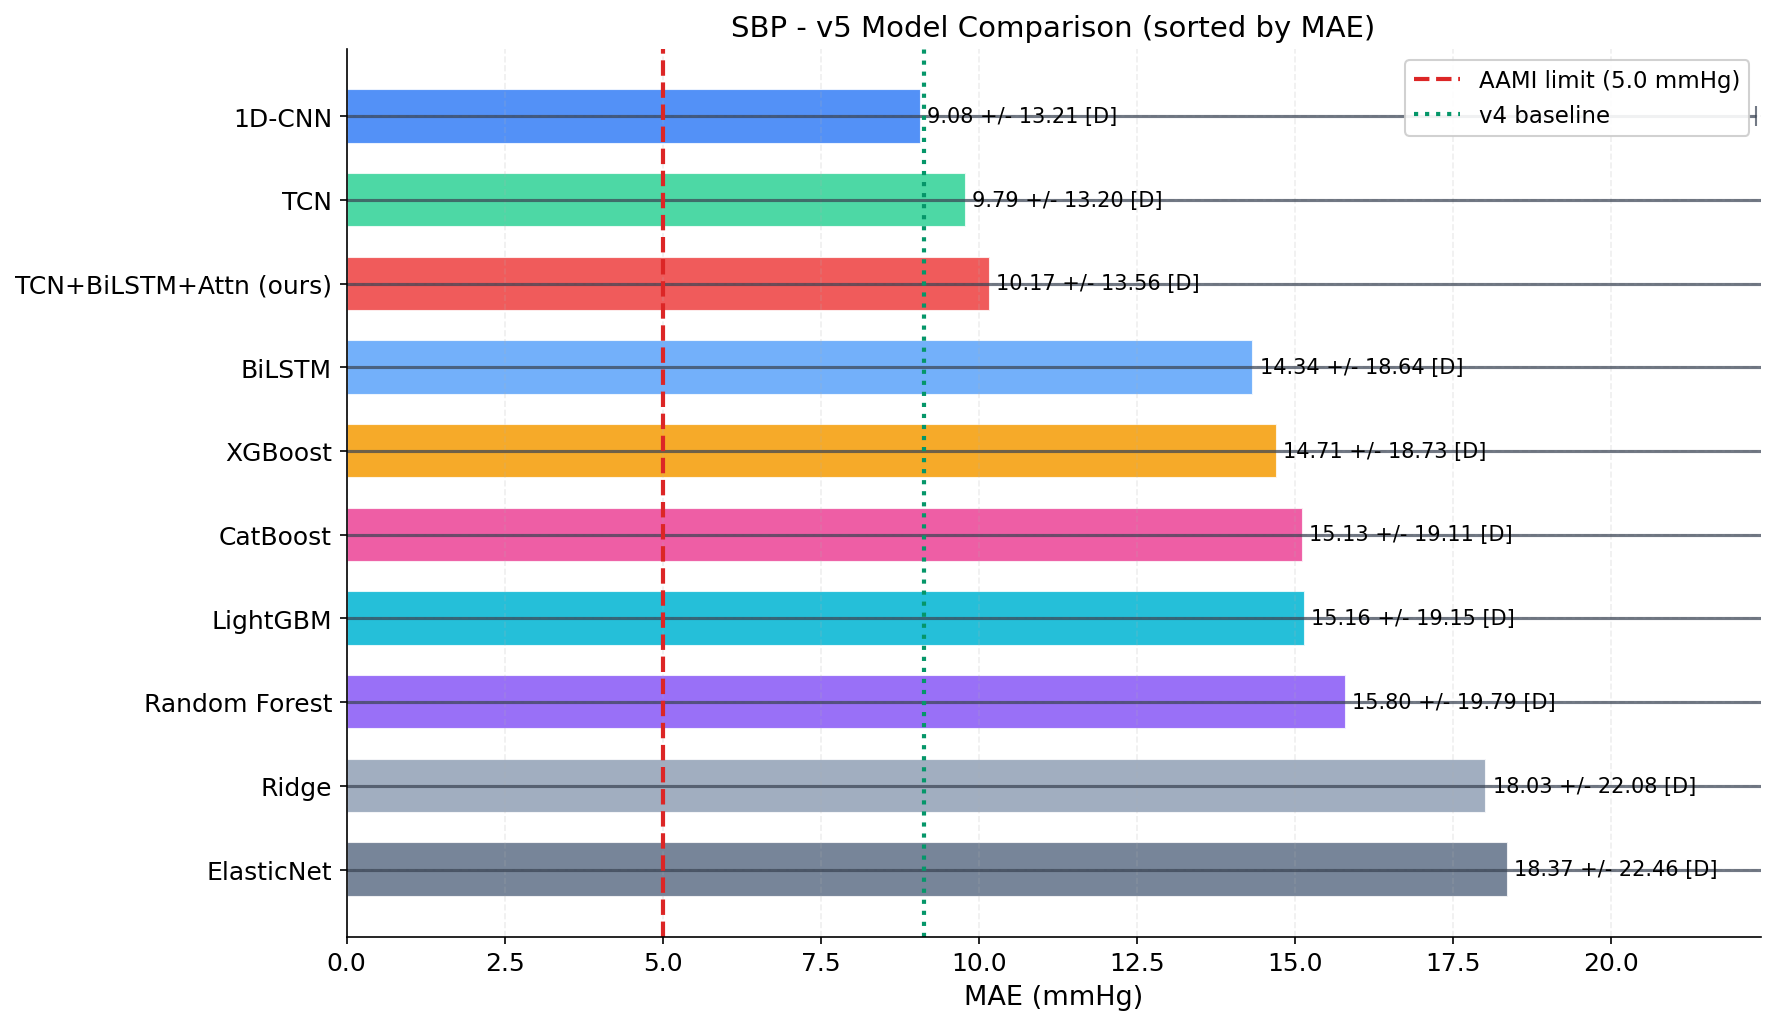
\includegraphics[width=\linewidth]{fig_12_mae_comparison_sbp.png}
\captionof{figure}{SBP MAE across all ten models against the AAMI limit
(5\,mmHg) and the v4 baseline.}
\label{fig:maesbp}
\end{minipage}\hfill
\begin{minipage}{0.49\linewidth}\centering
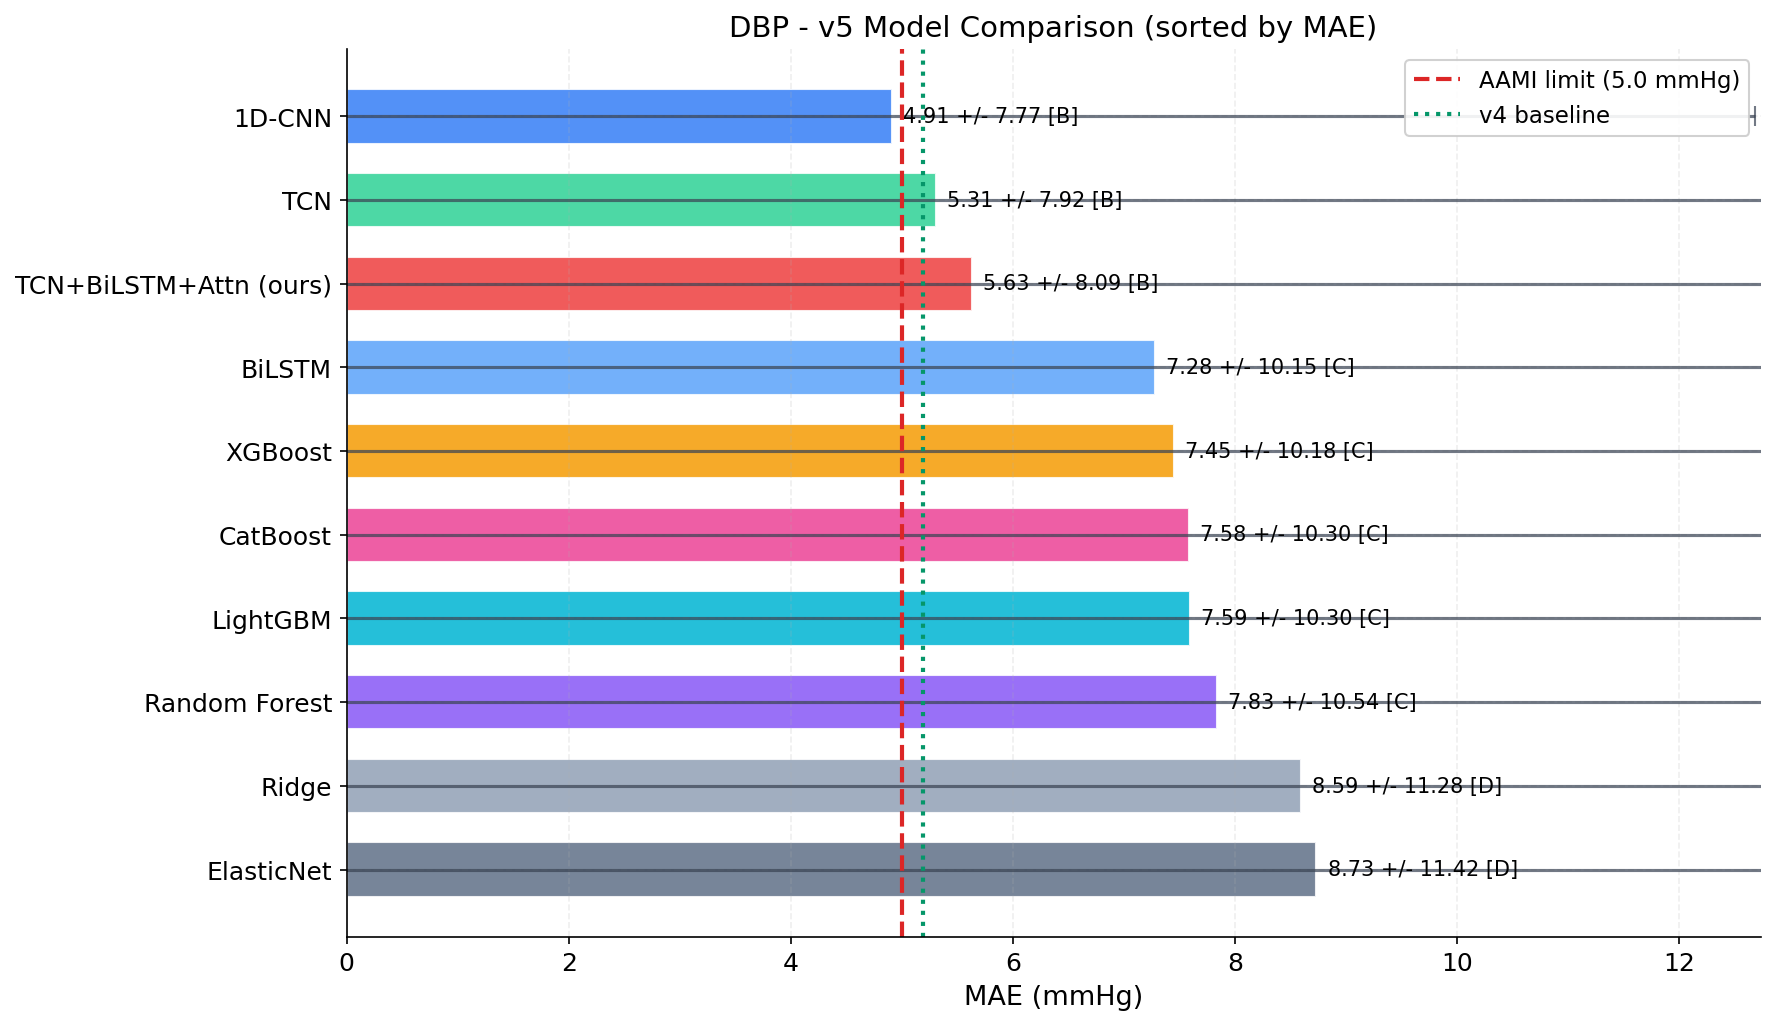
\includegraphics[width=\linewidth]{fig_13_mae_comparison_dbp.png}
\captionof{figure}{DBP MAE across all ten models; the best model clears the
AAMI limit for diastolic pressure.}
\label{fig:maedbp}
\end{minipage}
\end{figure}

\subsubsection{Clinical Evaluation of the Best Model}

The clinical-agreement figures for the best model (1D-CNN) are shown in
Figures~\ref{fig:scatter}--\ref{fig:perclass}. The scatter plots
(Figure~\ref{fig:scatter}) show true-versus-predicted values colored by absolute
error with $\pm$5\,mmHg reference bands; the Bland--Altman plots
(Figure~\ref{fig:bland})~\cite{blandaltman} show mean bias and 95\% limits of
agreement; and the per-class MAE breakdown (Figure~\ref{fig:perclass}) reveals
whether error is evenly spread or concentrated in the rarer BP categories that
sample weighting was designed to protect.

\begin{figure}[H]
\centering
\begin{minipage}{0.49\linewidth}\centering
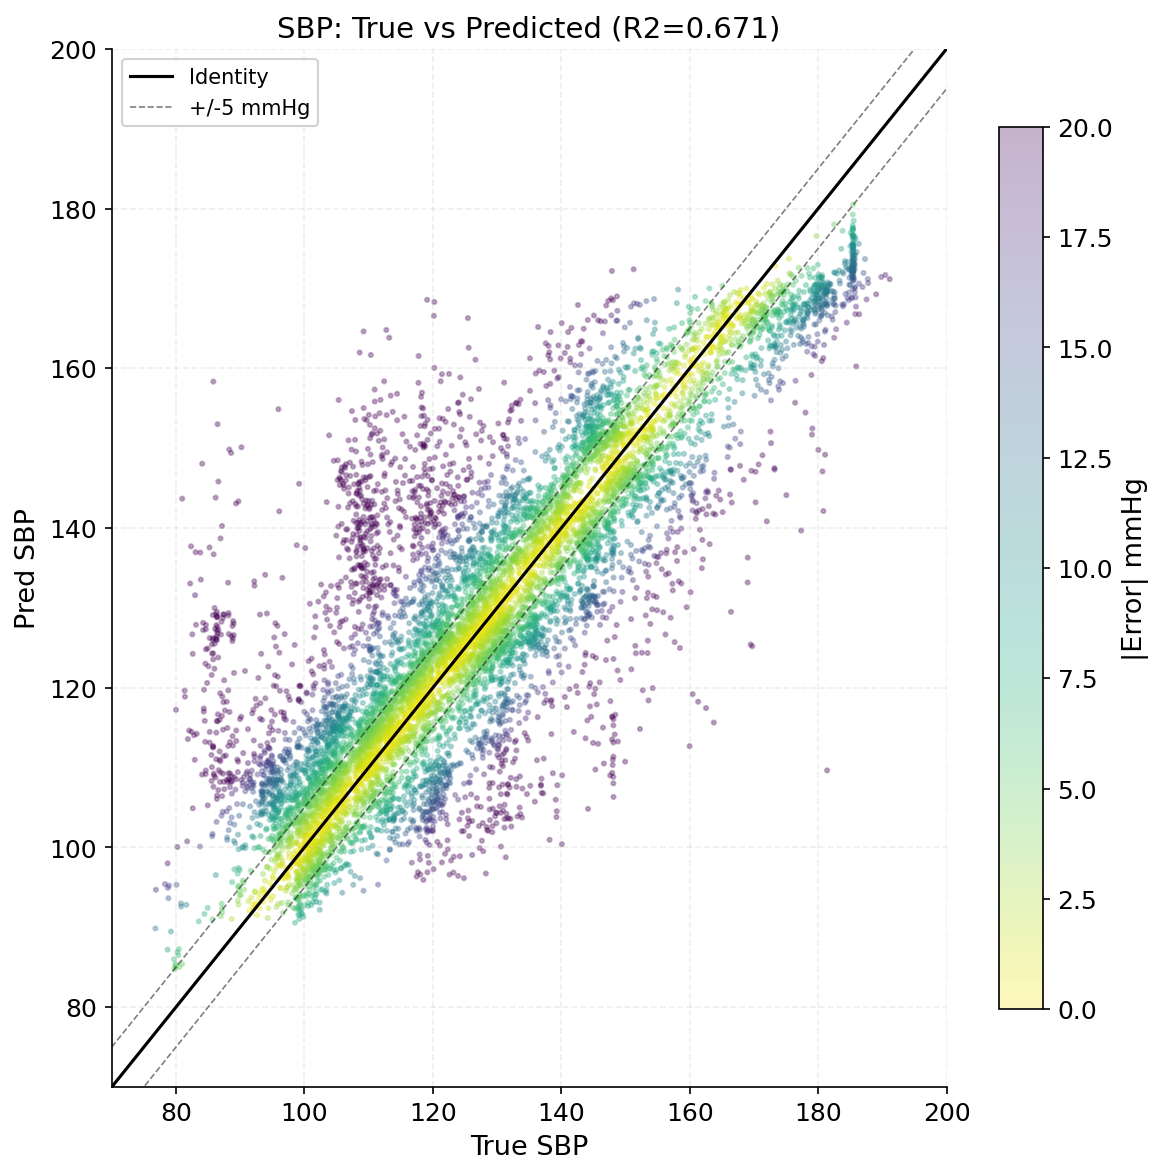
\includegraphics[width=\linewidth]{fig_17_scatter_sbp.png}\\[2pt]
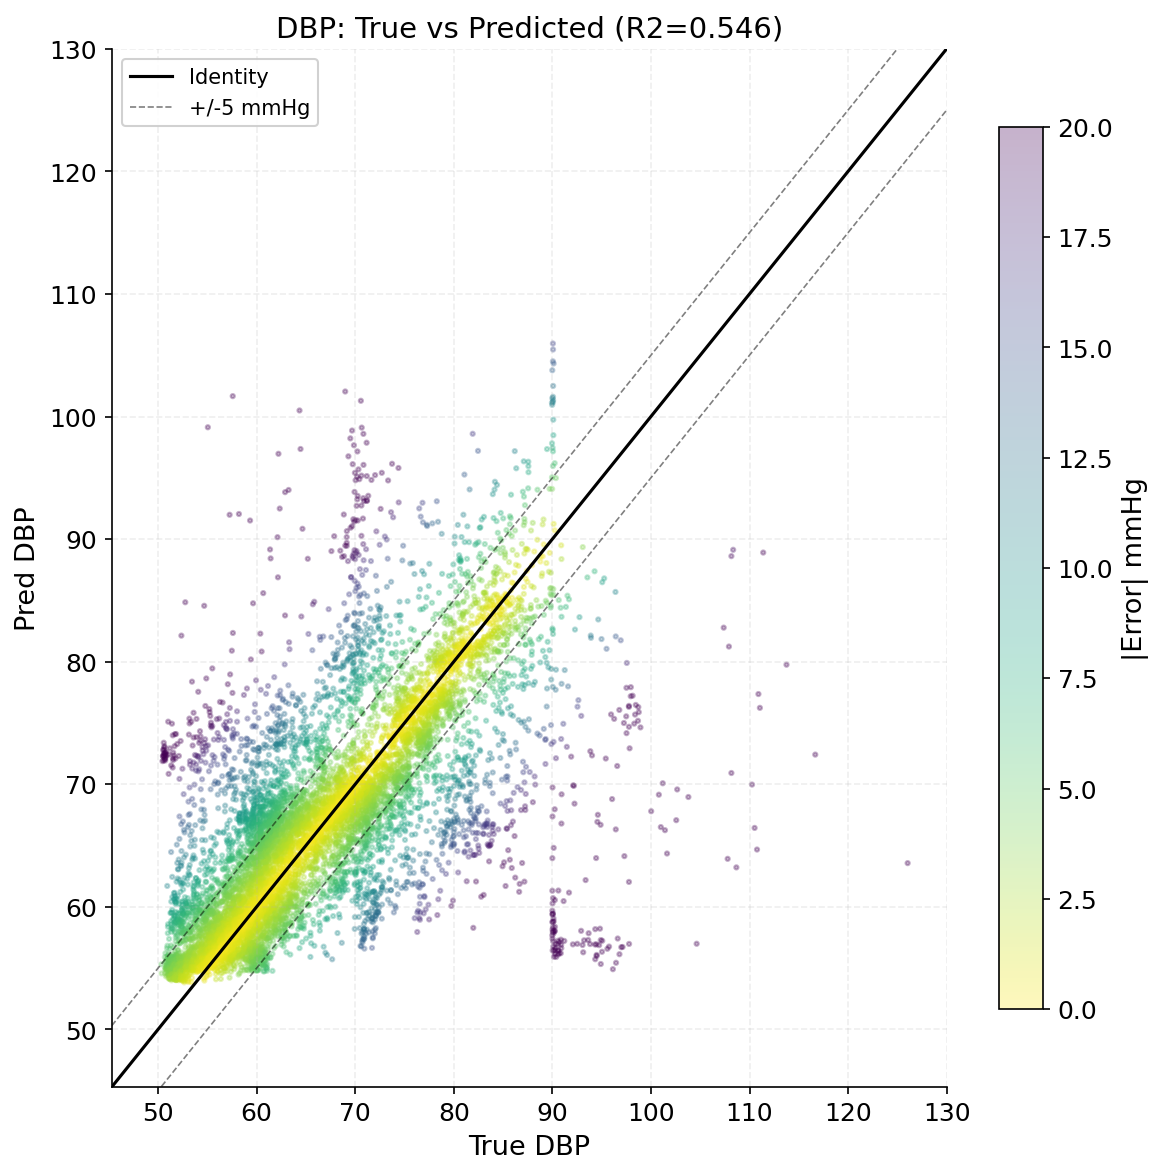
\includegraphics[width=\linewidth]{fig_18_scatter_dbp.png}
\captionof{figure}{True vs. predicted SBP (top) and DBP (bottom), colored by
absolute error.}
\label{fig:scatter}
\end{minipage}\hfill
\begin{minipage}{0.49\linewidth}\centering
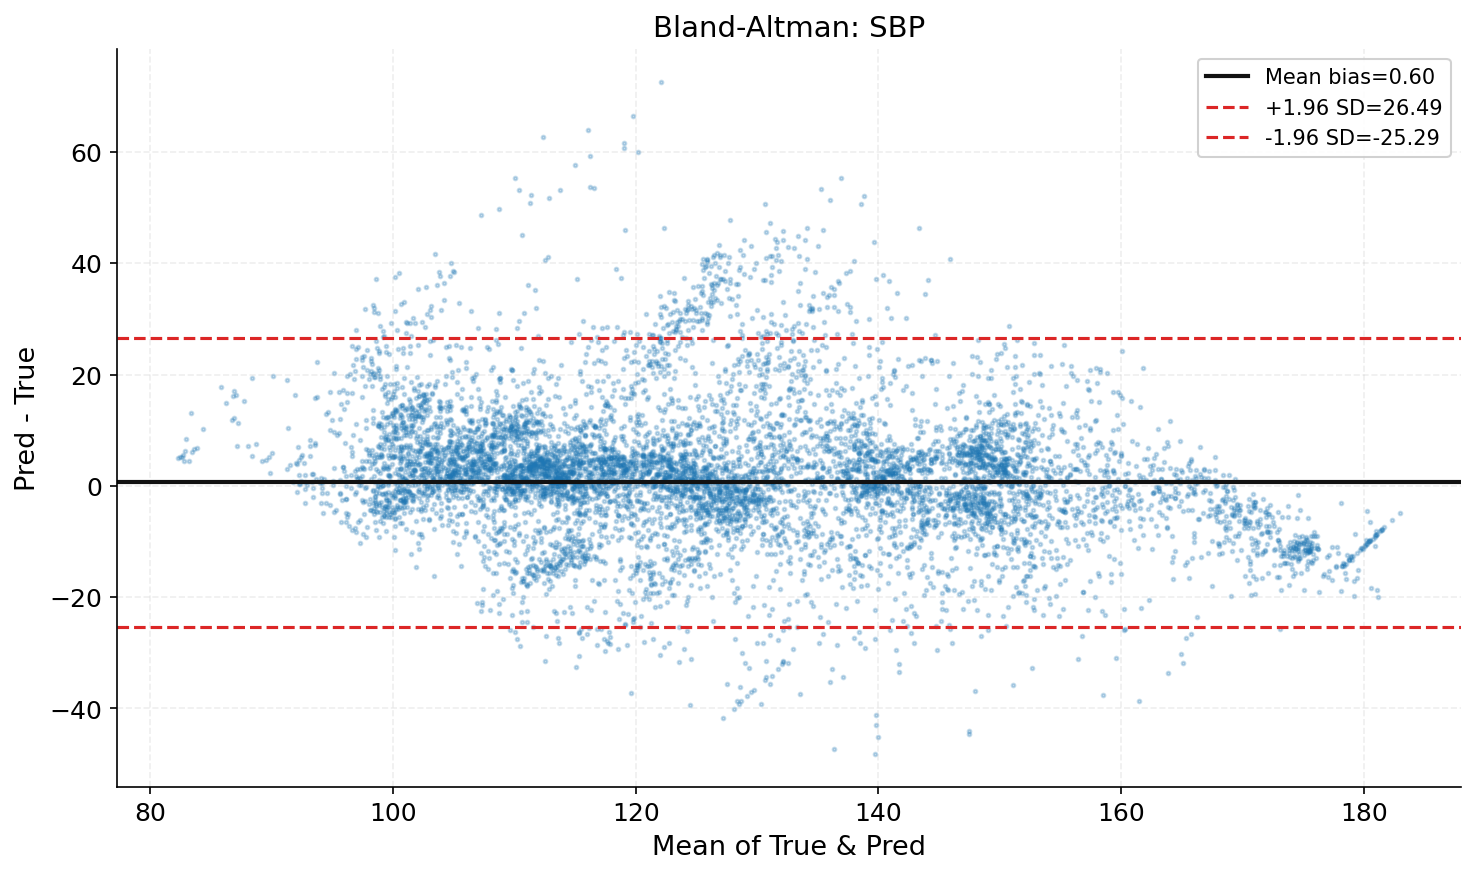
\includegraphics[width=\linewidth]{fig_20_bland_altman_sbp.png}\\[2pt]
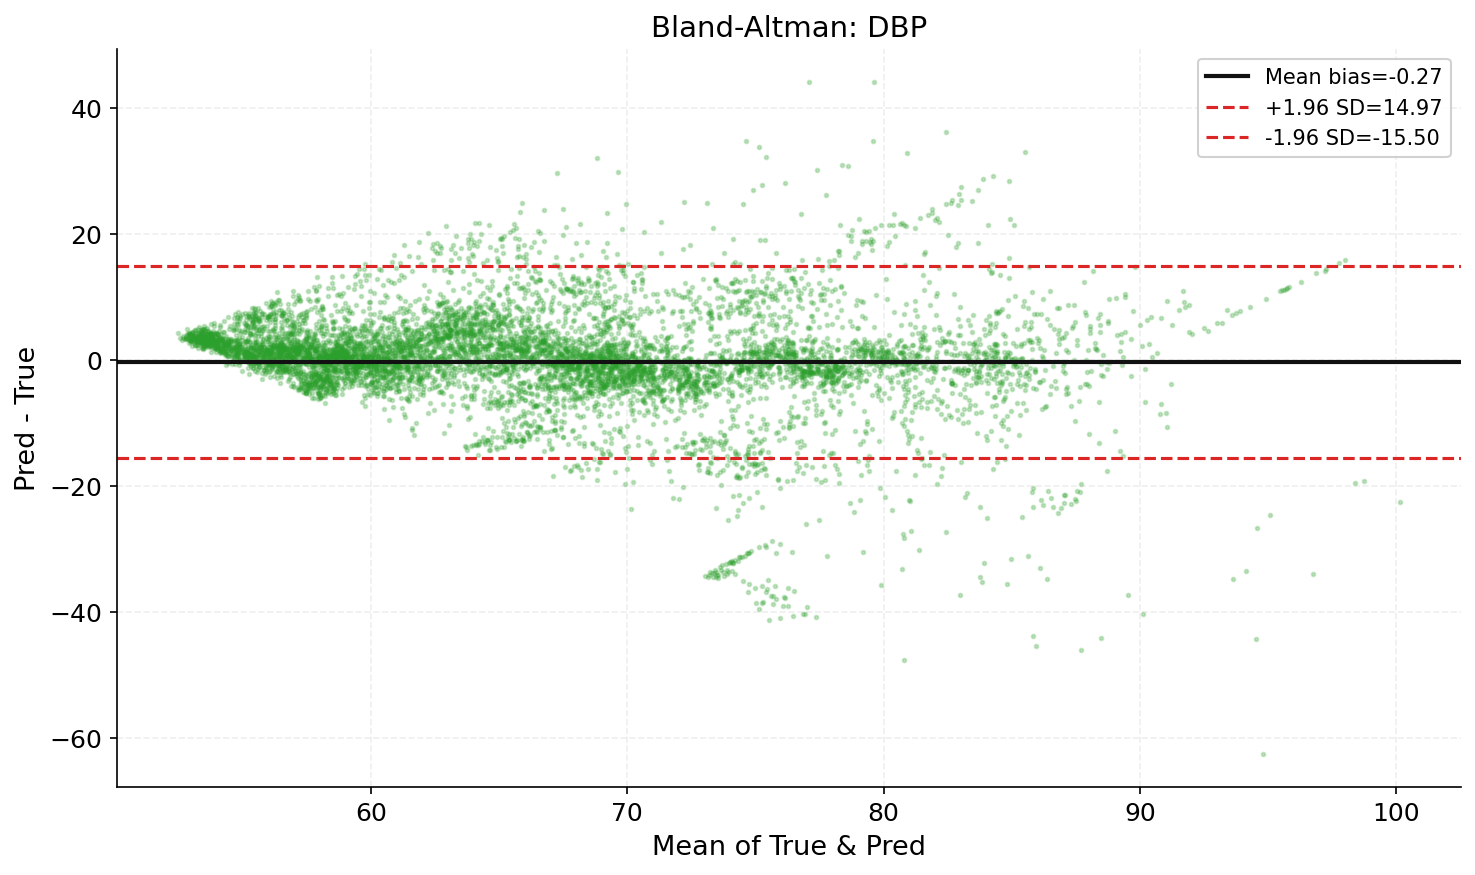
\includegraphics[width=\linewidth]{fig_21_bland_altman_dbp.png}
\captionof{figure}{Bland--Altman agreement for SBP (top) and DBP (bottom): mean
bias $\pm$ 1.96\,SD limits of agreement.}
\label{fig:bland}
\end{minipage}
\end{figure}

\begin{figure}[H]
\centering
\begin{minipage}{0.49\linewidth}\centering
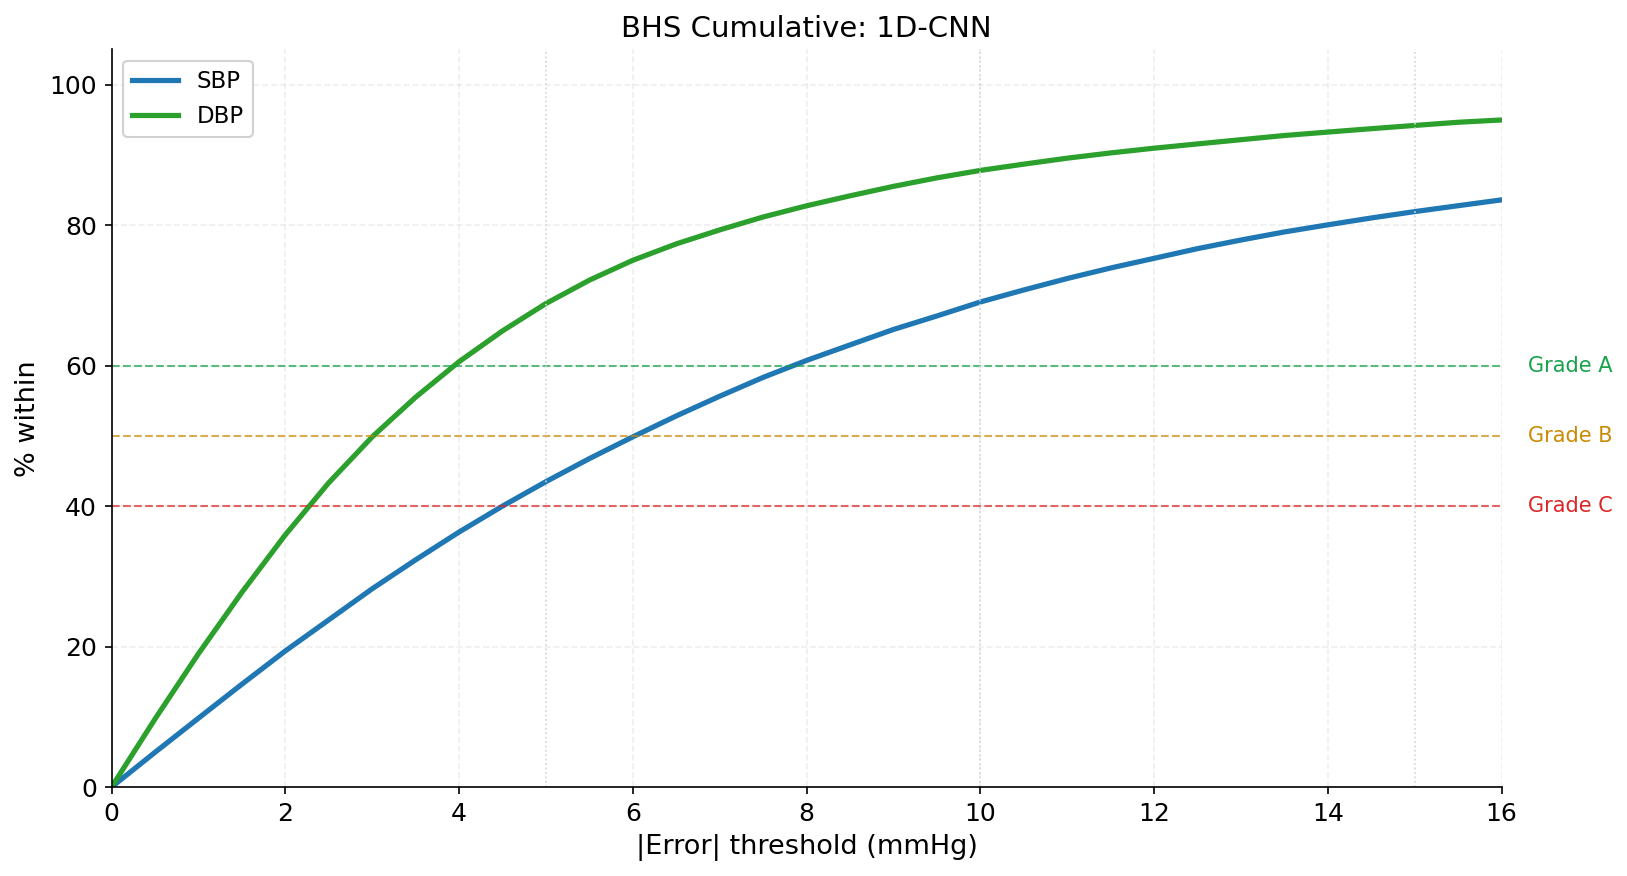
\includegraphics[width=\linewidth]{fig_23_bhs_best_model.png}
\captionof{figure}{Cumulative error-threshold curve for the best model against
the BHS A/B/C grade bands.}
\label{fig:bhs}
\end{minipage}\hfill
\begin{minipage}{0.49\linewidth}\centering
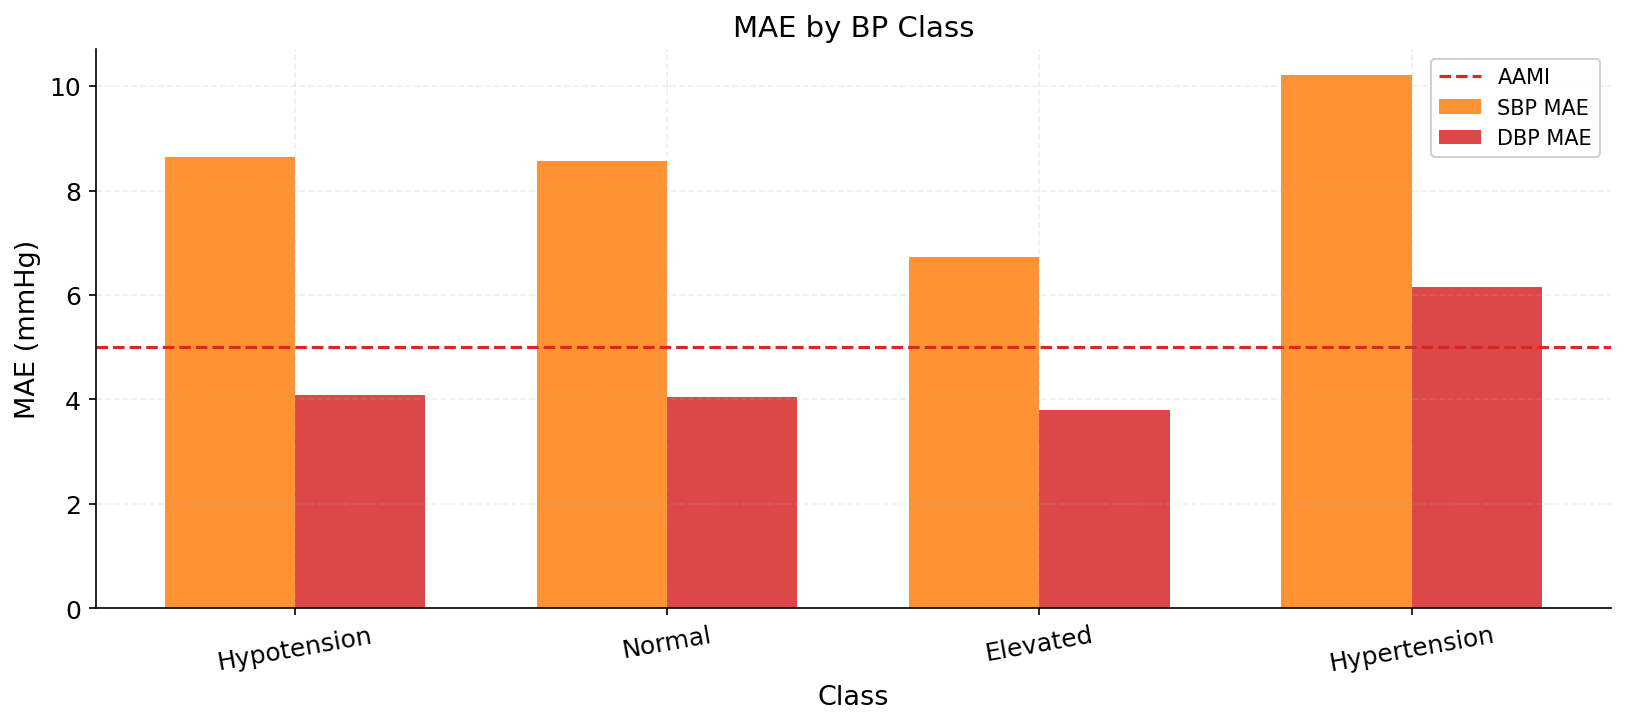
\includegraphics[width=\linewidth]{fig_24_per_class_mae.png}
\captionof{figure}{Per-class MAE across the four BP categories: error is not
uniform across the pooled AAMI/BHS headline.}
\label{fig:perclass}
\end{minipage}
\end{figure}

For context, the notebook tracks a ``v4 baseline'' (SBP MAE 9.13, DBP MAE 5.19)
from an earlier, larger, unregularized model. The current best model (SBP MAE
9.08) is a small improvement on SBP and a slightly larger one on DBP (4.91 vs.
5.19) --- modest gains achieved with better-controlled overfitting rather than a
fundamentally different result. Figure~\ref{fig:ablation} summarizes the
rationale behind the final ablation choices.

\begin{figure}[H]\centering
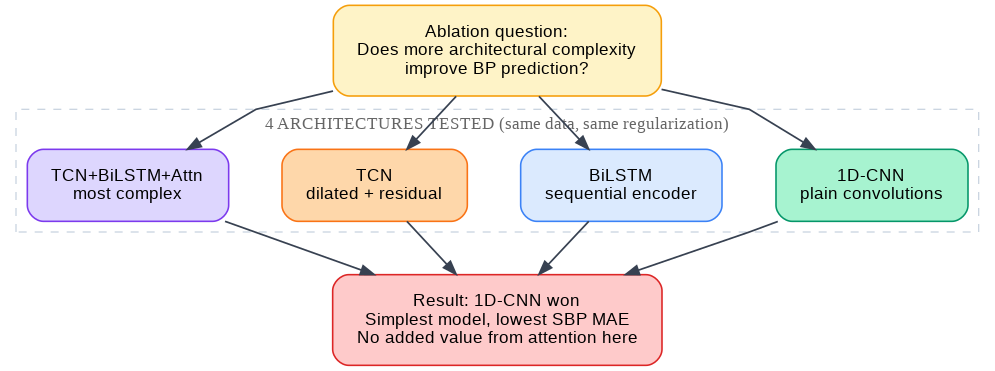
\includegraphics[width=0.8\linewidth]{fig_41_ablation_rationale.png}
\caption{Ablation rationale: how the final configuration was reached from the
earlier over-parameterized and over-balanced attempts.}
\label{fig:ablation}\end{figure}

\subsection{Symptom-Checker Results}
\label{sec:symresults}

From the model's own generated metadata and evaluation report:

\begin{itemize}[leftmargin=1.4em]
  \item \textbf{Top-1 accuracy: 0.8581}
  \item \textbf{Top-3 accuracy: 0.9549}
\end{itemize}

The report explicitly disowns an older 0.9034 accuracy figure sometimes quoted
for the v1 model as a fair comparison point, because that number was measured on
the same narrow synthetic method used to train it, with no held-out real-world
distribution.

\subsubsection{The Confusable-Pair Check Works}

The three-way Common Cold / Influenza / COVID-19 split and the Hypertension /
Migraine / Stroke split are both resolved with \emph{zero} cross-confusion in
the held-out test set --- the targeted differentiation strategy achieved exactly
what it set out to do.

\subsubsection{The Ten Worst Classes Are Cardiac}

The ten worst-performing classes are almost entirely cardiac subtypes
(Table~\ref{tab:worstclasses}). Because cardiovascular disease is the project's
core clinical focus, this is a meaningful, practically relevant weakness, not a
peripheral one: the model is weakest exactly where the product needs it to be
strong. These diseases share heavily overlapping symptom sets in the taxonomy
(fatigue, palpitations, chest pain, dyspnea, edema), and the synthetic
generator did not apply the same targeted differentiation to these cardiac pairs
that it applied to the respiratory and hypertension/neurological triads.

\begin{table}[H]
\centering
\caption{The ten lowest per-class top-1 accuracies --- almost all cardiac
subtypes.}
\label{tab:worstclasses}
\small
\begin{tabular}{@{}lr@{}}
\toprule
\textbf{Disease} & \textbf{Top-1 accuracy} \\
\midrule
Myocarditis & 0.350 \\
Hypertrophic cardiomyopathy & 0.400 \\
Coronary artery disease & 0.517 \\
Congestive heart failure & 0.600 \\
Pericarditis & 0.600 \\
Ventricular tachycardia & 0.650 \\
Heart failure & 0.683 \\
Pulmonary hypertension & 0.683 \\
Stable angina & 0.700 \\
Aortic stenosis & 0.750 \\
\bottomrule
\end{tabular}
\end{table}

\subsubsection{The Production Model Is Not the Best-Scoring Model}

A more fundamental, easy-to-miss finding: the baseline comparison
(Table~\ref{tab:baselines}), trained on the identical feature matrix and split,
shows plain Logistic Regression scoring \textbf{0.8703} and Random Forest
\textbf{0.8663} --- both higher than LightGBM's 0.8581. The model chosen for
production is not the one that scored highest on this exact dataset. This mirrors
the BP result, where the simplest deep-learning model also beat a more
sophisticated one, and is reported here with the same lack of spin.

\begin{table}[H]
\centering
\caption{Symptom-checker model comparison on the identical structured dataset.}
\label{tab:baselines}
\small
\begin{tabular}{@{}lrc@{}}
\toprule
\textbf{Model} & \textbf{Top-1 accuracy} & \textbf{Status} \\
\midrule
Logistic Regression & 0.8703 & baseline (for comparison) \\
Random Forest & 0.8663 & baseline (for comparison) \\
LightGBM & 0.8581 & \textbf{deployed to production} \\
\bottomrule
\end{tabular}
\end{table}

\section{Interpretation of Results}

Two of this project's clearest results do not flatter its own preferred
architectures, and both are reported here rather than adjusted after the fact.
First, greater model sophistication did not translate into better
blood-pressure accuracy: the combined TCN+BiLSTM+attention model underperformed
a plain 1D-CNN, most plausibly because an 8-second, fixed-length single window
does not have much long-range temporal structure for a bidirectional recurrent
layer or self-attention to exploit. Second, the same pattern recurs
independently in the symptom checker, where LightGBM was outperformed by a plain
Logistic Regression baseline on the identical feature set. Encountering this
pattern in two separate subsystems is itself the project's most transferable
lesson: architectural complexity must earn its place against a simple baseline
that is actually run, not assumed away.

Both the cardiac-subtype weakness (symptom checker) and the SBP AAMI shortfall
(BP model) point to the same underlying theme: the project's two hardest, most
clinically relevant sub-problems are exactly the areas where the current models
are weakest --- a substantive, not cosmetic, limitation of the current system.

\subsection*{Is ``Best Model'' the Same Claim as ``Clinically Acceptable''? }

It is worth being explicit about a distinction this document has used
throughout but not yet named directly, because it is exactly the kind of
question a careful reviewer should ask: the 1D-CNN is called the \emph{best}
blood-pressure model, and yet the same section states it \emph{fails} the
AAMI~SP10 standard~\cite{aami} for systolic pressure. Both statements are true
at once because they answer two different questions. ``Best'' is a
\emph{comparative} claim --- among the ten models actually trained and
evaluated on the identical test set, the 1D-CNN has the lowest SBP and DBP
error of all of them. ``Passes AAMI'' is an \emph{absolute} clinical-acceptance
threshold, unrelated to how the model compares to any alternative --- it asks
only whether the error is small enough (MAE~$\le$~5\,mmHg, SD~$\le$~8\,mmHg) for
a device to be considered clinically interchangeable with a reference
sphygmomanometer. A model can legitimately be the best of a field and still not
clear an absolute bar the entire field misses.

Given that framing, choosing the 1D-CNN as the production model is, in this
document's assessment, still the correct engineering decision, for three
concrete reasons rather than as a default: first, \emph{no} model in the
ten-model comparison passes AAMI for SBP, so discarding the 1D-CNN in favor of
any alternative would not produce a passing model either --- it would only
produce a \emph{worse} one on both SBP and DBP simultaneously; second, the same
model \emph{does} clear AAMI for DBP, so shipping it delivers one clinically
validated number and one indicative number, rather than two indicative
numbers; third, the system does not quietly present the failing number as if
it had passed --- SBP is treated as a trend indicator throughout this
documentation and the product's own safety design (physiological clamping,
per-patient calibration, and the \texttt{COMPLETED\_PENDING\_BP} state that
withholds an unconfirmed number rather than showing it) rather than as a
diagnostic-grade reading. What would genuinely be the wrong call is not
shipping this model --- it is shipping it \emph{while presenting SBP as if it
had met the same clinical bar as DBP}. This document deliberately does not do
that, in the abstract, in this chapter, or in the conclusions
(Chapter~\ref{sec:conclusion}), and that separation is the actual safeguard,
not the model's accuracy alone. The honest summary a reviewer should take away
is: the best available model was chosen, its one real shortfall is named
precisely rather than hidden, and the product treats that shortfall as a
constraint on how the number is used, not as a defect to be quietly rounded
away.

\section{Calibration Simulation}
\label{sec:calibration}

The notebook simulates a specific product decision: would per-patient linear
calibration actually help on this exact test set? The corresponding product code
already exists as a working implementation wired into the BP submission
endpoint, so the simulation is best read as a validation exercise for the
general idea rather than an approximation the product still has to catch up to.

\textbf{Method.} For every test-set patient with at least 4 windows, the first 3
windows (in time order) are treated as an oracle calibration set --- their true
BP values stand in for perfect cuff readings. A scale/offset is fit by least
squares from those 3 points and applied to that patient's remaining windows;
metrics are recomputed across all patients' remaining windows pooled together.

\textbf{Result.} As Table~\ref{tab:calibration} shows, calibration made
\emph{both} SBP and DBP \emph{worse}, and DBP specifically regressed from an
AAMI pass to a fail (Figure~\ref{fig:calib}).

\begin{table}[H]
\centering
\caption{Oracle calibration simulation: calibration degraded accuracy on this
test set.}
\label{tab:calibration}
\small
\begin{tabular}{@{}lrrrr@{}}
\toprule
\textbf{Metric} & \textbf{SBP raw} & \textbf{SBP cal.} & \textbf{DBP raw} & \textbf{DBP cal.} \\
\midrule
MAE (mmHg) & 9.04 & 14.52 & 4.89 & 6.99 \\
SD (mmHg) & 13.15 & 16.20 & 7.74 & 8.45 \\
AAMI & FAIL & FAIL & PASS & FAIL \\
BHS & D & D & B & C \\
\bottomrule
\end{tabular}
\end{table}

\begin{figure}[H]\centering
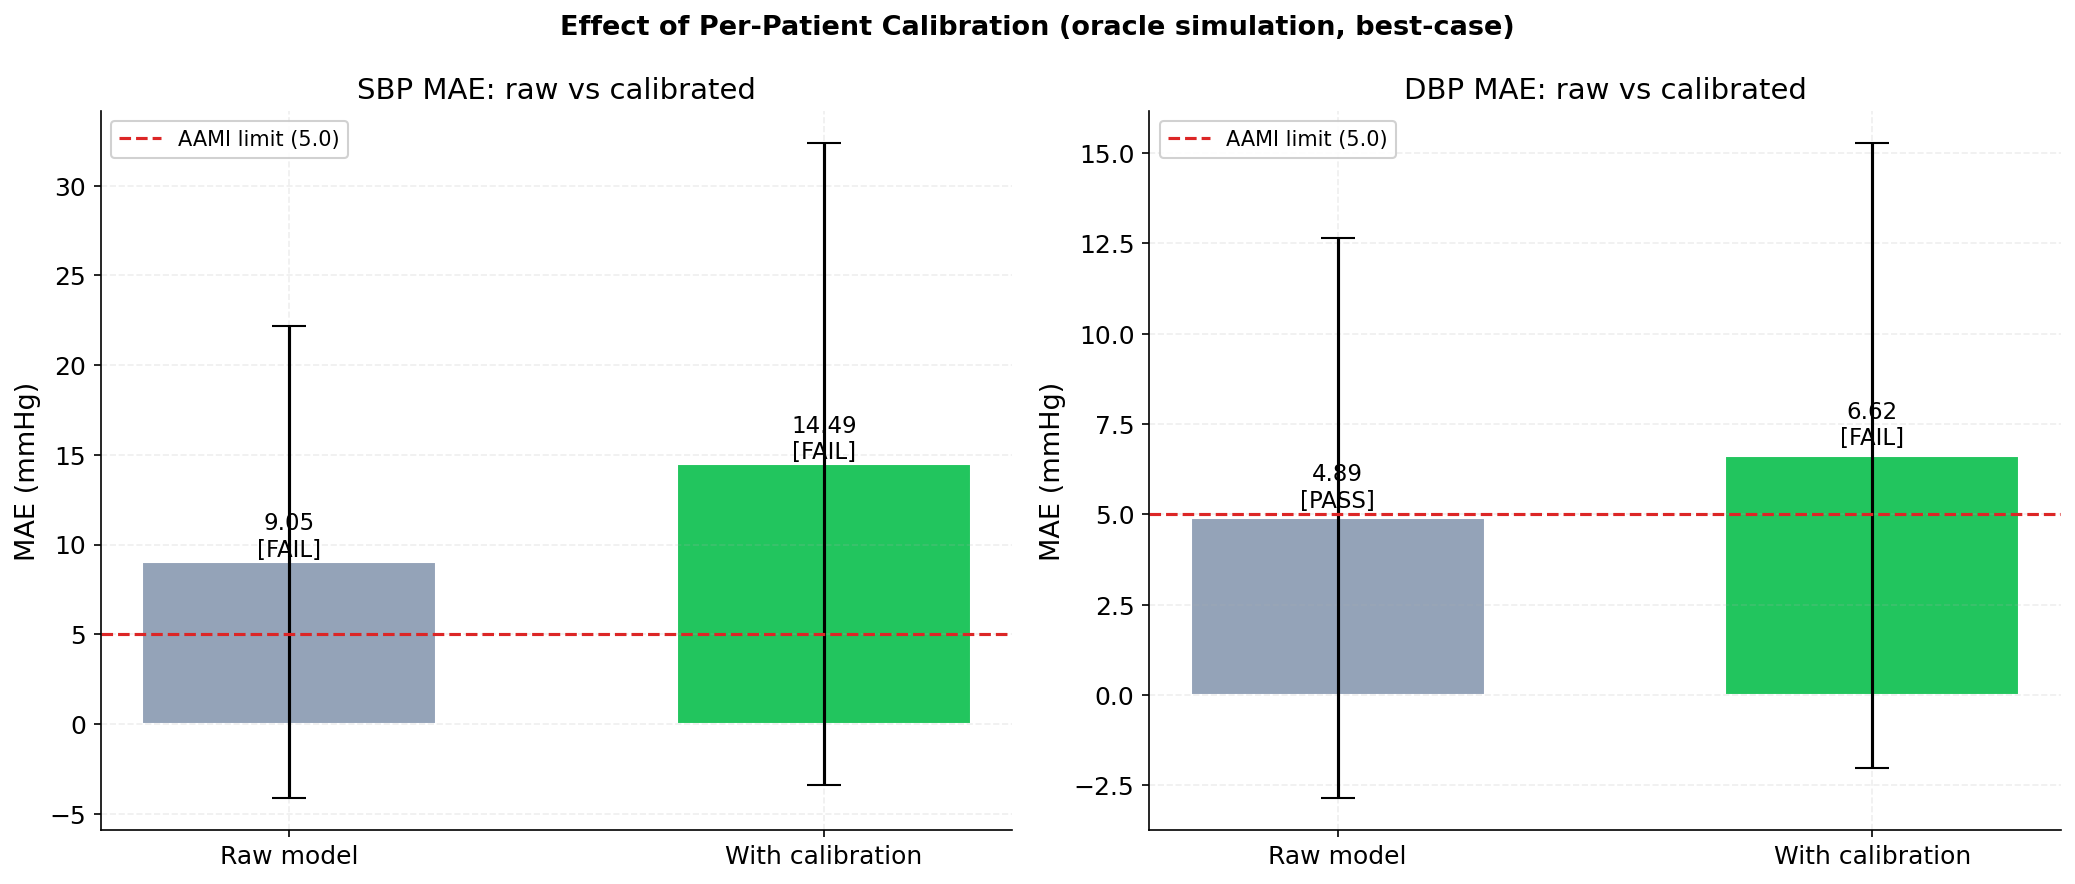
\includegraphics[width=0.85\linewidth]{fig_25_calibration_before_after.png}
\caption{Before/after the oracle calibration simulation. The negative result is
an artifact of the simulation's sampling, not a verdict on the deployed
service.}
\label{fig:calib}\end{figure}

The most likely explanation is how the calibration points were chosen: the three
``calibration'' windows are the first three 8-second, 50\%-overlapping windows
of a single continuous ICU recording, not three independent measurements at
meaningfully different times. The deployed calibration service accumulates its
samples the way the real product measures BP --- one submitted reading at a
time, over however many days it takes to reach its 8-sample linear-fit threshold
--- a fundamentally different sampling process. This project's interpretation is
therefore that the simulation does not faithfully represent the deployed service,
and its negative result should be read as evidence that the simulation's
methodology needs correcting, not as evidence against the calibration feature
itself, which remains unvalidated either way pending real, time-separated data.


%==============================================================================
\chapter{Illustrative Examples and Feature Flows}
%==============================================================================

This chapter traces the system's main features end to end through the actual
implementation, using sequence and state diagrams drawn directly from the code
paths they describe.

\section{Blood-Pressure Measurement Flow}

A complete guided measurement runs as follows. A scheduled reminder opens the
in-app measurement guide. The app polls live sensor status every two seconds
while the patient attaches the ECG leads and places a finger on the PPG sensor;
the firmware itself gates sample collection on both signals being present. Once
an 8-second, 800-sample window completes, it is uploaded to the backend, which
runs the model, applies the patient's current calibration (or withholds a plain,
uncalibrated number if calibration is not yet trustworthy), computes a risk
tier, persists the reading, and --- if the tier warrants --- sends a
rate-limited emergency push to every linked caregiver.
Figure~\ref{fig:bpseq} shows this as a sequence diagram.

\begin{figure}[H]
\centering
\resizebox{\linewidth}{!}{%
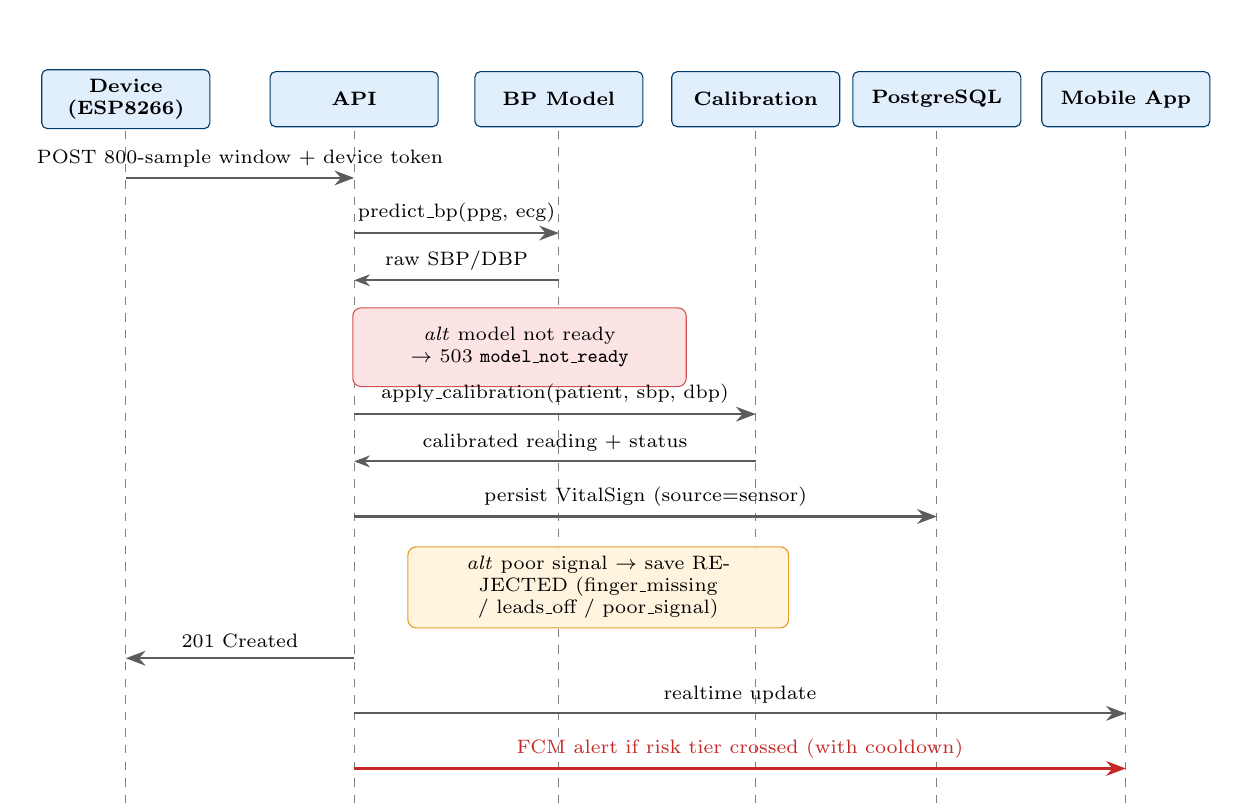
\begin{tikzpicture}[font=\scriptsize]
% Lifelines
\def\ytop{0} \def\ybot{-9.2}
\foreach \x/\name in {0/Device (ESP8266), 2.9/API, 5.5/BP Model, 8.0/Calibration, 10.3/PostgreSQL, 12.7/Mobile App}{
  \node[draw=primaryblue, fill=nodeblue, rounded corners=2pt, font=\scriptsize\bfseries,
        text width=1.9cm, align=center, minimum height=0.7cm] at (\x,\ytop) {\name};
  \draw[dashed, gray] (\x,-0.4) -- (\x,\ybot);
}
% Messages
\draw[flow] (0,-1.0) -- node[above,font=\scriptsize]{POST 800-sample window + device token} (2.9,-1.0);
\draw[flow] (2.9,-1.7) -- node[above,font=\scriptsize]{predict\_bp(ppg, ecg)} (5.5,-1.7);
\draw[{Stealth[length=2mm]}-, thick, draw=darkgray!80] (2.9,-2.3) -- node[above,font=\scriptsize]{raw SBP/DBP} (5.5,-2.3);
% not ready alt
\node[rbox, text width=4.0cm, font=\scriptsize] at (5.0,-3.15) (alt) {\textit{alt} model not ready $\rightarrow$ 503 \texttt{model\_not\_ready}};
\draw[flow] (2.9,-4.0) -- node[above,font=\scriptsize]{apply\_calibration(patient, sbp, dbp)} (8.0,-4.0);
\draw[{Stealth[length=2mm]}-, thick, draw=darkgray!80] (2.9,-4.6) -- node[above,font=\scriptsize]{calibrated reading + status} (8.0,-4.6);
\draw[flow] (2.9,-5.3) -- node[above,font=\scriptsize]{persist VitalSign (source=sensor)} (10.3,-5.3);
% poor signal alt
\node[abox, text width=4.6cm, font=\scriptsize] at (6.0,-6.2) {\textit{alt} poor signal $\rightarrow$ save REJECTED (finger\_missing / leads\_off / poor\_signal)};
\draw[flow] (2.9,-7.1) -- node[above,font=\scriptsize]{201 Created} (0,-7.1);
\draw[flow] (2.9,-7.8) -- node[above,font=\scriptsize]{realtime update} (12.7,-7.8);
\draw[flow, draw=softred] (2.9,-8.5) -- node[above,font=\scriptsize,text=softred]{FCM alert if risk tier crossed (with cooldown)} (12.7,-8.5);
\end{tikzpicture}
}%
\caption{Blood-pressure measurement sequence, from the device window upload
through model inference, calibration, persistence, and conditional alerting.}
\label{fig:bpseq}
\end{figure}

\subsection{The Post-Inference State Machine}

The part a patient actually experiences is a real state machine, not just ``save
it and show it'' (Figure~\ref{fig:bpstate}). The \texttt{COMPLETED\_PENDING\_BP}
state is the detail most easily missed: until a patient has enough calibration
history for the fit to be trusted (8+ paired samples, or at least a non-stale,
non-clamped fit), the backend deliberately withholds the numeric SBP/DBP and
requires a manual cuff confirmation to close the loop --- which is also how new
calibration samples are collected in the first place.

\begin{figure}[H]
\centering
\resizebox{\linewidth}{!}{%
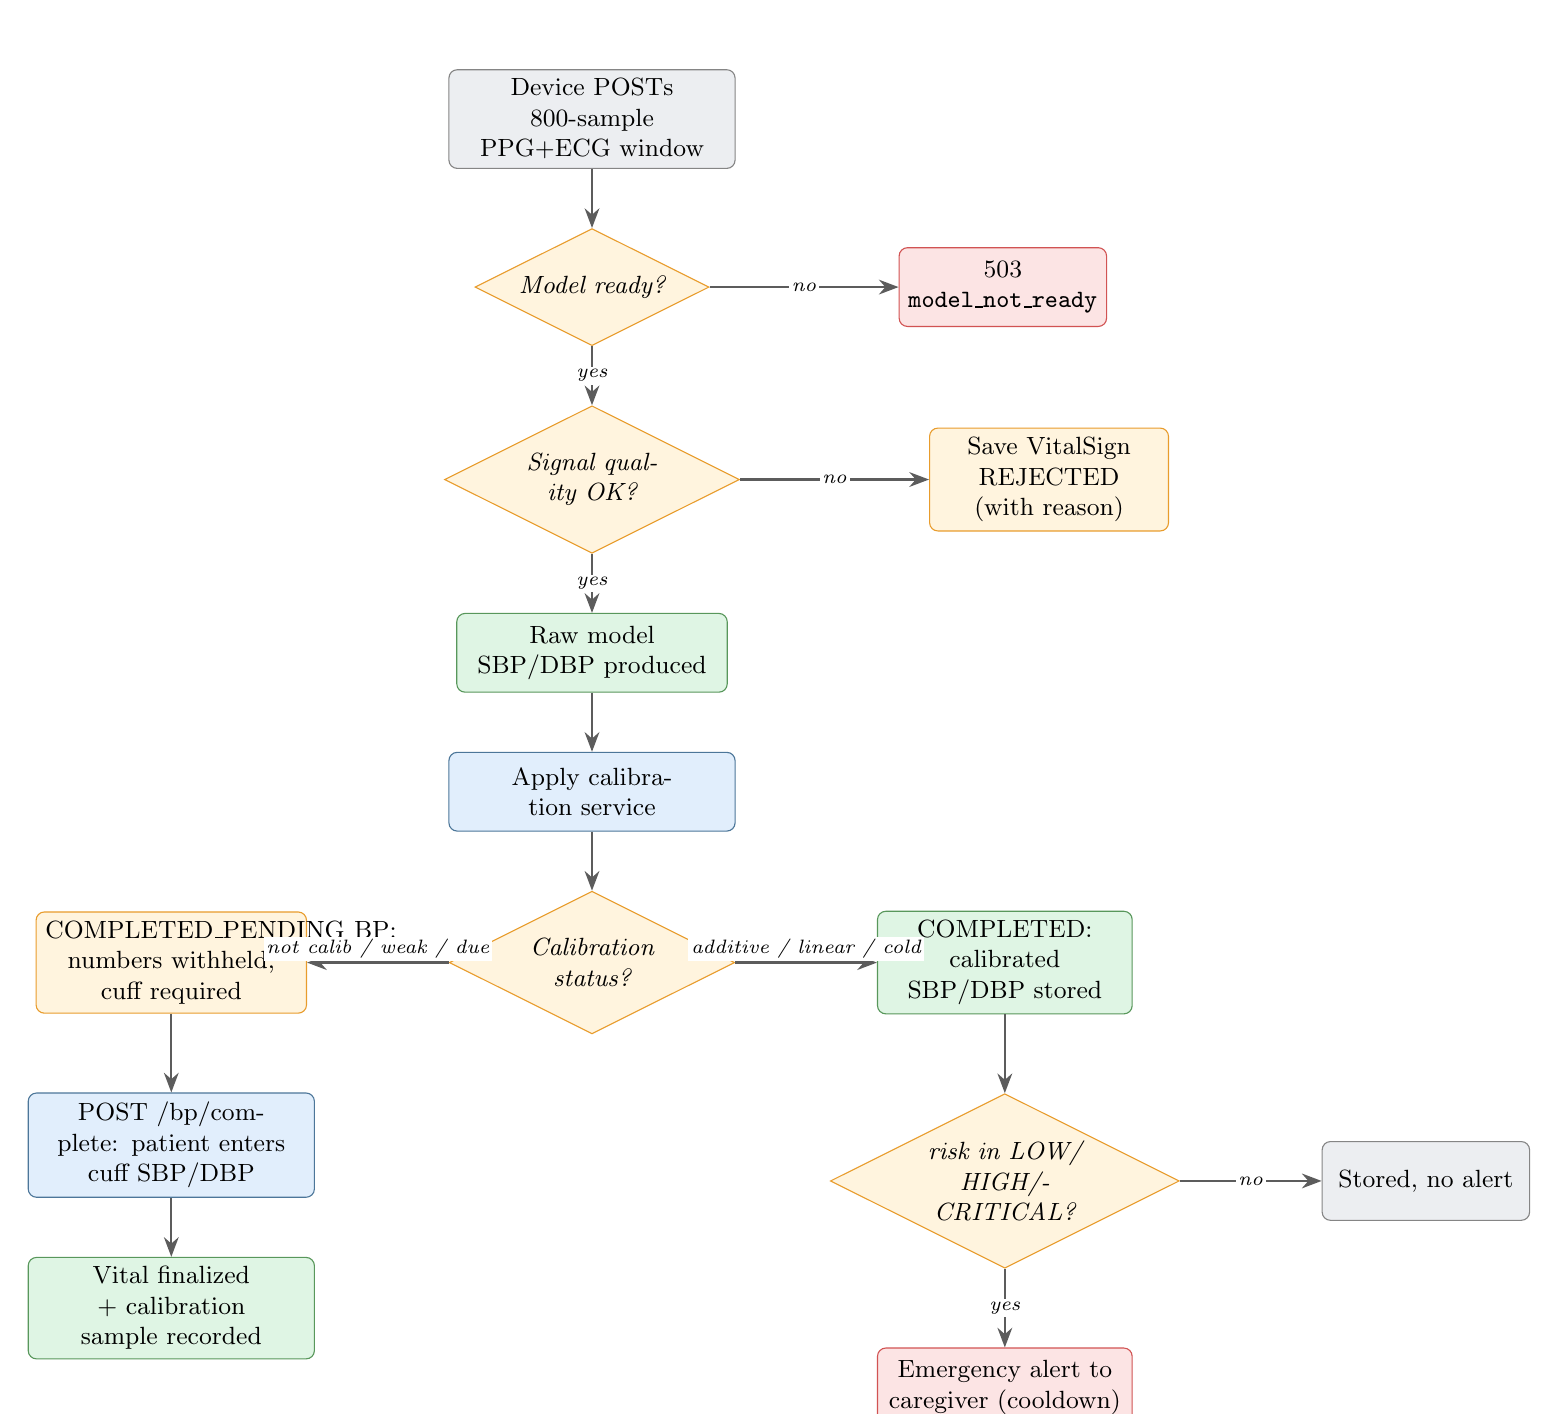
\begin{tikzpicture}[font=\scriptsize, node distance=0.75cm and 0.9cm]
\node[graybox, text width=3.4cm] (a) {Device POSTs 800-sample PPG+ECG window};
\node[dec, below=of a] (b) {Model ready?};
\node[rbox, right=2.4cm of b, text width=2.4cm] (b1) {503 \texttt{model\_not\_ready}};
\node[dec, below=of b] (c) {Signal quality OK?};
\node[abox, right=2.4cm of c, text width=2.8cm] (d) {Save VitalSign REJECTED (with reason)};
\node[gbox, below=of c, text width=3.2cm] (e) {Raw model SBP/DBP produced};
\node[box, below=of e, text width=3.4cm] (f) {Apply calibration service};
\node[dec, below=of f] (g) {Calibration status?};
\node[abox, left=1.8cm of g, text width=3.2cm] (h) {COMPLETED\_PENDING\_BP: numbers withheld, cuff required};
\node[gbox, right=1.8cm of g, text width=3.0cm] (i) {COMPLETED: calibrated SBP/DBP stored};
\node[box, below=1.0cm of h, text width=3.4cm] (j) {POST /bp/complete: patient enters cuff SBP/DBP};
\node[gbox, below=of j, text width=3.4cm] (k) {Vital finalized + calibration sample recorded};
\node[dec, below=1.0cm of i] (l) {risk in LOW/ HIGH/CRITICAL?};
\node[rbox, below=1.0cm of l, text width=3.0cm] (m) {Emergency alert to caregiver (cooldown)};
\node[graybox, right=1.8cm of l, text width=2.4cm] (n) {Stored, no alert};

\draw[flow] (a) -- (b);
\draw[flow] (b) -- node[lbl]{no} (b1);
\draw[flow] (b) -- node[lbl]{yes} (c);
\draw[flow] (c) -- node[lbl]{no} (d);
\draw[flow] (c) -- node[lbl]{yes} (e);
\draw[flow] (e) -- (f);
\draw[flow] (f) -- (g);
\draw[flow] (g) -- node[lbl,above]{not calib / weak / due} (h);
\draw[flow] (g) -- node[lbl,above]{additive / linear / cold} (i);
\draw[flow] (h) -- (j);
\draw[flow] (j) -- (k);
\draw[flow] (i) -- (l);
\draw[flow] (l) -- node[lbl]{yes} (m);
\draw[flow] (l) -- node[lbl]{no} (n);
\end{tikzpicture}
}%
\caption{The blood-pressure submission state machine, traced from the submission
endpoint. The pending-BP branch is what generates the paired samples the
calibration fit later depends on.}
\label{fig:bpstate}
\end{figure}

\section{Calibration and Drift Decision Flow}

The calibration service fits $\mathit{adjusted} = \mathit{scale} \times
\mathit{model\_output} + \mathit{offset}$ per patient, upgrading its own fit
quality as more samples accumulate, and a separate scheduled job watches for
drift (Figure~\ref{fig:calibflow}). Under 8 paired samples it uses a robust
median-only additive offset; at 8 or more it upgrades to a least-squares linear
fit. Both paths clamp scale to $[0.70, 1.30]$ and offset to $[-25, +25]$\,mmHg.

\begin{figure}[H]
\centering
\resizebox{\linewidth}{!}{%
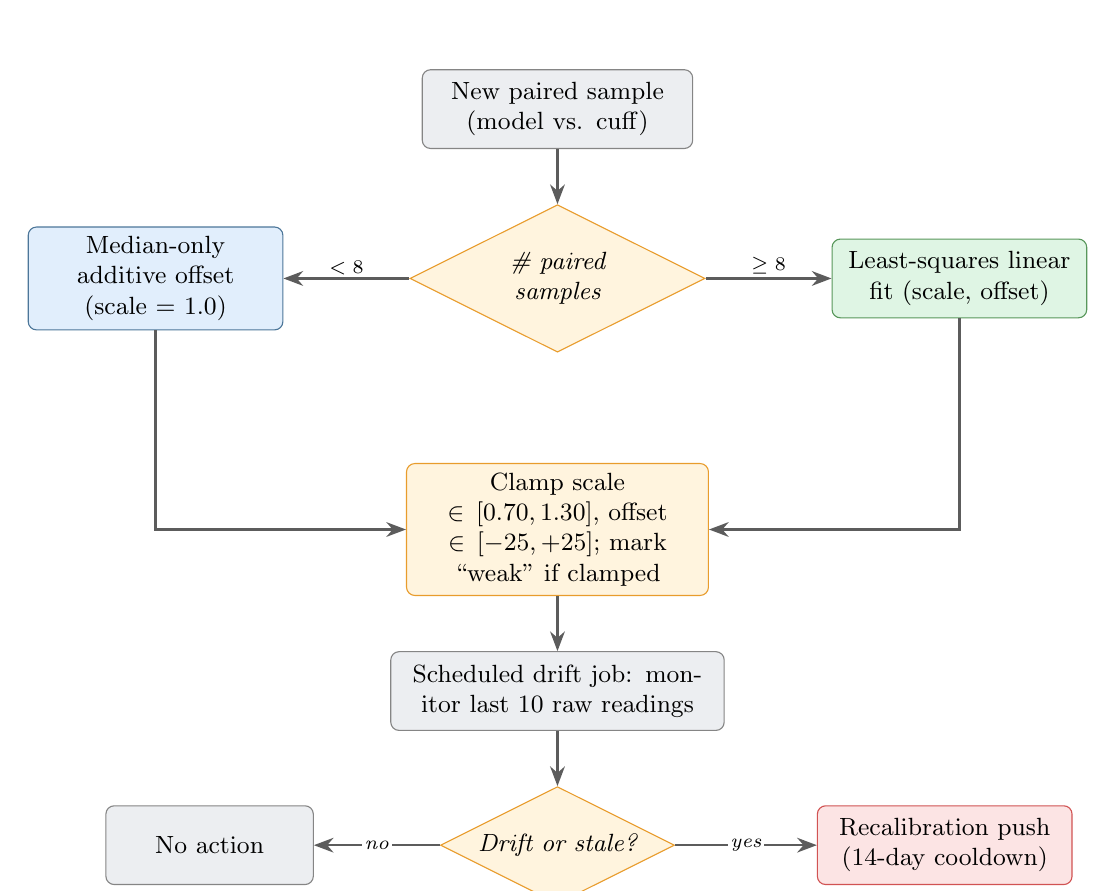
\begin{tikzpicture}[font=\scriptsize, node distance=0.7cm and 1.1cm]
\node[graybox, text width=3.2cm] (s) {New paired sample (model vs. cuff)};
\node[dec, below=of s] (n) {\# paired samples};
\node[box, left=1.6cm of n, text width=3.0cm] (med) {Median-only additive offset (scale = 1.0)};
\node[gbox, right=1.6cm of n, text width=3.0cm] (lin) {Least-squares linear fit (scale, offset)};
\node[abox, below=1.4cm of n, text width=3.6cm] (clamp) {Clamp scale $\in[0.70,1.30]$, offset $\in[-25,+25]$; mark ``weak'' if clamped};
\node[graybox, below=of clamp, text width=4.0cm] (drift) {Scheduled drift job: monitor last 10 raw readings};
\node[dec, below=of drift] (dd) {Drift or stale?};
\node[rbox, right=1.8cm of dd, text width=3.0cm] (notify) {Recalibration push (14-day cooldown)};
\node[graybox, left=1.6cm of dd, text width=2.4cm] (ok) {No action};

\draw[flow] (s) -- (n);
\draw[flow] (n) -- node[lbl,above]{$<8$} (med);
\draw[flow] (n) -- node[lbl,above]{$\ge 8$} (lin);
\draw[flow] (med) |- (clamp);
\draw[flow] (lin) |- (clamp);
\draw[flow] (clamp) -- (drift);
\draw[flow] (drift) -- (dd);
\draw[flow] (dd) -- node[lbl]{yes} (notify);
\draw[flow] (dd) -- node[lbl]{no} (ok);
\end{tikzpicture}
}%
\caption{Per-patient calibration fit and the scheduled drift/staleness job.
Drift is flagged on a sustained shift $>$8\,mmHg (SBP) or $>$5\,mmHg (DBP) from
baseline, or after 90 days.}
\label{fig:calibflow}
\end{figure}

\section{Medication Reminder Flow}

When a medication alarm fires, the scheduler collects the drawers assigned to
medications due at that time, optionally activates the smart box, and sends a
notification (Figure~\ref{fig:medseq}). This call is deliberately fail-soft: an
unreachable medicine box is logged and swallowed, never raised, so the alarm job
always completes and the patient still gets the phone notification even if the
physical box never lights up.

\begin{figure}[H]
\centering
\resizebox{\linewidth}{!}{%
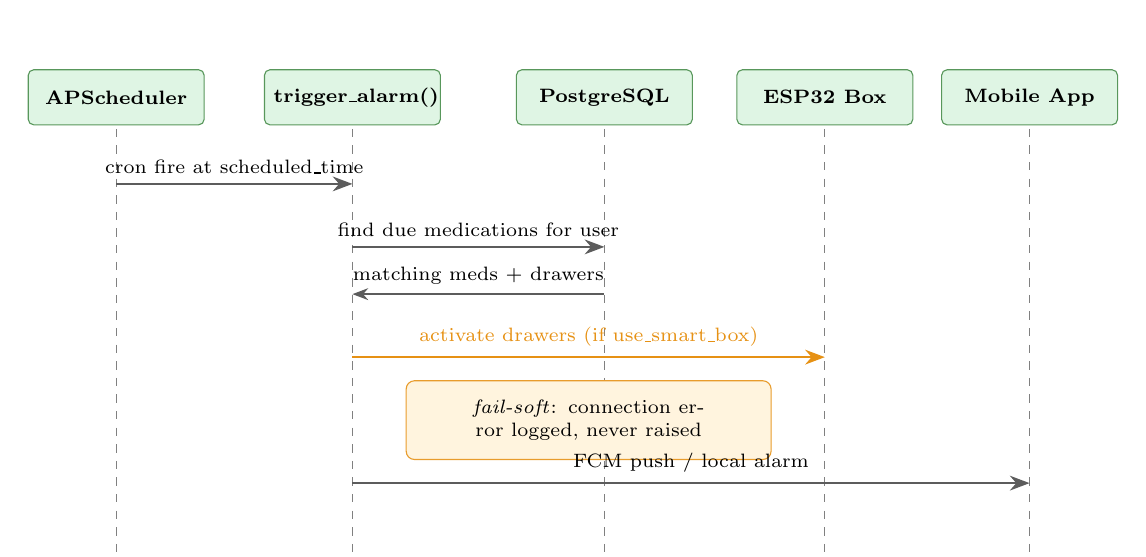
\begin{tikzpicture}[font=\scriptsize]
\def\ybot{-6.0}
\foreach \x/\name in {0/APScheduler, 3.0/trigger\_alarm(), 6.2/PostgreSQL, 9.0/ESP32 Box, 11.6/Mobile App}{
  \node[draw=softgreen!80, fill=nodegreen, rounded corners=2pt, font=\scriptsize\bfseries,
        text width=2.0cm, align=center, minimum height=0.7cm] at (\x,0) {\name};
  \draw[dashed, gray] (\x,-0.4) -- (\x,\ybot);
}
\draw[flow] (0,-1.1) -- node[above,font=\scriptsize]{cron fire at scheduled\_time} (3.0,-1.1);
\draw[flow] (3.0,-1.9) -- node[above,font=\scriptsize]{find due medications for user} (6.2,-1.9);
\draw[{Stealth[length=2mm]}-, thick, draw=darkgray!80] (3.0,-2.5) -- node[above,font=\scriptsize]{matching meds + drawers} (6.2,-2.5);
\draw[flow, draw=softamber] (3.0,-3.3) -- node[above,font=\scriptsize,text=softamber]{activate drawers (if use\_smart\_box)} (9.0,-3.3);
\node[abox, text width=4.4cm, font=\scriptsize] at (6.0,-4.1) {\textit{fail-soft}: connection error logged, never raised};
\draw[flow] (3.0,-4.9) -- node[above,font=\scriptsize]{FCM push / local alarm} (11.6,-4.9);
\end{tikzpicture}
}%
\caption{Medication reminder sequence: the smart-box activation is fail-soft, so
the phone notification is delivered regardless of hardware reachability.}
\label{fig:medseq}
\end{figure}

The complete decision tree --- single vs. grouped alarms, the smart-box check,
and the user's ``taken / snooze'' response --- is shown in
Figure~\ref{fig:alarmtree}.

\begin{figure}[H]\centering
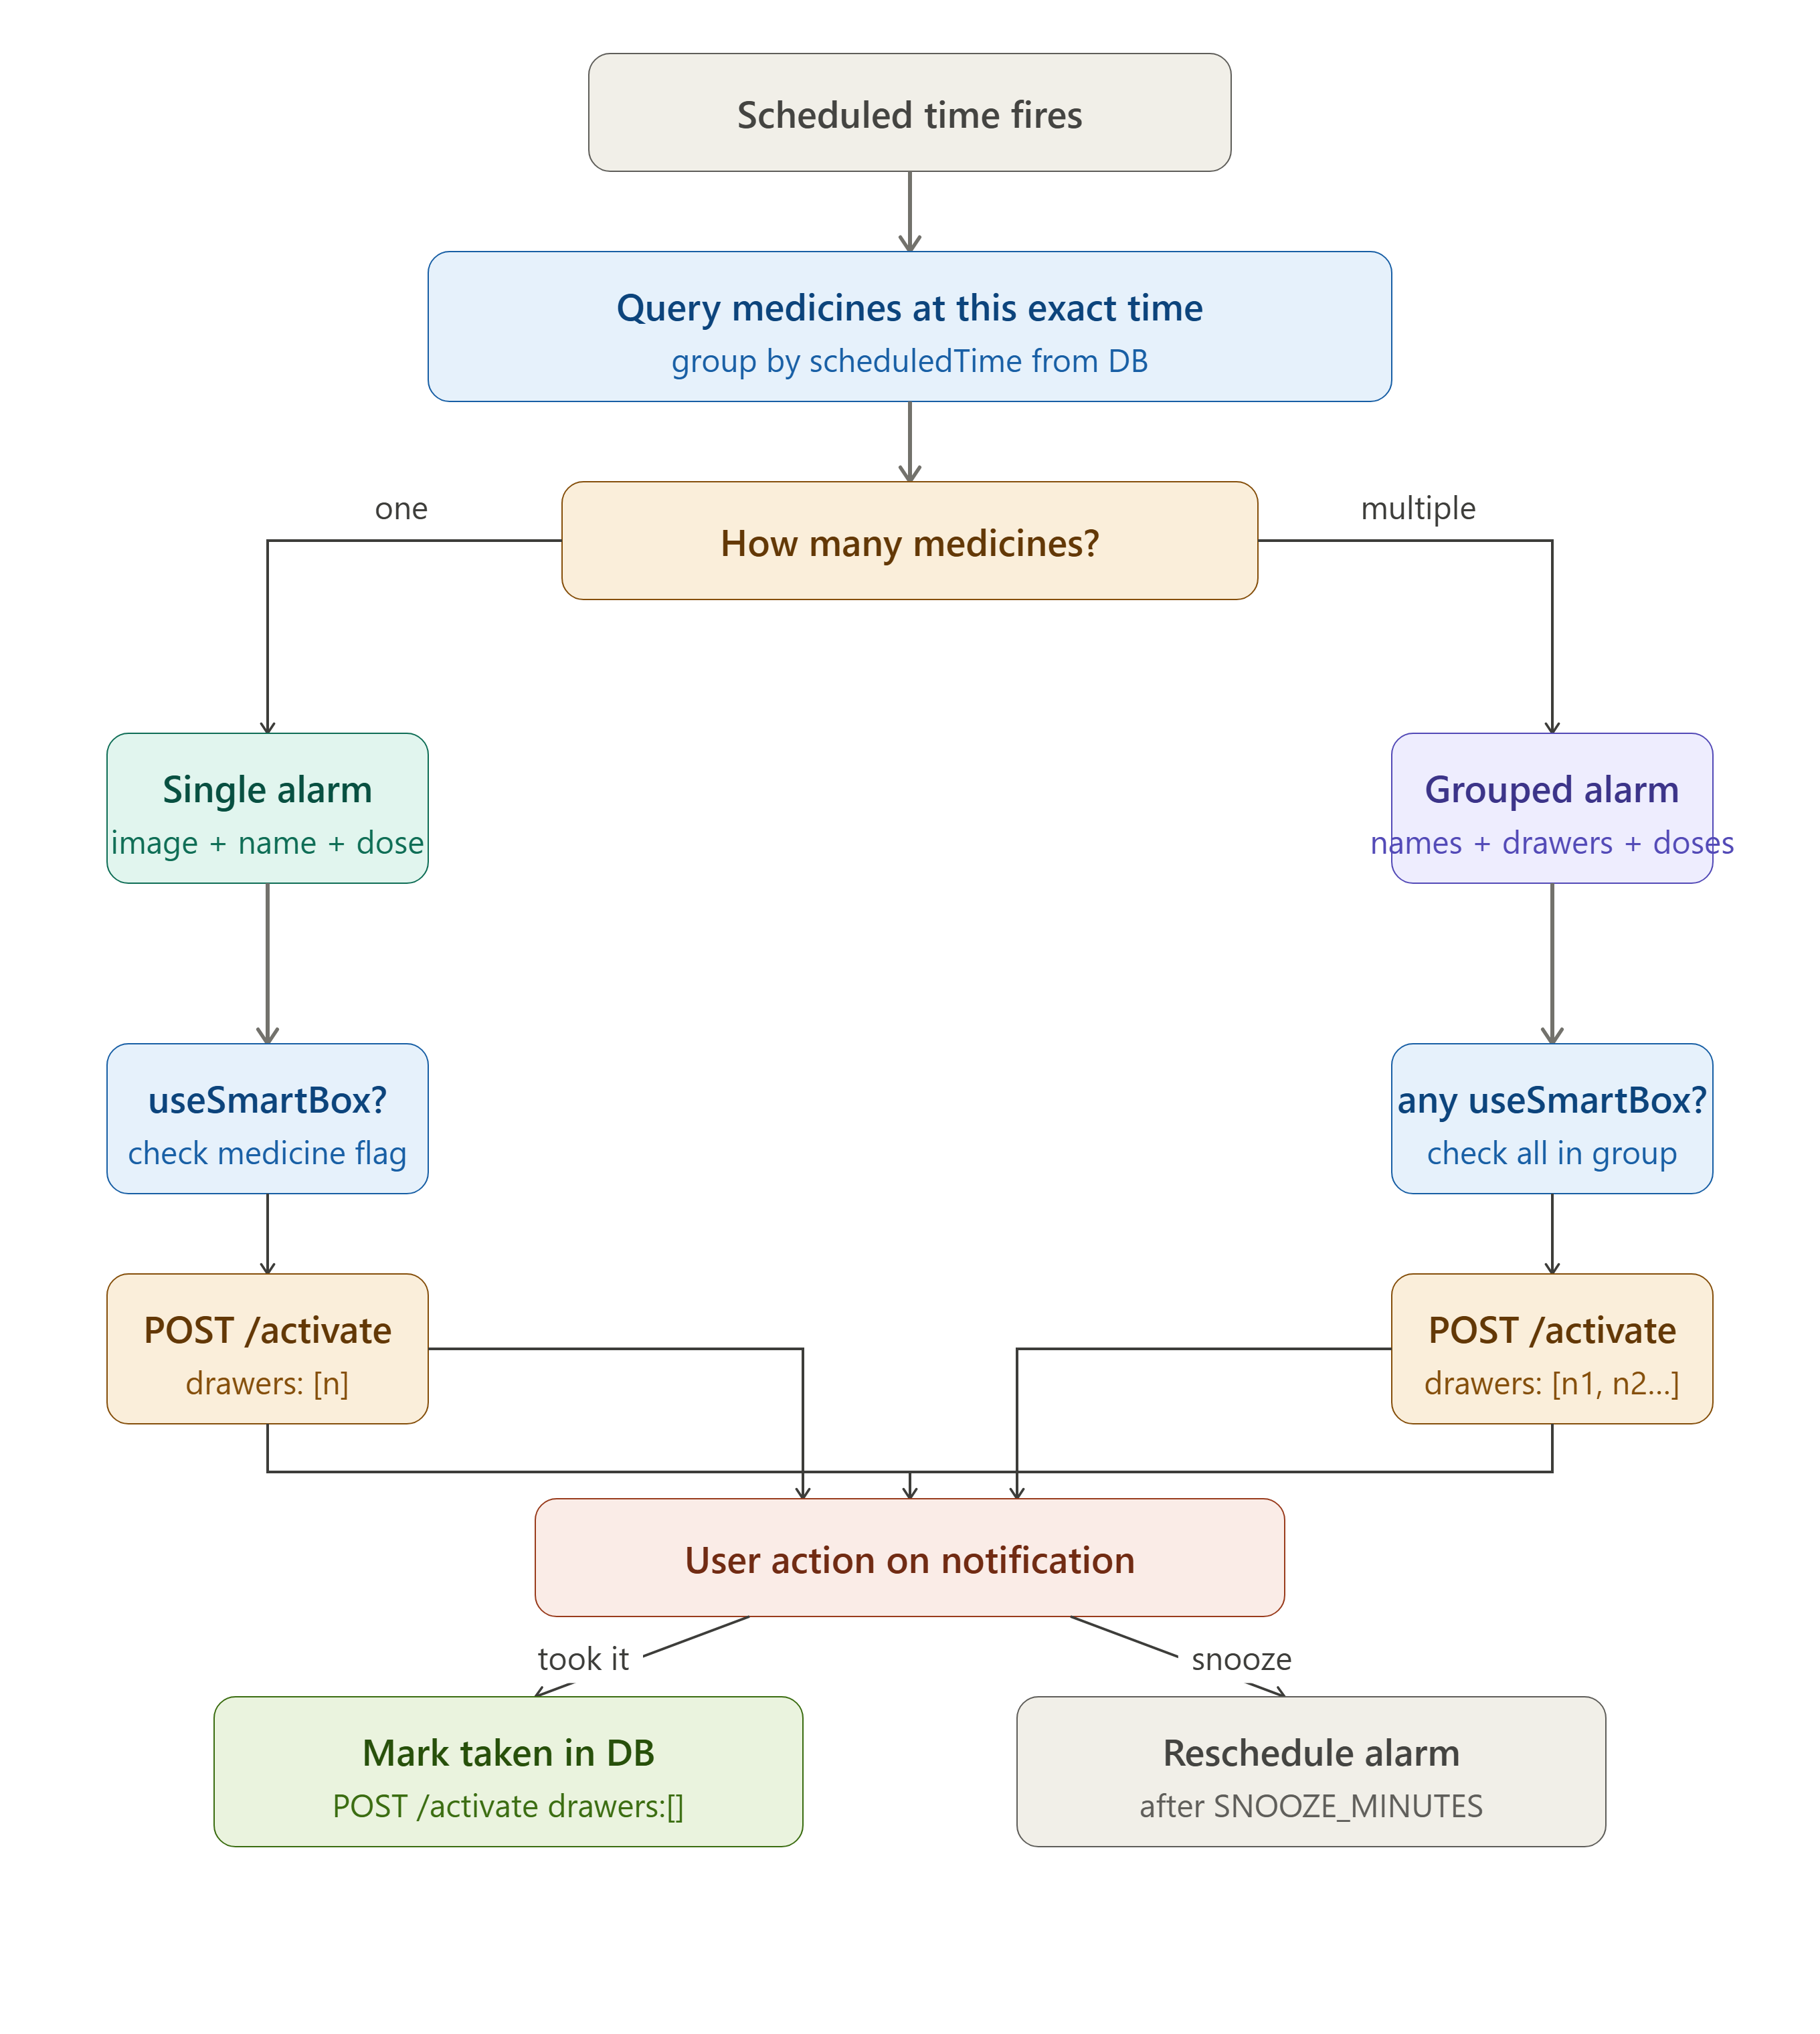
\includegraphics[width=0.72\linewidth]{alarm_trigger_flow.png}
\caption{Medication alarm decision tree, including grouping of multiple
medications due at the same time into one drawer-activation call.}
\label{fig:alarmtree}\end{figure}

\section{Symptom-Triage Flow}

The symptom checker exists in two parallel implementations, both reachable from
the running app (Figure~\ref{fig:symflow}). The legacy v1 flow is a free-text /
flat-symptom classifier with no urgency logic; the structured v2 flow is a
five-step wizard whose result is jointly determined by the LightGBM classifier
(for the disease prediction) and the rule engine (for red flags and urgency),
with the rule engine able to escalate but never suppress urgency.

\begin{figure}[H]
\centering
\resizebox{\linewidth}{!}{%
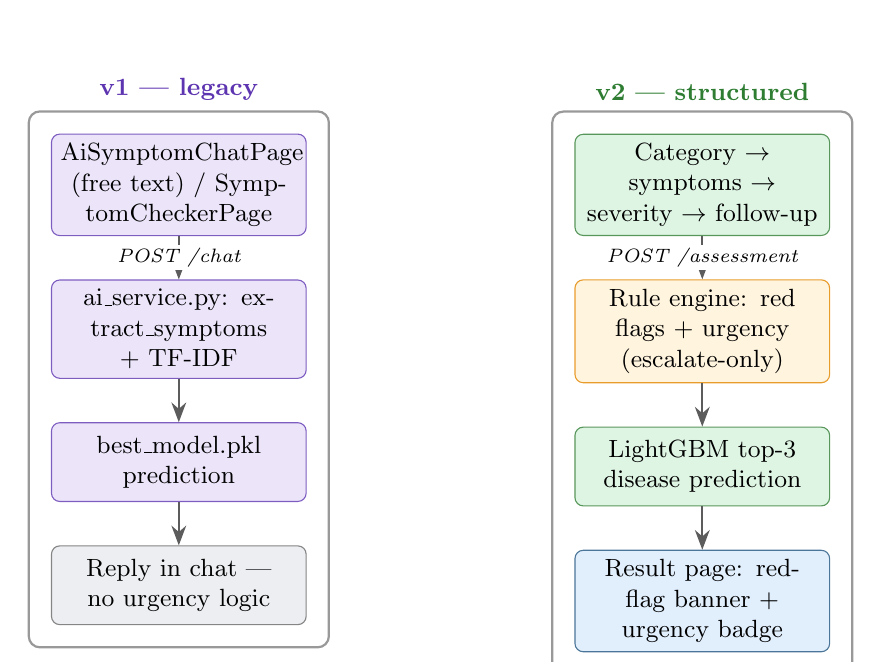
\begin{tikzpicture}[font=\scriptsize, node distance=0.55cm and 0.8cm]
% v1
\node[pbox, text width=3.0cm] (a1) {AiSymptomChatPage (free text) / SymptomCheckerPage};
\node[pbox, below=of a1, text width=3.0cm] (a2) {ai\_service.py: extract\_symptoms + TF-IDF};
\node[pbox, below=of a2, text width=3.0cm] (a3) {best\_model.pkl prediction};
\node[graybox, below=of a3, text width=3.0cm] (a4) {Reply in chat --- no urgency logic};
\draw[flow] (a1) -- node[lbl]{POST /chat} (a2);
\draw[flow] (a2) -- (a3);
\draw[flow] (a3) -- (a4);
\begin{scope}[on background layer]
\node[layer, fit=(a1)(a4), label={[font=\small\bfseries\color{softpurple}]above:v1 --- legacy}] {};
\end{scope}

% v2
\node[gbox, right=3.4cm of a1, text width=3.0cm] (c1) {Category $\rightarrow$ symptoms $\rightarrow$ severity $\rightarrow$ follow-up};
\node[abox, below=of c1, text width=3.0cm] (c2) {Rule engine: red flags + urgency (escalate-only)};
\node[gbox, below=of c2, text width=3.0cm] (c3) {LightGBM top-3 disease prediction};
\node[box, below=of c3, text width=3.0cm] (c4) {Result page: red-flag banner + urgency badge};
\draw[flow] (c1) -- node[lbl]{POST /assessment} (c2);
\draw[flow] (c2) -- (c3);
\draw[flow] (c3) -- (c4);
\begin{scope}[on background layer]
\node[layer, fit=(c1)(c4), label={[font=\small\bfseries\color{softgreen}]above:v2 --- structured}] {};
\end{scope}
\end{tikzpicture}
}%
\caption{The two coexisting symptom-checker flows. v1 has no safety layer; v2
runs the ML prediction and the rule engine independently and reflects the more
severe of the two.}
\label{fig:symflow}
\end{figure}

\subsection{The Safety Rule Engine}
\label{sec:ruleengine}

Two pure-function rule modules sit between the raw assessment input and the
final result, and --- per an explicit design rule in the code --- \textbf{the
rule engine can only escalate urgency, never suppress it}:

\begin{itemize}[leftmargin=1.4em]
  \item \texttt{red\_flag\_rules} --- most red-flag symptoms trigger at severity
  $\ge 2$; syncope and loss-of-consciousness variants trigger at any severity
  $\ge 1$, reflecting their inherent urgency.
  \item \texttt{urgency\_rules} --- combines red flags with a vitals-derived
  floor into one of four levels: \emph{critical} (any red flag at severity
  $\ge 3$, or critical vitals), \emph{high} (any red flag, or high vitals),
  \emph{moderate} ($\ge 2$ moderate-severity symptoms, or known hypertension
  with elevated vitals), or \emph{low}.
  \item \texttt{bp\_rules} --- the single shared source of BP/SpO2/HR thresholds,
  written to be the one place these numbers live rather than duplicated between
  the symptom checker and the BP feature's own alerting.
\end{itemize}

When an assessment is launched from a concerning BP reading specifically, and
the result comes back moderate or high (not yet critical), the response
additionally recommends resting five minutes and re-measuring rather than
escalating immediately --- the concrete implementation of the ``re-measure on a
borderline high reading, notify immediately on a confirmed critical one''
policy.

\section{Application Screenshots}
\label{sec:screenshots}

The screens below are grouped as complete user flows, captured with the app set
to \textbf{Arabic}, so the sequence itself is direct proof that the interface
runs fully and naturally right-to-left --- not just isolated screens.

\subsection*{Flow 1 --- Guided blood-pressure measurement}

\begin{figure}[H]\centering
\flowshot{0.235}{screen_bp_1_setup.png}{(a) Sensor setup / placement}\hfill
\flowshot{0.235}{screen_bp_2_measuring.png}{(b) Live measuring (finger/leads)}\hfill
\flowshot{0.235}{screen_bp_3_result.png}{(c) Result / cuff confirmation}\hfill
\flowshot{0.235}{screen_bp_4_history.png}{(d) History \& trend}
\caption{Guided blood-pressure measurement, from sensor setup to saved history
(Arabic UI).}
\label{fig:flow-bp}
\end{figure}

\subsection*{Flow 2 --- Medication, from setup to alarm}

\begin{figure}[H]\centering
\flowshot{0.235}{screen_med_1_list.png}{(a) Medications list}\hfill
\flowshot{0.235}{screen_med_2_form.png}{(b) Add-medicine form}\hfill
\flowshot{0.235}{screen_med_3_box.png}{(c) Smart-box drawer setup}\hfill
\flowshot{0.235}{screen_med_4_alarm.png}{(d) Medication alarm}
\caption{Medication flow: list, add-medicine form, smart-box setup, and the
resulting alarm (Arabic UI).}
\label{fig:flow-med}
\end{figure}

\subsection*{Flow 3 --- Symptom triage}

\begin{figure}[H]\centering
\flowshot{0.185}{screen_sym_1_category.png}{(a) Category}\hfill
\flowshot{0.185}{screen_sym_2_symptoms.png}{(b) Symptoms}\hfill
\flowshot{0.185}{screen_sym_3_severity.png}{(c) Severity}\hfill
\flowshot{0.185}{screen_sym_4_followup.png}{(d) Follow-up}\hfill
\flowshot{0.185}{screen_sym_5_result.png}{(e) Result + urgency}
\caption{Symptom-triage wizard: category, symptoms, severity, follow-up, and
the urgency-graded result (Arabic UI).}
\label{fig:flow-sym}
\end{figure}

\subsection*{Flow 4 --- Communication}

Reaching a linked patient or caregiver directly from the app, including the
dedicated emergency-call entry point (Figure~\ref{fig:flow-call}).

\begin{figure}[H]\centering
\flowshot{0.235}{screen_call_1_outgoing.png}{(a) Outgoing call}\hfill
\flowshot{0.235}{screen_call_2_incoming.png}{(b) Incoming call}\hfill
\flowshot{0.235}{screen_call_3_active.png}{(c) In-call screen}\hfill
\flowshot{0.235}{screen_call_4_emergency.png}{(d) Emergency call}
\caption{WebRTC audio/video calling: outgoing, incoming, active call, and the
emergency-call screen (Arabic UI).}
\label{fig:flow-call}
\end{figure}

\subsection*{Core screens}

\begin{figure}[H]\centering
\flowshot{0.235}{screen_home_patient.png}{(a) Patient home}\hfill
\flowshot{0.235}{screen_home_caregiver.png}{(b) Caregiver / patient detail}\hfill
\flowshot{0.235}{screen_notifications.png}{(c) Notifications inbox}\hfill
\flowshot{0.235}{screen_linking_qr.png}{(d) Caregiver linking (QR)}
\caption{Patient home, caregiver patient detail, notifications inbox, and
QR-based caregiver linking (Arabic UI).}
\label{fig:flow-core}
\end{figure}


%==============================================================================
\chapter{Impact}
%==============================================================================

\section{Target Audience}

The primary users are patients managing chronic cardiovascular conditions at
home and the family members or informal carers who monitor them remotely.
The system deliberately does \emph{not} model a clinical-staff or clinic-admin
role: \texttt{UserRole} is a two-value enum (\texttt{patient},
\texttt{caregiver}), and no schema, endpoint, or screen anywhere in the
codebase suggests a broader role model was ever built or even partially
scaffolded. Its scope is patient-and-family, not patient-and-provider, and that
scoping decision shapes every screen in the app: there is no clinician
dashboard to design around, no multi-tenant clinic account to secure, and no
provider-facing reporting format to satisfy --- the entire interface can be
optimized for exactly two perspectives on the same underlying data. Three
concrete groups of people benefit directly from that focus, and the specific
design choices throughout the app map onto their real daily difficulties
rather than a generic ``health app'' feature list:

\begin{itemize}[leftmargin=1.4em]
  \item \textbf{Elderly patients managing hypertension.} Older adults are both
  the demographic most likely to live with hypertension and the demographic
  least well served by an app designed primarily for younger, tech-fluent
  users. Health Mate answers this directly: a large, simple UI; a
  step-by-step guided measurement that removes any guesswork about how to
  attach and use the sensor correctly; scheduled reminders so the patient
  never has to hold a measurement schedule in their own head; and full Arabic
  support with right-to-left layout, so language is never the reason a patient
  cannot use the app. A normal cuff measurement actually asks an older patient
  to get three separate things right --- correct cuff placement, sitting still
  for an accurate reading, and then remembering to write the number down
  somewhere --- and any one of the three going wrong can mean the reading is
  skipped entirely. The guided flow collapses all three into a single prompted
  routine, so there is no step left for the patient to get wrong on their own.
  \item \textbf{Any hypertension patient who needs to track their condition.}
  For the broader population managing high blood pressure, day to day, the
  value is continuity rather than any single reading. Instead of isolated
  clinic snapshots taken weeks or months apart, the patient accumulates a real,
  continuous history that they and their caregiver can both see, and --- most
  importantly for actual safety --- a critical reading is escalated to a
  linked caregiver automatically and immediately, rather than depending on the
  patient themselves noticing the danger, judging its severity correctly, and
  then finding the presence of mind to raise the alarm while acutely unwell.
  The per-patient calibration layer means the numbers this patient sees become
  progressively more trustworthy specifically for their own physiology over
  time, rather than only being accurate on average across the population the
  underlying model was trained on.
  \item \textbf{Patients with dementia or Alzheimer's who need medication
  support.} Memory-impairment patients face a distinct problem that the
  blood-pressure features do not address at all: not \emph{measuring}
  anything, but \emph{remembering which medication to take, and when}. The
  smart medicine box speaks directly to this gap. Rather than relying on the
  patient to hold a schedule in memory, it lights the LED for exactly the
  drawer that is due right now (and sounds a buzzer), turning an abstract fact
  --- ``it is 8\,pm, time for the evening dose'' --- into an unambiguous
  physical pointer at one specific compartment, reinforced at the same moment
  by a phone notification. For a patient who cannot reliably retain a
  schedule, a device that points directly at the answer is materially more
  usable than one that only reminds them a decision is due and leaves them to
  work out which pill that means on their own. A linked caregiver sees the
  resulting adherence log, so a missed dose is visible to someone who is in a
  position to follow up, rather than silently going unnoticed.
\end{itemize}

\section{Problems Solved}

The table below restates the same value proposition as a direct map from a
concrete, real-world problem to the specific mechanism in the running system
that addresses it --- deliberately including a few smaller but genuinely useful
mechanisms (offline caching, the emergency-call screen) that are easy to
overlook next to the two headline AI features, but that materially affect
whether the app is actually usable in the situations patients and caregivers
run into day to day.

\begin{table}[H]
\centering
\caption{Real-world problems and the Health Mate mechanism that solves each.}
\label{tab:problems}
\small
\begin{tabularx}{\linewidth}{@{}>{\raggedright\arraybackslash}p{4.7cm}Y@{}}
\toprule
\textbf{Problem} & \textbf{How Health Mate addresses it} \\
\midrule
Patients skip or forget blood-pressure measurement &
Up to three scheduled daily reminders, paired with a guided, low-friction
sensor flow that requires no manual cuff technique at all \\
A dangerous reading goes unnoticed until it becomes an emergency &
Automatic risk-tier classification with a rate-limited emergency push
notification sent to every linked caregiver the moment a high or critical
reading is recorded \\
Caregivers have no visibility into a patient's condition without asking &
A live, linked view of the patient's vitals, calibration status, and
medication adherence, requiring no ongoing action from the patient after the
initial link is made \\
A cuff reading is intimidating or physically hard for an elderly patient to
self-administer correctly &
An 8-second cuffless sensor capture, walked through step by step, with live
finger/lead feedback so a bad measurement attempt is caught and corrected
before a reading is even taken \\
A model trained on a general population is inaccurate for one specific
individual &
A per-patient calibration layer that adapts to occasional reference cuff
readings and automatically detects when its own fit has drifted out of date \\
Dementia/Alzheimer's patients forget which medication to take, and when &
The smart medicine box lights a per-drawer LED (with a buzzer) pointing at the
exact compartment due right now, reinforced by a phone alarm \\
There is no record of whether a medication dose was actually taken &
An adherence log with optional photo proof, visible to the linked caregiver \\
Reaching help quickly during a frightening reading or symptom episode &
In-app WebRTC audio/video calling, including a dedicated emergency-call screen
between patient and caregiver \\
Symptoms that may be urgent are self-judged by an unwell, possibly panicking
patient &
A structured symptom-triage wizard backed by a rule engine that can escalate
urgency independently of the ML prediction and can never suppress a red flag,
regardless of what the model predicts \\
Arabic-speaking users are treated as a secondary market by most health apps &
Full English/Arabic parity at the translation-key level, right-to-left
layout, and translated reminders and alerts, not just translated static text \\
Losing access to recent data the moment connectivity drops &
Offline-first caching of the last known reading and history, with local
reminders that continue to fire even with no network connection at all \\
\bottomrule
\end{tabularx}
\end{table}

\section{Innovative Aspects of the Design}

\begin{itemize}[leftmargin=1.4em]
  \item A genuinely \textbf{fault-tolerant, resumable model-training pipeline},
  built out of practical necessity for training on a quota-limited shared GPU
  platform, in which every stage checkpoints and one model's failure never takes
  down the run.
  \item A \textbf{calibration subsystem} that adapts a population-trained model
  to an individual patient without retraining it, upgrading its own fit quality
  automatically as more reference data accumulates.
  \item A \textbf{safety rule engine} architecturally guaranteed to only
  escalate, never suppress, urgency relative to the ML model's own output.
  \item A \textbf{single shared feature-engineering implementation} used by both
  training and production inference on both AI subsystems, eliminating
  train/inference drift by construction.
  \item A \textbf{clean separation of clinical logic from hardware}: the devices
  are pure collectors/actuators, and every safety-relevant decision runs in one
  auditable backend.
\end{itemize}

\section{Reliability}

Reliability was treated as a first-class concern in the parts of the system that
matter most. The BP model service and the smart-box hardware client both fail
soft rather than raising on a missing model or unreachable device. The rule
engine, calibration service, and drift detector each carry dedicated unit tests
--- the backend's test investment is concentrated on exactly the newest,
safety-critical code (a rule-engine test suite, BP endpoint and drift tests,
assessment and LLM-fallback tests, a Redis chat-session test, and an automated
Arabic-encoding audit), rather than spread evenly.

Where reliability gaps remain, this documentation states them directly rather
than implying a finished, hardened system:

\begin{itemize}[leftmargin=1.4em]
  \item \textbf{Session/token revocation is not implemented} --- logout and
  refresh do not invalidate anything server-side; this is a standard stateless
  JWT tradeoff, stated in the code's own docstring.
  \item \textbf{The caregiver-linking QR flow is unencrypted} --- the QR code
  carries a plain user UUID with no signing or expiry.
  \item \textbf{The generic sensor endpoints always return simulated data},
  regardless of IoT mode, which could be mistaken for a live feed if read from
  the API surface alone.
\end{itemize}

\section{Added Value}

For a patient, the system converts BP monitoring from an easy-to-skip manual
task into a scheduled, guided routine with a direct line to a caregiver in an
emergency. For a caregiver, it converts remote monitoring from ``wait to be
told'' into a live, linked view with automatic alerting. The bilingual,
RTL-aware design makes both experiences equally first-class in Arabic and
English, which materially broadens the population the system can actually serve.

%==============================================================================
\chapter{Conclusions}\label{sec:conclusion}
%==============================================================================

Health Mate is a working, end-to-end remote-monitoring system spanning custom
sensor hardware, two trained AI models, a FastAPI backend that centralizes every
safety decision, and a bilingual Flutter app serving both patients and
caregivers from shared infrastructure. The blood-pressure model clears the
clinical standard for diastolic pressure but not yet for systolic; the
symptom-checker model reaches strong top-3 accuracy overall but is weakest
precisely on the cardiac subtypes most relevant to the project's focus. Both
results are reported as measured, not adjusted for presentation.

The project's biggest lesson, encountered independently in both AI subsystems,
was that a more sophisticated architecture does not automatically outperform a
simpler one on a given dataset, and that discovering this requires actually
running the simpler baseline rather than assuming the more complex model is
better by construction. A second, quieter lesson concerns engineering
discipline: sharing one preprocessing and feature-engineering implementation
between training and inference, failing soft on every best-effort integration,
and keeping the safety layer as pure, testable functions independent of the ML
model together produced a system whose behavior can be reasoned about and
trusted at its most safety-critical points.

Above all, the project was documented honestly. Every headline number is the one
the code actually produces, every architectural gap is named, and every
inconclusive result is left inconclusive rather than rounded up. This is the
posture a real medical product demands, and adopting it at the graduation-project
stage is itself part of the contribution.

%==============================================================================
\chapter{Future Directions}
%==============================================================================

\begin{itemize}[leftmargin=1.4em]
  \item \textbf{Validate the BP model against real hardware.} Collect
  MAX30102/AD8232 recordings alongside reference cuff readings and measure the
  model's actual MAE on that data --- the single largest open validation
  question, and one that lies in the absence of a measurement rather than in the
  code.
  \item \textbf{Re-run the calibration effectiveness study} using genuinely
  time-separated reference readings that mirror how the deployed service
  accumulates samples, rather than adjacent overlapping windows from one
  recording.
  \item \textbf{Investigate the complexity paradox.} Determine why additional
  architectural sophistication underperformed a simpler baseline in both
  subsystems --- candidates include insufficient data diversity for attention to
  earn its parameters, and an inductive-bias mismatch for fixed-length windows.
  \item \textbf{Strengthen cardiac-subtype discrimination.} Collect real
  (non-synthetic) patient assessment data and apply the same targeted
  differentiation to overlapping cardiac classes that was applied to the
  respiratory and neurological triads.
  \item \textbf{Close the backend security gaps} --- server-side session/token
  revocation and cryptographic protection (signing + expiry) for the
  caregiver-linking flow --- before any production deployment.
  \item \textbf{Harden device provisioning} --- replace the hardcoded firmware
  device token with a per-device provisioned secret.
  \item \textbf{Decide the long-term status of the legacy v1 symptom checker}
  now that a safer, structured v2 flow exists alongside it, and consider the
  taxonomy's own anticipated ``Phase 6'' move to a Postgres-backed repository.
\end{itemize}

\section{Hardware Sensor Upgrade Path}

The current prototype uses two low-cost breakout modules --- a MAX30102 PPG
sensor and an AD8232 single-lead ECG front-end --- chosen for availability and
price during development. Both are functional but are consumer/fitness-grade
parts, and a clear, researched upgrade path exists toward medical-grade signal
acquisition, which is the most direct lever on the SBP accuracy gap identified
in Chapter~\ref{sec:results}:

\begin{itemize}[leftmargin=1.4em]
  \item \textbf{Combine PPG and ECG into one medical-grade module.} The
  \textbf{MAX86150}~\cite{max86150} integrates a PPG sensor \emph{and} a
  single-lead ECG channel in one part with a shared, synchronized analog front
  end. This directly replaces \emph{both} current sensors, removes the
  cross-module timing uncertainty that affects the pulse-transit-time feature,
  and has been reported in cuffless-BP evaluations at a mean error on the order
  of $\pm$5.3\,mmHg systolic and $\pm$2.8\,mmHg diastolic --- squarely in the
  range that would move the systolic result toward the AAMI bar.
  \item \textbf{Upgrade the ECG front end.} If PPG and ECG are kept separate,
  the \textbf{MAX30003}~\cite{max30003} is a medical-grade biopotential AFE with
  built-in EMI filtering, DC lead-off detection, internal lead biasing, and
  ultra-low power draw --- a substantial signal-quality improvement over the
  AD8232's motion-artifact-tolerant but fitness-oriented design.
  \item \textbf{Adopt a validated reference design.} Vendor cuffless-BP
  reference designs such as the \textbf{MAXREFDES220}~\cite{maxrefdes} are
  documented to meet Class-II regulatory accuracy limits under the
  \textbf{ISO 81060-2}~\cite{aami} clinical-validation standard, and could serve
  as a hardware baseline to validate the trained model against, closing the
  real-hardware validation gap named above.
\end{itemize}

Pairing any of these upgrades with the real-hardware data-collection step above
would let the model be retrained and re-validated on higher-fidelity signals
from the actual target population, which is the single change most likely to
turn the systolic result from an indicative trend into a diagnostic-grade
reading.

%==============================================================================
\begin{thebibliography}{99}
\addcontentsline{toc}{chapter}{References}
%==============================================================================
\bibitem{mimic3} A. E. W. Johnson, T. J. Pollard, L. Shen, et al.,
``MIMIC-III, a freely accessible critical care database,''
\textit{Scientific Data}, vol. 3, art. 160035, 2016.
doi:10.1038/sdata.2016.35.

\bibitem{kachuee2015} M. Kachuee, M. M. Kiani, H. Mohammadzade, and M. Shabany,
``Cuff-less high-accuracy calibration-free blood pressure estimation using pulse
transit time,'' in \textit{Proc. IEEE Int. Symp. Circuits and Systems (ISCAS)},
2015, pp. 1006--1009.

\bibitem{ppgbp2021} F. Schrumpf, P. Frenzel, C. Aust, G. Osterhoff, and M. Fuchs,
``Assessment of deep learning based blood pressure prediction from PPG and rPPG
signals,'' in \textit{Proc. IEEE/CVF CVPR Workshops}, 2021.
arXiv:2104.09313.

\bibitem{ppgdl2021} S. Baker, W. Xiang, and I. Atkinson,
``A deep learning approach to predict blood pressure from PPG signals,''
\textit{Computers in Biology and Medicine}, 2021. arXiv:2108.00099.

\bibitem{lightgbm} G. Ke, Q. Meng, T. Finley, et al.,
``LightGBM: A highly efficient gradient boosting decision tree,'' in
\textit{Advances in Neural Information Processing Systems (NeurIPS)}, vol. 30,
2017.

\bibitem{attention} A. Vaswani, N. Shazeer, N. Parmar, et al.,
``Attention is all you need,'' in \textit{Advances in Neural Information
Processing Systems (NeurIPS)}, vol. 30, 2017.

\bibitem{blandaltman} J. M. Bland and D. G. Altman,
``Statistical methods for assessing agreement between two methods of clinical
measurement,'' \textit{The Lancet}, vol. 327, no. 8476, pp. 307--310, 1986.

\bibitem{bhs} E. O'Brien, J. Petrie, W. Littler, et al.,
``The British Hypertension Society protocol for the evaluation of automated and
semi-automated blood pressure measuring devices,''
\textit{Journal of Hypertension}, vol. 11 (suppl. 2), pp. S43--S62, 1993.

\bibitem{aami} Association for the Advancement of Medical Instrumentation,
\textit{ANSI/AAMI/ISO 81060-2: Non-invasive Sphygmomanometers --- Clinical
Investigation of Automated Measurement Type}.

\bibitem{tcn} S. Bai, J. Z. Kolter, and V. Koltun,
``An empirical evaluation of generic convolutional and recurrent networks for
sequence modeling,'' arXiv:1803.01271, 2018.

\bibitem{lstm} S. Hochreiter and J. Schmidhuber,
``Long short-term memory,'' \textit{Neural Computation}, vol. 9, no. 8,
pp. 1735--1780, 1997.

\bibitem{layernorm} J. L. Ba, J. R. Kiros, and G. E. Hinton,
``Layer normalization,'' arXiv:1607.06450, 2016.

\bibitem{max86150} Maxim Integrated (Analog Devices),
\textit{MAX86150 Integrated Photoplethysmogram and Electrocardiogram Bio-Sensor
Module for Mobile Health}, Datasheet.

\bibitem{max30003} Maxim Integrated (Analog Devices),
\textit{MAX30003 Ultra-Low Power, Single-Channel Integrated Biopotential (ECG,
R-to-R Detection) Analog Front End}, Datasheet.

\bibitem{maxrefdes} Maxim Integrated (Analog Devices),
\textit{MAXREFDES220\# --- Cuffless Blood-Pressure Measurement Reference
Design}, meeting Class-II regulatory accuracy limits (ISO 81060-2).
\end{thebibliography}


%==============================================================================
\appendix
\chapter{API Endpoint Reference}
%==============================================================================

All endpoints are under the base path \texttt{/api/v1}. Two authentication
schemes coexist: \textbf{Bearer JWT} for all human-user endpoints, and
\textbf{device headers} (\texttt{X-Device-ID} + \texttt{X-Device-Token}) for the
two BP hardware endpoints only.

\begin{longtable}{@{}>{\raggedright\arraybackslash}p{4.6cm}>{\raggedright\arraybackslash}p{1.6cm}>{\raggedright\arraybackslash}p{8.2cm}@{}}
\caption{REST API surface, grouped by router.}\label{tab:api}\\
\toprule
\textbf{Endpoint} & \textbf{Method} & \textbf{Purpose} \\
\midrule
\endfirsthead
\multicolumn{3}{c}{\small\itshape Table~\ref{tab:api} continued}\\
\toprule
\textbf{Endpoint} & \textbf{Method} & \textbf{Purpose} \\
\midrule
\endhead
\bottomrule
\endfoot
\multicolumn{3}{@{}l}{\textit{\textbf{Authentication (/auth)}}}\\
/auth/register & POST & Create a patient or caregiver account \\
/auth/login & POST & Email/password login, returns access + refresh tokens \\
/auth/refresh & POST & Exchange a refresh token for a new pair \\
/auth/social & POST & Firebase-based login/signup \\
/auth/verify-email & POST & Mark email verified \\
/auth/logout & POST & Returns success; no server-side invalidation (known gap) \\
\multicolumn{3}{@{}l}{\textit{\textbf{Users (/users)}}}\\
/users/me & GET/PUT/DELETE & Current user profile management \\
/users/me/fcm-token & PUT & Register/update push token \\
/users/me/password & PUT & Change password \\
/users/linked & GET & Linked caregivers or patients \\
/users/link/\{id\} & POST & Link with another user by ID \\
/users/linked/\{id\} & DELETE & Deactivate a link \\
\multicolumn{3}{@{}l}{\textit{\textbf{Vitals / Blood pressure (/vitals)}}}\\
/vitals/bp & POST & Manual BP entry \\
/vitals/bp/submit & POST & Device submits 800-sample window; model + calibration \\
/vitals/bp/complete & POST & Patient supplies cuff reading, records calibration sample \\
/vitals/bp/heartbeat & POST & Device reports finger/lead status \\
/vitals/bp/history & GET & Paginated reading history \\
/vitals/bp/stats & GET & Aggregate statistics for charts \\
/vitals/patient/\{id\}/* & GET & Same views for a linked patient (caregiver) \\
\multicolumn{3}{@{}l}{\textit{\textbf{Medications, reminders, notifications}}}\\
/medications & CRUD & Catalog, schedule, smart-box assignment, adherence \\
/bp\_reminders/schedule-daily & POST & Derive up to 3 daily BP reminder times \\
/notifications & GET/PUT/DELETE & Inbox, unread-count, mark-read, delete \\
/contacts & CRUD & Medical contacts \\
\multicolumn{3}{@{}l}{\textit{\textbf{Calls (/calls)}}}\\
/calls & POST & Start a call \\
/calls/\{id\}/offer,accept,reject,busy,end & POST & WebRTC session lifecycle \\
\multicolumn{3}{@{}l}{\textit{\textbf{IoT / Hardware}}}\\
/iot/sensors/status, /data & GET & Simulated sensor telemetry (mock, always) \\
/iot/medicine-box/* & GET/POST & Real ESP32 medicine-box state and control \\
/hardware/status & GET & ESP32 reachability ping \\
\multicolumn{3}{@{}l}{\textit{\textbf{AI / Symptom checker (/ai)}}}\\
/ai/symptom-checker, /chat & POST & v1 legacy classifier + free-text chat \\
/ai/categories, /taxonomy/symptoms & GET & v2 taxonomy \\
/ai/assessment & POST & v2 structured assessment \\
/ai/bp-triage & POST & v2 assessment + borderline-high re-measure override \\
/ai/chat/from-assessment & POST & Seed a chat session with assessment context \\
/ai/assessment/notify-caregiver & POST & Explicit caregiver notification trigger \\
/ai/assessment/rollout-metrics & GET & Live counters: count, red-flag rate, latency \\
\multicolumn{3}{@{}l}{\textit{\textbf{Upload / Realtime}}}\\
/upload/* & POST/DELETE & Cloudinary-backed image upload \\
/ws, /socket.io & WS & JWT-authenticated WebRTC signaling events \\
\end{longtable}

% --------------------------------------------------------------------------
% Screenshot file map (author reference only -- intentionally not typeset,
% so no placeholder/guide chapter appears in the compiled PDF for reviewers).
% Set the app to Arabic, capture each screen below, and drop the file into
% assets/branding/ -- every \flowshot / \screenshot slot in this document
% picks it up automatically, no further edits needed.
%
% Flow 1 - Guided BP measurement (fig:flow-bp)
%   screen_bp_1_setup.png       BPMeasurementGuidePage - sensor placement step
%   screen_bp_2_measuring.png   BPMeasurementGuidePage - live measuring state
%   screen_bp_3_result.png      BPMeasurementGuidePage - result / cuff entry
%   screen_bp_4_history.png     BPHistoryPage           - history / trend
% Flow 2 - Medication to alarm (fig:flow-med)
%   screen_med_1_list.png       MedicationsPage         - medication list
%   screen_med_2_form.png       MedicineFormPage        - add-medicine form
%   screen_med_3_box.png        MedicationBoxPage       - smart-box setup
%   screen_med_4_alarm.png      MedicationAlarmPage     - full-screen alarm
% Flow 3 - Symptom triage (fig:flow-sym)
%   screen_sym_1_category.png   CategorySelectionPage
%   screen_sym_2_symptoms.png   SymptomSelectionPage
%   screen_sym_3_severity.png   SymptomSeverityPage
%   screen_sym_4_followup.png   FollowupQuestionsPage
%   screen_sym_5_result.png     AssessmentResultPage    - urgency + red flags
% Flow 4 - Communication / calling (fig:flow-call)
%   screen_call_1_outgoing.png  CallPage (outgoing)
%   screen_call_2_incoming.png  IncomingCallPage
%   screen_call_3_active.png    CallPage (in-call)
%   screen_call_4_emergency.png EmergencyCallActionPage
% Core screens (fig:flow-core)
%   screen_home_patient.png     PatientHomePage
%   screen_home_caregiver.png   CaregiverPatientDetailPage
%   screen_notifications.png    NotificationsPage
%   screen_linking_qr.png       QrCodePage / QrScannerPage
% --------------------------------------------------------------------------

\chapter{Deployment and Networking}

The system runs via a single \texttt{docker-compose.yml} (PostgreSQL, Redis, and
the FastAPI API container) on one host --- a development/demo topology with no
staging/production split, no reverse proxy/TLS, and no orchestration. The
\texttt{Symptom-Checker/} and \texttt{Predict-ABP/} directories are bind-mounted
into the API container rather than copied at build time, so model artifacts can
be swapped without rebuilding the image.

Networking between the phone, backend, and both ESP devices depends on all being
on the same WiFi network, with IP addresses hardcoded in four separate files
that must be updated by hand when the network changes: the frontend API base URL
and ESP32 constant, the backend's ESP32 IP setting, and the BP firmware's server
URL. This is a real, hand-maintained coupling and a documented operational step,
not an oversight.

\chapter{Documentation Method and Honesty Statement}

Every factual claim in this document was produced by reading primary sources
directly, in priority order: (1)~source code --- Python backend modules, Dart
widgets and providers, Arduino/ESP firmware, SQLAlchemy models, Pydantic
schemas, and Alembic migrations; (2)~generated artifacts --- model metadata
JSON, evaluation reports, result CSVs, and the training notebook's own cell
outputs, treated as primary evidence because they are produced by running code,
not by describing intent; and (3)~direct cross-verification, where a claim that
could be checked on two sides (for example, whether the linking QR code encodes
an encrypted payload) was read on both the backend and the Flutter side rather
than trusting one comment.

Several claims from earlier project materials were corrected during this review:
the blood-pressure model is a 1D-CNN, not an LSTM; the production symptom-checker
model is LightGBM over structured features, with an older TF-IDF pipeline still
running in parallel rather than in its place; the previously-quoted ``90.3\%
accuracy'' is disowned by the current model's own metadata as measured on a
non-representative synthetic method; the caregiver-linking QR code is not
encrypted; and the smart medicine box drives only LEDs and a buzzer, with no
motor or dispensing mechanism of any kind. Reporting these corrections, rather
than repeating the older claims, is a deliberate part of this document's method.

\chapter{Code Snapshots}

These short snapshots are copied from the real project source files and trimmed
to show only the implementation decisions worth highlighting. They are placed
last so the main documentation remains readable while still giving reviewers
concrete evidence from the codebase.

\section{Hardware BP Submission Gate}

\begin{lstlisting}[style=hmcode,language=Python,caption={Backend snapshot from \texttt{app/api/v1/vitals.py}: hardware readings are model-checked, validated, and rejected safely before persistence.},label={lst:bp-submit-snapshot}]
# Run prediction model (or Keras engine)
from app.services.abp_prediction_service import get_abp_service
abp_service = get_abp_service()
prediction = abp_service.predict_bp(payload.ppg_signal, payload.ecg_signal)

if prediction.get("prediction_status") == "model_not_ready":
    raise HTTPException(
        status_code=status.HTTP_503_SERVICE_UNAVAILABLE,
        detail="model_not_ready"
    )

# SpO2 is only trusted inside the physiologically plausible 70-100% band;
# anything else is a sensor-quality failure and stored as NULL, never as a
# bad number.
spo2_value = (
    payload.spo2
    if payload.spo2 is not None and 70 <= payload.spo2 <= 100
    else None
)
\end{lstlisting}

\section{Calibration-Aware Measurement State}

\begin{lstlisting}[style=hmcode,language=Python,caption={Backend snapshot from \texttt{app/api/v1/vitals.py}: untrusted calibrated readings are kept pending until cuff confirmation.},label={lst:bp-calibration-state}]
# Get calibration factors if available
cal_service = get_calibration_service()
cal_res = await cal_service.apply_calibration(
    db, device.patient_id, prediction["systolic"], prediction["diastolic"]
)

calibration_status = cal_res["calibration_status"]
needs_cuff_confirmation = calibration_status in {
    "not_calibrated",
    "weak",
    "recalibration_due",
}
systolic = None if needs_cuff_confirmation else int(round(cal_res["systolic"]))
diastolic = None if needs_cuff_confirmation else int(round(cal_res["diastolic"]))
measurement_status = (
    MeasurementStatus.COMPLETED_PENDING_BP
    if needs_cuff_confirmation
    else MeasurementStatus.COMPLETED
)
\end{lstlisting}

\section{ABP Model Inference Core}

\begin{lstlisting}[style=hmcode,language=Python,caption={Backend snapshot from \texttt{app/services/abp\_prediction\_service.py}: waveform preprocessing, feature scaling, Keras inference, and physiological clamping.},label={lst:abp-core-snapshot}]
# 1. Preprocessing (filtering & z-score normalizing)
ppg_f = bandpass(ppg, 0.5, 8.0, FS)
ecg_f = bandpass(ecg, 0.5, 40.0, FS)

ppg_n = normalize_wave(ppg_f)
ecg_n = normalize_wave(ecg_f)

# Form waveform input array shape (1, 800, 2)
wave_input = np.stack([ppg_n, ecg_n], axis=-1)[np.newaxis].astype(np.float32)

# 2. Extract features shape (1, 21)
feats = extract_features(ppg_n, ecg_n)
feat_sc = self.sc_x.transform(feats.reshape(1, -1)).astype(np.float32)

# 3. Model run
pred_sc = self.model({'waveform_input': wave_input, 'feature_input': feat_sc}, training=False).numpy()
pred = self.sc_y.inverse_transform(pred_sc)[0]

sbp = float(np.clip(float(pred[0]), 50.0, 300.0))
dbp = float(np.clip(float(pred[1]), 30.0, 200.0))
\end{lstlisting}

\section{Symptom-Triage Safety Path}

\begin{lstlisting}[style=hmcode,language=Python,caption={Backend snapshot from \texttt{app/application/use\_cases/run\_assessment.py}: rule-engine safety still runs even if the classifier fails.},label={lst:assessment-safety-snapshot}]
_resolve_red_flags(assessment, taxonomy)
red_flags = evaluate_red_flags(assessment.symptoms)
rule_urgency = determine_urgency(assessment, red_flags)

try:
    predictions = classifier.predict_top_k(assessment, k=3)
except Exception:  # noqa: BLE001
    logger.exception("Disease classifier failed - degrading to rule-engine-only result")
    predictions = []

ml_urgency = rule_urgency
top_predictions: list[TopPrediction] = []
selected_ids = {s.id for s in assessment.symptoms}
for pred in predictions:
    disease = taxonomy.get_disease(pred.disease_id)
    if disease is None:
        continue
    why = sorted(selected_ids & set(disease.related_symptom_ids))
    if disease.category_id == "heart_bp" and classify_bp_vitals(assessment.vitals) in ("high", "critical"):
        why.append("elevated_bp")
\end{lstlisting}

\section{Escalate-Only Urgency Rule}

This is the single most repeated safety claim in this document, so it is worth
showing the exact function that enforces it. Note there is no code path in
which \texttt{determine\_urgency} can be told to \emph{lower} an already-detected
red flag or vitals floor --- each branch can only return an equal or higher
tier than the one before it.

\begin{lstlisting}[style=hmcode,language=Python,caption={Domain snapshot from \texttt{app/domain/rules\_engine/urgency\_rules.py}: red flags and vitals set an urgency floor the ML classifier can never override downward.},label={lst:urgency-rule-snapshot}]
def determine_urgency(assessment, red_flags):
    vitals_urgency = classify_bp_vitals(assessment.vitals)

    if any(rf.severity >= CRITICAL_RED_FLAG_SEVERITY_THRESHOLD
           for rf in red_flags) or vitals_urgency == "critical":
        return "critical"

    if red_flags or vitals_urgency == "high":
        return "high"

    moderate_count = sum(1 for s in assessment.symptoms
                          if s.severity >= MODERATE_SYMPTOM_SEVERITY_THRESHOLD)
    has_hypertension = "hypertension" in {c.lower() for c in assessment.known_conditions}
    if moderate_count >= MODERATE_SYMPTOM_COUNT_THRESHOLD or (
        has_hypertension and is_bp_elevated(assessment.vitals)
    ):
        return "moderate"

    return "low"
\end{lstlisting}

\section{Primary-Caregiver Database Constraint}

\begin{lstlisting}[style=hmcode,language=Python,caption={Schema snapshot from \texttt{app/models/patient\_caregiver\_link.py}: PostgreSQL enforces one active primary caregiver per patient.},label={lst:primary-caregiver-snapshot}]
__table_args__ = (
    Index(
        "uq_patient_active_primary_caregiver",
        "patient_id",
        postgresql_where="is_primary = true AND is_active = true",
        unique=True
    ),
)
\end{lstlisting}

\section{Firmware Signal-Presence Gating}

The one hardware-side snippet worth including: the BP sensing unit refuses to
buffer a sample at all unless both signals are physically present, which is
what keeps a bad measurement from ever reaching the model in the first place.

\begin{lstlisting}[style=hmcode,language=C++,caption={Firmware snapshot from \texttt{bp-hardware-code/bp-hardware-code.ino}: the ESP8266 gates every sample on ECG lead contact and PPG finger presence before it is ever buffered.},label={lst:firmware-gating-snapshot}]
bool checkGating() {
  // 1. Leads Status: AD8232 leads must be connected
  bool leadsOk = (digitalRead(LO_PLUS) == LOW && digitalReadLO_MINUS() == LOW);
  if (!leadsOk) {
    Serial.println("GATING_ERROR:ECG_LEADS_DETECTED_DISCONNECTED");
    return false;
  }

  // 2. Finger Detection: PPG IR must detect a finger (> 50,000 counts)
  ppg.check();
  long ir = ppg.getIR();
  if (ir < 50000) {
    Serial.println("GATING_ERROR:PPG_NO_FINGER_DETECTED");
    return false;
  }

  return true;
}
\end{lstlisting}

\section{Flutter Symptom-Checker API Call}

\begin{lstlisting}[style=hmcode,language=Dart,caption={Flutter snapshot from \texttt{symptom\_checker\_remote\_datasource.dart}: the mobile app sends structured assessment input directly to the v2 backend endpoint.},label={lst:flutter-assessment-snapshot}]
Future<Map<String, dynamic>> runAssessment(
    Map<String, dynamic> body, String lang) async {
  final response = await _dioClient.dio.post(
    ApiConstants.aiAssessment,
    queryParameters: {'lang': lang},
    data: body,
  );
  return Map<String, dynamic>.from(response.data as Map);
}
\end{lstlisting}

\end{document}
